\begin{enumerate}[label=\thechapter.\arabic*,ref=\thechapter.\theenumi]
\item Let $\phi(.)$ denote the cumulative distribution function of a standard normal
random variable. If the random variable $X$ has the cumulative distribution
function 
\begin{align}
	F(x)&= 
    \begin{cases}
        \phi(x), &  x < -1 \\
        \phi(x+1) , &  x \ge -1
    \end{cases} 
\end{align}
then which one of the following statements is true?
\begin{enumerate}
\item $P(X \leq -1) = \frac{1}{2}$
\item $P(X = -1) = \frac{1}{2}$
\item $P(X < -1) = \frac{1}{2}$
\item $P(X \leq 0) = \frac{1}{2}$
\end{enumerate}
\hfill(GATE ST 2023)
\\
\iffalse
\let\negmedspace\undefined
\let\negthickspace\undefined
\documentclass[journal,12pt,twocolumn]{IEEEtran}
\usepackage{cite}
\usepackage{amsmath,amssymb,amsfonts,amsthm}
\usepackage{algorithmic}
\usepackage{graphicx}
\usepackage{textcomp}
\usepackage{xcolor}
\usepackage{txfonts}
\usepackage{listings}
\usepackage{enumitem}
\usepackage{mathtools}
\usepackage{gensymb}
\usepackage[breaklinks=true]{hyperref}
\usepackage{tkz-euclide} % loads  TikZ and tkz-base
\usepackage{listings}
\usepackage{gvv}
\usepackage{float}  % To use the [H] placement specifier

%
%\usepackage{setspace}
%\usepackage{gensymb}
%\doublespacing
%\singlespacing

%\usepackage{graphicx}
%\usepackage{amssymb}
%\usepackage{relsize}
%\usepackage[cmex10]{amsmath}
%\usepackage{amsthm}
%\interdisplaylinepenalty=2500
%\savesymbol{iint}
%\usepackage{txfonts}
%\restoresymbol{TXF}{iint}
%\usepackage{wasysym}
%\usepackage{amsthm}
%\usepackage{iithtlc}
%\usepackage{mathrsfs}
%\usepackage{txfonts}
%\usepackage{stfloats}
%\usepackage{bm}
%\usepackage{cite}
%\usepackage{cases}
%\usepackage{subfig}
%\usepackage{xtab}
%\usepackage{longtable}
%\usepackage{multirow}
%\usepackage{algorithm}
%\usepackage{algpseudocode}
%\usepackage{enumitem}
%\usepackage{mathtools}
%\usepackage{tikz}
%\usepackage{circuitikz}
%\usepackage{verbatim}
%\usepackage{tfrupee}
%\usepackage{stmaryrd}
%\usetkzobj{all}
%    \usepackage{color}                                            %%
%    \usepackage{array}                                            %%
%    \usepackage{longtable}                                        %%
%    \usepackage{calc}                                             %%
%    \usepackage{multirow}                                         %%
%    \usepackage{hhline}                                           %%
%    \usepackage{ifthen}                                           %%
  %optionally (for landscape tables embedded in another document): %%
%    \usepackage{lscape}     
%\usepackage{multicol}
%\usepackage{chngcntr}
%\usepackage{enumerate}

%\usepackage{wasysym}
%\documentclass[conference]{IEEEtran}
%\IEEEoverridecommandlockouts
% The preceding line is only needed to identify funding in the first footnote. If that is unneeded, please comment it out.

\newtheorem{theorem}{Theorem}[section]
\newtheorem{problem}{Problem}
\newtheorem{proposition}{Proposition}[section]
\newtheorem{lemma}{Lemma}[section]
\newtheorem{corollary}[theorem]{Corollary}
\newtheorem{example}{Example}[section]
\newtheorem{definition}[problem]{Definition}
%\newtheorem{thm}{Theorem}[section] 
%\newtheorem{defn}[thm]{Definition}
%\newtheorem{algorithm}{Algorithm}[section]
%\newtheorem{cor}{Corollary}
\newcommand{\BEQA}{\begin{eqnarray}}
\newcommand{\EEQA}{\end{eqnarray}}
%\newcommand{\define}{\stackrel{\triangle}{=}}
\theoremstyle{remark}
\newtheorem{rem}{Remark}

%\bibliographystyle{ieeetr}
\begin{document}
%

\bibliographystyle{IEEEtran}


\vspace{3cm}

\title{
%	\logo{
	47
%	}
}
\author{ EE22BTECH11059% <-this % stops a space
}	
%\title{
%	\logo{Matrix Analysis through Octave}{\begin{center}\includegraphics[scale=.24]{tlc}\end{center}}{}{HAMDSP}
%}


% paper title
% can use linebreaks \\ within to get better formatting as desired
%\title{Matrix Analysis through Octave}
%
%
% author names and IEEE memberships
% note positions of commas and nonbreaking spaces ( ~ ) LaTeX will not break
% a structure at a ~ so this keeps an author's name from being broken across
% two lines.
% use \thanks{} to gain access to the first footnote area
% a separate \thanks must be used for each paragraph as LaTeX2e's \thanks
% was not built to handle multiple paragraphs
%

%\author{<-this % stops a space
%\thanks{}}
%}
% note the % following the last \IEEEmembership and also \thanks - 
% these prevent an unwanted space from occurring between the last author name
% and the end of the author line. i.e., if you had this:
% 
% \author{....lastname \thanks{...} \thanks{...} }
%                     ^------------^------------^----Do not want these spaces!
%
% a space would be appended to the last name and could cause every name on that
% line to be shifted left slightly. This is one of those "LaTeX things". For
% instance, "\textbf{A} \textbf{B}" will typeset as "A B" not "AB". To get
% "AB" then you have to do: "\textbf{A}\textbf{B}"
% \thanks is no different in this regard, so shield the last } of each \thanks
% that ends a line with a % and do not let a space in before the next \thanks.
% Spaces after \IEEEmembership other than the last one are OK (and needed) as
% you are supposed to have spaces between the names. For what it is worth,
% this is a minor point as most people would not even notice if the said evil
% space somehow managed to creep in.



% The paper headers
%\markboth{Journal of \LaTeX\ Class Files,~Vol.~6, No.~1, January~2007}%
%{Shell \MakeLowercase{\textit{et al.}}: Bare Demo of IEEEtran.cls for Journals}
% The only time the second header will appear is for the odd numbered pages
% after the title page when using the twoside option.
% 
% *** Note that you probably will NOT want to include the author's ***
% *** name in the headers of peer review papers.                   ***
% You can use \ifCLASSOPTIONpeerreview for conditional compilation here if
% you desire.




% If you want to put a publisher's ID mark on the page you can do it like
% this:
%\IEEEpubid{0000--0000/00\$00.00~\copyright~2007 IEEE}
% Remember, if you use this you must call \IEEEpubidadjcol in the second
% column for its text to clear the IEEEpubid mark.



% make the title area
\maketitle

\newpage

%\tableofcontents

\bigskip

\renewcommand{\thefigure}{\theenumi}
\renewcommand{\thetable}{\theenumi}
%\renewcommand{\theequation}{\theenumi}

%\begin{abstract}
%%\boldmath
%In this letter, an algorithm for evaluating the exact analytical bit error rate  (BER)  for the piecewise linear (PL) combiner for  multiple relays is presented. Previous results were available only for upto three relays. The algorithm is unique in the sense that  the actual mathematical expressions, that are prohibitively large, need not be explicitly obtained. The diversity gain due to multiple relays is shown through plots of the analytical BER, well supported by simulations. 
%
%\end{abstract}
% IEEEtran.cls defaults to using nonbold math in the Abstract.
% This preserves the distinction between vectors and scalars. However,
% if the journal you are submitting to favors bold math in the abstract,
% then you can use LaTeX's standard command \boldmath at the very start
% of the abstract to achieve this. Many IEEE journals frown on math
% in the abstract anyway.

% Note that keywords are not normally used for peerreview papers.
%\begin{IEEEkeywords}
%Cooperative diversity, decode and forward, piecewise linear
%\end{IEEEkeywords}



% For peer review papers, you can put extra information on the cover
% page as needed:
% \ifCLASSOPTIONpeerreview
% \begin{center} \bfseries EDICS Category: 3-BBND \end{center}
% \fi
%
% For peerreview papers, this IEEEtran command inserts a page break and
% creates the second title. It will be ignored for other modes.
%\IEEEpeerreviewmaketitle

%\documentclass{article}
%\usepackage{amsmath}
%\section*{ASSIGNMENT 1}
Let \brak{X,Y} have joint probability mass function 
\begin{align}
p\brak{x,y}=  
	\begin{cases}
        \frac{c}{2^{x+y+2}} & if x=0,1,2,... \, y=0,1,2,...; x\neq y \\
        0 & otherwise
        \end{cases} 
\end{align} 
Then which of the following is true?\\
\hfill (GATE ST 2023) \\
\begin{enumerate}
\item $c = \frac{1}{2}$
\item $c = \frac{1}{4}$
\item $c > 1$
\item $X$ and $Y$ are independent
\end{enumerate}
\fi
\solution
For p\brak{x,y} to be joint probability mass function
\begin{align}
\sum\limits^{\infty}_{y=-\infty}\sum\limits^{\infty}_{x=-\infty}p(x,y)&=1 \, \vert x \neq y\\
\sum\limits^{\infty}_{y=0}\sum\limits^{\infty}_{x=0}\frac{c}{2^{x+y+2}}- \sum\limits_{x=y} \frac{c}{2^{x+y+2}}&=1\\
\sum\limits^{\infty}_{y=0}\frac{c}{2^{y+2}} \sum\limits^{\infty}_{x=0} 2^{-x}- \frac{c}{4}\sum\limits^{\infty}_{x=0}\frac{1}{4^x}&=1\\
\sum\limits^{\infty}_{y=0}\frac{2c}{2^{y+2}}- \frac{c}{3}&=1\\
\frac{2c}{4}\sum\limits^{\infty}_{y=0}2^{-y}-\frac{c}{3}&=1\\
c-\frac{c}{3}&=1\\
c&=\frac{3}{2}
\end{align}
\begin{enumerate}
\item Marginal probability mass function of X
\begin{align}
p_X\brak{x}&=\sum\limits^{\infty}_{y=0}p\brak{x,y} \vert x \neq y\\
&=\sum\limits^{\infty}_{y=0}\frac{3}{2^{x+y+3}}- p_{XY}\brak{x,x}\\
&=\frac{3}{2^{x+3}}\sum\limits^{\infty}_{y=0}2^{-y}-\frac{3}{2^{2x+3}}\\
&=\frac{3}{2^{x+2}}-\frac{3}{2^{2x+3}}
\end{align}
\item Marginal cdf of X
\begin{align}
F_X\brak{x}&=\sum\limits^{x}_{i=0} p_X\brak{X \leq x}\\
&=\sum\limits^{x}_{i=0}\brak{\frac{3}{2^{x+2}}-\frac{3}{2^{2x+3}}}\\
&=1+\frac{1}{2^{x+2}}-\frac{3}{2^{2x+3}}
\end{align}
\item Marginal probability mass function of Y
\begin{align}
p_Y\brak{y}&=\sum\limits^{\infty}_{x=0}p\brak{x,y} \vert x \neq y\\
&=\sum\limits^{\infty}_{x=0}\frac{3}{2^{x+y+3}}- p_{XY}\brak{y,y}\\
&=\frac{3}{2^{y+3}}\sum\limits^{\infty}_{x=0}2^{-x}-\frac{3}{2^{2y+3}}\\
&=\frac{3}{2^{y+2}}-\frac{3}{2^{2y+3}}\\
\end{align}
\item Marginal cdf of Y
\begin{align}
F_Y\brak{y}&=\sum\limits^{y}_{i=0} p_Y\brak{Y \leq y}\\
&=\sum\limits^{y}_{i=0}\brak{\frac{3}{2^{y+2}}-\frac{3}{2^{2y+3}}}\\
&=1+\frac{1}{2^{y+2}}-\frac{3}{2^{2y+3}}
\end{align}
\item For X and Y to be independent,
\begin{align}
p\brak{x,y}&=p_X\brak{x} p_Y\brak{y}\\
p_X\brak{x} p_Y\brak{y}&=\brak{\frac{3}{2^{x+2}}-\frac{3}{2^{2x+3}}}\brak{\frac{3}{2^{y+2}}-\frac{3}{2^{2y+3}}}\\
p\brak{x,y} &\neq p_X\brak{x} p_Y\brak{y}
\end{align}
\end{enumerate}
Option \brak{4} is incorrect.\\
$\therefore$ Only option \brak{3} is correct. \\
Simulations:
\begin{enumerate}
\item Marginal pmf of X
\begin{figure}[H]
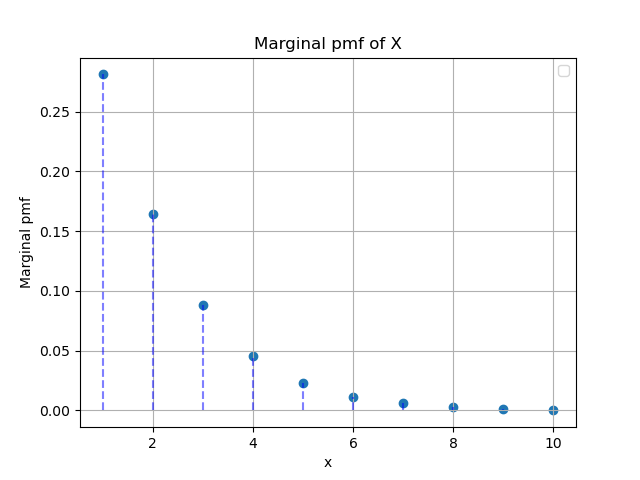
\includegraphics[width=\columnwidth]{/home/yogitha/47.2023/figs/pmfx.png}
\caption{Marginal pmf}
\label{fig:i_pmf}
\end{figure}
\end{enumerate}
Steps of simulation:
\begin{enumerate}
\item Define function p as $P\brak{x,y}=\frac{3}{2^{x+y+3}}$ in C and run a loop to sum the function p for all values of y except $x\neq y$, for each value of x.
\item Store values of marginal pmf for each value of x in a dat file 
\item Using plt.scatter function of python, plot the graph of Marginal pmf of X vs X.
The same can be used to plot marginal pmf of Y
\end{enumerate}

\item Let $X$ be a random variable with the probability density function $f(x)$ such that
\begin{align}
f(x) &= 
	\begin{cases}
		\frac{1}{2\sqrt{3}}, & -\sqrt{3} \leq x \leq \sqrt{3} \\
		0, & \text{otherwise}
	\end{cases}
\end{align}
Then the variance of $X$ is?
\hfill(GATE XH-C1 2023)
\\
\iffalse
\let\negmedspace\undefined
\let\negthickspace\undefined
\documentclass[journal,12pt,twocolumn]{IEEEtran}
\usepackage{cite}
\usepackage{amsmath,amssymb,amsfonts,amsthm}
\usepackage{algorithmic}
\usepackage{graphicx}
\usepackage{textcomp}
\usepackage{xcolor}
\usepackage{txfonts}
\usepackage{listings}
\usepackage{enumitem}
\usepackage{mathtools}
\usepackage{gensymb}
\usepackage[breaklinks=true]{hyperref}
\usepackage{tkz-euclide} % loads  TikZ and tkz-base
\usepackage{listings}
\usepackage{gvv}
\usepackage{float}  % To use the [H] placement specifier

%
%\usepackage{setspace}
%\usepackage{gensymb}
%\doublespacing
%\singlespacing

%\usepackage{graphicx}
%\usepackage{amssymb}
%\usepackage{relsize}
%\usepackage[cmex10]{amsmath}
%\usepackage{amsthm}
%\interdisplaylinepenalty=2500
%\savesymbol{iint}
%\usepackage{txfonts}
%\restoresymbol{TXF}{iint}
%\usepackage{wasysym}
%\usepackage{amsthm}
%\usepackage{iithtlc}
%\usepackage{mathrsfs}
%\usepackage{txfonts}
%\usepackage{stfloats}
%\usepackage{bm}
%\usepackage{cite}
%\usepackage{cases}
%\usepackage{subfig}
%\usepackage{xtab}
%\usepackage{longtable}
%\usepackage{multirow}
%\usepackage{algorithm}
%\usepackage{algpseudocode}
%\usepackage{enumitem}
%\usepackage{mathtools}
%\usepackage{tikz}
%\usepackage{circuitikz}
%\usepackage{verbatim}
%\usepackage{tfrupee}
%\usepackage{stmaryrd}
%\usetkzobj{all}
%    \usepackage{color}                                            %%
%    \usepackage{array}                                            %%
%    \usepackage{longtable}                                        %%
%    \usepackage{calc}                                             %%
%    \usepackage{multirow}                                         %%
%    \usepackage{hhline}                                           %%
%    \usepackage{ifthen}                                           %%
  %optionally (for landscape tables embedded in another document): %%
%    \usepackage{lscape}     
%\usepackage{multicol}
%\usepackage{chngcntr}
%\usepackage{enumerate}

%\usepackage{wasysym}
%\documentclass[conference]{IEEEtran}
%\IEEEoverridecommandlockouts
% The preceding line is only needed to identify funding in the first footnote. If that is unneeded, please comment it out.

\newtheorem{theorem}{Theorem}[section]
\newtheorem{problem}{Problem}
\newtheorem{proposition}{Proposition}[section]
\newtheorem{lemma}{Lemma}[section]
\newtheorem{corollary}[theorem]{Corollary}
\newtheorem{example}{Example}[section]
\newtheorem{definition}[problem]{Definition}
%\newtheorem{thm}{Theorem}[section] 
%\newtheorem{defn}[thm]{Definition}
%\newtheorem{algorithm}{Algorithm}[section]
%\newtheorem{cor}{Corollary}
\newcommand{\BEQA}{\begin{eqnarray}}
\newcommand{\EEQA}{\end{eqnarray}}
%\newcommand{\define}{\stackrel{\triangle}{=}}
\theoremstyle{remark}
\newtheorem{rem}{Remark}

%\bibliographystyle{ieeetr}
\begin{document}
%

\bibliographystyle{IEEEtran}


\vspace{3cm}

\title{
%	\logo{
	47
%	}
}
\author{ EE22BTECH11059% <-this % stops a space
}	
%\title{
%	\logo{Matrix Analysis through Octave}{\begin{center}\includegraphics[scale=.24]{tlc}\end{center}}{}{HAMDSP}
%}


% paper title
% can use linebreaks \\ within to get better formatting as desired
%\title{Matrix Analysis through Octave}
%
%
% author names and IEEE memberships
% note positions of commas and nonbreaking spaces ( ~ ) LaTeX will not break
% a structure at a ~ so this keeps an author's name from being broken across
% two lines.
% use \thanks{} to gain access to the first footnote area
% a separate \thanks must be used for each paragraph as LaTeX2e's \thanks
% was not built to handle multiple paragraphs
%

%\author{<-this % stops a space
%\thanks{}}
%}
% note the % following the last \IEEEmembership and also \thanks - 
% these prevent an unwanted space from occurring between the last author name
% and the end of the author line. i.e., if you had this:
% 
% \author{....lastname \thanks{...} \thanks{...} }
%                     ^------------^------------^----Do not want these spaces!
%
% a space would be appended to the last name and could cause every name on that
% line to be shifted left slightly. This is one of those "LaTeX things". For
% instance, "\textbf{A} \textbf{B}" will typeset as "A B" not "AB". To get
% "AB" then you have to do: "\textbf{A}\textbf{B}"
% \thanks is no different in this regard, so shield the last } of each \thanks
% that ends a line with a % and do not let a space in before the next \thanks.
% Spaces after \IEEEmembership other than the last one are OK (and needed) as
% you are supposed to have spaces between the names. For what it is worth,
% this is a minor point as most people would not even notice if the said evil
% space somehow managed to creep in.



% The paper headers
%\markboth{Journal of \LaTeX\ Class Files,~Vol.~6, No.~1, January~2007}%
%{Shell \MakeLowercase{\textit{et al.}}: Bare Demo of IEEEtran.cls for Journals}
% The only time the second header will appear is for the odd numbered pages
% after the title page when using the twoside option.
% 
% *** Note that you probably will NOT want to include the author's ***
% *** name in the headers of peer review papers.                   ***
% You can use \ifCLASSOPTIONpeerreview for conditional compilation here if
% you desire.




% If you want to put a publisher's ID mark on the page you can do it like
% this:
%\IEEEpubid{0000--0000/00\$00.00~\copyright~2007 IEEE}
% Remember, if you use this you must call \IEEEpubidadjcol in the second
% column for its text to clear the IEEEpubid mark.



% make the title area
\maketitle

\newpage

%\tableofcontents

\bigskip

\renewcommand{\thefigure}{\theenumi}
\renewcommand{\thetable}{\theenumi}
%\renewcommand{\theequation}{\theenumi}

%\begin{abstract}
%%\boldmath
%In this letter, an algorithm for evaluating the exact analytical bit error rate  (BER)  for the piecewise linear (PL) combiner for  multiple relays is presented. Previous results were available only for upto three relays. The algorithm is unique in the sense that  the actual mathematical expressions, that are prohibitively large, need not be explicitly obtained. The diversity gain due to multiple relays is shown through plots of the analytical BER, well supported by simulations. 
%
%\end{abstract}
% IEEEtran.cls defaults to using nonbold math in the Abstract.
% This preserves the distinction between vectors and scalars. However,
% if the journal you are submitting to favors bold math in the abstract,
% then you can use LaTeX's standard command \boldmath at the very start
% of the abstract to achieve this. Many IEEE journals frown on math
% in the abstract anyway.

% Note that keywords are not normally used for peerreview papers.
%\begin{IEEEkeywords}
%Cooperative diversity, decode and forward, piecewise linear
%\end{IEEEkeywords}



% For peer review papers, you can put extra information on the cover
% page as needed:
% \ifCLASSOPTIONpeerreview
% \begin{center} \bfseries EDICS Category: 3-BBND \end{center}
% \fi
%
% For peerreview papers, this IEEEtran command inserts a page break and
% creates the second title. It will be ignored for other modes.
%\IEEEpeerreviewmaketitle

%\documentclass{article}
%\usepackage{amsmath}
%\section*{ASSIGNMENT 1}
Let \brak{X,Y} have joint probability mass function 
\begin{align}
p\brak{x,y}=  
	\begin{cases}
        \frac{c}{2^{x+y+2}} & if x=0,1,2,... \, y=0,1,2,...; x\neq y \\
        0 & otherwise
        \end{cases} 
\end{align} 
Then which of the following is true?\\
\hfill (GATE ST 2023) \\
\begin{enumerate}
\item $c = \frac{1}{2}$
\item $c = \frac{1}{4}$
\item $c > 1$
\item $X$ and $Y$ are independent
\end{enumerate}
\fi
\solution
For p\brak{x,y} to be joint probability mass function
\begin{align}
\sum\limits^{\infty}_{y=-\infty}\sum\limits^{\infty}_{x=-\infty}p(x,y)&=1 \, \vert x \neq y\\
\sum\limits^{\infty}_{y=0}\sum\limits^{\infty}_{x=0}\frac{c}{2^{x+y+2}}- \sum\limits_{x=y} \frac{c}{2^{x+y+2}}&=1\\
\sum\limits^{\infty}_{y=0}\frac{c}{2^{y+2}} \sum\limits^{\infty}_{x=0} 2^{-x}- \frac{c}{4}\sum\limits^{\infty}_{x=0}\frac{1}{4^x}&=1\\
\sum\limits^{\infty}_{y=0}\frac{2c}{2^{y+2}}- \frac{c}{3}&=1\\
\frac{2c}{4}\sum\limits^{\infty}_{y=0}2^{-y}-\frac{c}{3}&=1\\
c-\frac{c}{3}&=1\\
c&=\frac{3}{2}
\end{align}
\begin{enumerate}
\item Marginal probability mass function of X
\begin{align}
p_X\brak{x}&=\sum\limits^{\infty}_{y=0}p\brak{x,y} \vert x \neq y\\
&=\sum\limits^{\infty}_{y=0}\frac{3}{2^{x+y+3}}- p_{XY}\brak{x,x}\\
&=\frac{3}{2^{x+3}}\sum\limits^{\infty}_{y=0}2^{-y}-\frac{3}{2^{2x+3}}\\
&=\frac{3}{2^{x+2}}-\frac{3}{2^{2x+3}}
\end{align}
\item Marginal cdf of X
\begin{align}
F_X\brak{x}&=\sum\limits^{x}_{i=0} p_X\brak{X \leq x}\\
&=\sum\limits^{x}_{i=0}\brak{\frac{3}{2^{x+2}}-\frac{3}{2^{2x+3}}}\\
&=1+\frac{1}{2^{x+2}}-\frac{3}{2^{2x+3}}
\end{align}
\item Marginal probability mass function of Y
\begin{align}
p_Y\brak{y}&=\sum\limits^{\infty}_{x=0}p\brak{x,y} \vert x \neq y\\
&=\sum\limits^{\infty}_{x=0}\frac{3}{2^{x+y+3}}- p_{XY}\brak{y,y}\\
&=\frac{3}{2^{y+3}}\sum\limits^{\infty}_{x=0}2^{-x}-\frac{3}{2^{2y+3}}\\
&=\frac{3}{2^{y+2}}-\frac{3}{2^{2y+3}}\\
\end{align}
\item Marginal cdf of Y
\begin{align}
F_Y\brak{y}&=\sum\limits^{y}_{i=0} p_Y\brak{Y \leq y}\\
&=\sum\limits^{y}_{i=0}\brak{\frac{3}{2^{y+2}}-\frac{3}{2^{2y+3}}}\\
&=1+\frac{1}{2^{y+2}}-\frac{3}{2^{2y+3}}
\end{align}
\item For X and Y to be independent,
\begin{align}
p\brak{x,y}&=p_X\brak{x} p_Y\brak{y}\\
p_X\brak{x} p_Y\brak{y}&=\brak{\frac{3}{2^{x+2}}-\frac{3}{2^{2x+3}}}\brak{\frac{3}{2^{y+2}}-\frac{3}{2^{2y+3}}}\\
p\brak{x,y} &\neq p_X\brak{x} p_Y\brak{y}
\end{align}
\end{enumerate}
Option \brak{4} is incorrect.\\
$\therefore$ Only option \brak{3} is correct. \\
Simulations:
\begin{enumerate}
\item Marginal pmf of X
\begin{figure}[H]
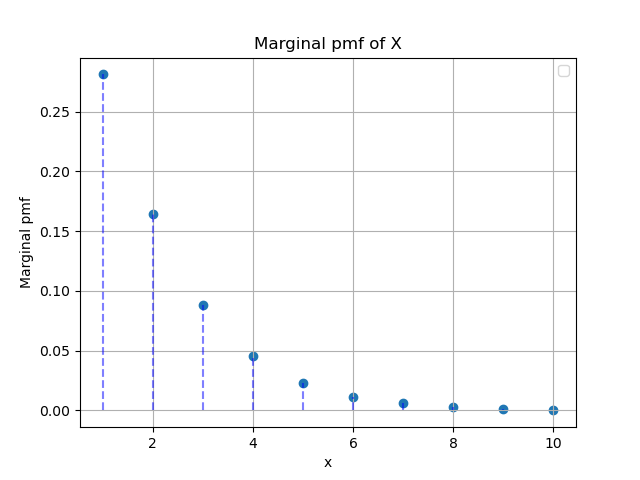
\includegraphics[width=\columnwidth]{/home/yogitha/47.2023/figs/pmfx.png}
\caption{Marginal pmf}
\label{fig:i_pmf}
\end{figure}
\end{enumerate}
Steps of simulation:
\begin{enumerate}
\item Define function p as $P\brak{x,y}=\frac{3}{2^{x+y+3}}$ in C and run a loop to sum the function p for all values of y except $x\neq y$, for each value of x.
\item Store values of marginal pmf for each value of x in a dat file 
\item Using plt.scatter function of python, plot the graph of Marginal pmf of X vs X.
The same can be used to plot marginal pmf of Y
\end{enumerate}

\item Two defective bulbs are present in a set of five bulbs. To remove the two
defective bulbs, the bulbs are chosen randomly one by one and tested. If $X$
denotes the minimum number of bulbs that must be tested to find out the two
defective bulbs, then $\pr{X=3}$ (rounded off to two decimal places)
equals\\
\hfill(GATE ST 2023)\\
\iffalse
\let\negmedspace\undefined
\let\negthickspace\undefined
\documentclass[journal,12pt,twocolumn]{IEEEtran}
\usepackage{cite}
\usepackage{amsmath,amssymb,amsfonts,amsthm}
\usepackage{algorithmic}
\usepackage{graphicx}
\usepackage{textcomp}
\usepackage{xcolor}
\usepackage{txfonts}
\usepackage{listings}
\usepackage{enumitem}
\usepackage{mathtools}
\usepackage{gensymb}
\usepackage[breaklinks=true]{hyperref}
\usepackage{tkz-euclide} % loads  TikZ and tkz-base
\usepackage{listings}
\usepackage{gvv}
\usepackage{float}  % To use the [H] placement specifier

%
%\usepackage{setspace}
%\usepackage{gensymb}
%\doublespacing
%\singlespacing

%\usepackage{graphicx}
%\usepackage{amssymb}
%\usepackage{relsize}
%\usepackage[cmex10]{amsmath}
%\usepackage{amsthm}
%\interdisplaylinepenalty=2500
%\savesymbol{iint}
%\usepackage{txfonts}
%\restoresymbol{TXF}{iint}
%\usepackage{wasysym}
%\usepackage{amsthm}
%\usepackage{iithtlc}
%\usepackage{mathrsfs}
%\usepackage{txfonts}
%\usepackage{stfloats}
%\usepackage{bm}
%\usepackage{cite}
%\usepackage{cases}
%\usepackage{subfig}
%\usepackage{xtab}
%\usepackage{longtable}
%\usepackage{multirow}
%\usepackage{algorithm}
%\usepackage{algpseudocode}
%\usepackage{enumitem}
%\usepackage{mathtools}
%\usepackage{tikz}
%\usepackage{circuitikz}
%\usepackage{verbatim}
%\usepackage{tfrupee}
%\usepackage{stmaryrd}
%\usetkzobj{all}
%    \usepackage{color}                                            %%
%    \usepackage{array}                                            %%
%    \usepackage{longtable}                                        %%
%    \usepackage{calc}                                             %%
%    \usepackage{multirow}                                         %%
%    \usepackage{hhline}                                           %%
%    \usepackage{ifthen}                                           %%
  %optionally (for landscape tables embedded in another document): %%
%    \usepackage{lscape}     
%\usepackage{multicol}
%\usepackage{chngcntr}
%\usepackage{enumerate}

%\usepackage{wasysym}
%\documentclass[conference]{IEEEtran}
%\IEEEoverridecommandlockouts
% The preceding line is only needed to identify funding in the first footnote. If that is unneeded, please comment it out.

\newtheorem{theorem}{Theorem}[section]
\newtheorem{problem}{Problem}
\newtheorem{proposition}{Proposition}[section]
\newtheorem{lemma}{Lemma}[section]
\newtheorem{corollary}[theorem]{Corollary}
\newtheorem{example}{Example}[section]
\newtheorem{definition}[problem]{Definition}
%\newtheorem{thm}{Theorem}[section] 
%\newtheorem{defn}[thm]{Definition}
%\newtheorem{algorithm}{Algorithm}[section]
%\newtheorem{cor}{Corollary}
\newcommand{\BEQA}{\begin{eqnarray}}
\newcommand{\EEQA}{\end{eqnarray}}
%\newcommand{\define}{\stackrel{\triangle}{=}}
\theoremstyle{remark}
\newtheorem{rem}{Remark}

%\bibliographystyle{ieeetr}
\begin{document}
%

\bibliographystyle{IEEEtran}


\vspace{3cm}

\title{
%	\logo{
	47
%	}
}
\author{ EE22BTECH11059% <-this % stops a space
}	
%\title{
%	\logo{Matrix Analysis through Octave}{\begin{center}\includegraphics[scale=.24]{tlc}\end{center}}{}{HAMDSP}
%}


% paper title
% can use linebreaks \\ within to get better formatting as desired
%\title{Matrix Analysis through Octave}
%
%
% author names and IEEE memberships
% note positions of commas and nonbreaking spaces ( ~ ) LaTeX will not break
% a structure at a ~ so this keeps an author's name from being broken across
% two lines.
% use \thanks{} to gain access to the first footnote area
% a separate \thanks must be used for each paragraph as LaTeX2e's \thanks
% was not built to handle multiple paragraphs
%

%\author{<-this % stops a space
%\thanks{}}
%}
% note the % following the last \IEEEmembership and also \thanks - 
% these prevent an unwanted space from occurring between the last author name
% and the end of the author line. i.e., if you had this:
% 
% \author{....lastname \thanks{...} \thanks{...} }
%                     ^------------^------------^----Do not want these spaces!
%
% a space would be appended to the last name and could cause every name on that
% line to be shifted left slightly. This is one of those "LaTeX things". For
% instance, "\textbf{A} \textbf{B}" will typeset as "A B" not "AB". To get
% "AB" then you have to do: "\textbf{A}\textbf{B}"
% \thanks is no different in this regard, so shield the last } of each \thanks
% that ends a line with a % and do not let a space in before the next \thanks.
% Spaces after \IEEEmembership other than the last one are OK (and needed) as
% you are supposed to have spaces between the names. For what it is worth,
% this is a minor point as most people would not even notice if the said evil
% space somehow managed to creep in.



% The paper headers
%\markboth{Journal of \LaTeX\ Class Files,~Vol.~6, No.~1, January~2007}%
%{Shell \MakeLowercase{\textit{et al.}}: Bare Demo of IEEEtran.cls for Journals}
% The only time the second header will appear is for the odd numbered pages
% after the title page when using the twoside option.
% 
% *** Note that you probably will NOT want to include the author's ***
% *** name in the headers of peer review papers.                   ***
% You can use \ifCLASSOPTIONpeerreview for conditional compilation here if
% you desire.




% If you want to put a publisher's ID mark on the page you can do it like
% this:
%\IEEEpubid{0000--0000/00\$00.00~\copyright~2007 IEEE}
% Remember, if you use this you must call \IEEEpubidadjcol in the second
% column for its text to clear the IEEEpubid mark.



% make the title area
\maketitle

\newpage

%\tableofcontents

\bigskip

\renewcommand{\thefigure}{\theenumi}
\renewcommand{\thetable}{\theenumi}
%\renewcommand{\theequation}{\theenumi}

%\begin{abstract}
%%\boldmath
%In this letter, an algorithm for evaluating the exact analytical bit error rate  (BER)  for the piecewise linear (PL) combiner for  multiple relays is presented. Previous results were available only for upto three relays. The algorithm is unique in the sense that  the actual mathematical expressions, that are prohibitively large, need not be explicitly obtained. The diversity gain due to multiple relays is shown through plots of the analytical BER, well supported by simulations. 
%
%\end{abstract}
% IEEEtran.cls defaults to using nonbold math in the Abstract.
% This preserves the distinction between vectors and scalars. However,
% if the journal you are submitting to favors bold math in the abstract,
% then you can use LaTeX's standard command \boldmath at the very start
% of the abstract to achieve this. Many IEEE journals frown on math
% in the abstract anyway.

% Note that keywords are not normally used for peerreview papers.
%\begin{IEEEkeywords}
%Cooperative diversity, decode and forward, piecewise linear
%\end{IEEEkeywords}



% For peer review papers, you can put extra information on the cover
% page as needed:
% \ifCLASSOPTIONpeerreview
% \begin{center} \bfseries EDICS Category: 3-BBND \end{center}
% \fi
%
% For peerreview papers, this IEEEtran command inserts a page break and
% creates the second title. It will be ignored for other modes.
%\IEEEpeerreviewmaketitle

%\documentclass{article}
%\usepackage{amsmath}
%\section*{ASSIGNMENT 1}
Let \brak{X,Y} have joint probability mass function 
\begin{align}
p\brak{x,y}=  
	\begin{cases}
        \frac{c}{2^{x+y+2}} & if x=0,1,2,... \, y=0,1,2,...; x\neq y \\
        0 & otherwise
        \end{cases} 
\end{align} 
Then which of the following is true?\\
\hfill (GATE ST 2023) \\
\begin{enumerate}
\item $c = \frac{1}{2}$
\item $c = \frac{1}{4}$
\item $c > 1$
\item $X$ and $Y$ are independent
\end{enumerate}
\fi
\solution
For p\brak{x,y} to be joint probability mass function
\begin{align}
\sum\limits^{\infty}_{y=-\infty}\sum\limits^{\infty}_{x=-\infty}p(x,y)&=1 \, \vert x \neq y\\
\sum\limits^{\infty}_{y=0}\sum\limits^{\infty}_{x=0}\frac{c}{2^{x+y+2}}- \sum\limits_{x=y} \frac{c}{2^{x+y+2}}&=1\\
\sum\limits^{\infty}_{y=0}\frac{c}{2^{y+2}} \sum\limits^{\infty}_{x=0} 2^{-x}- \frac{c}{4}\sum\limits^{\infty}_{x=0}\frac{1}{4^x}&=1\\
\sum\limits^{\infty}_{y=0}\frac{2c}{2^{y+2}}- \frac{c}{3}&=1\\
\frac{2c}{4}\sum\limits^{\infty}_{y=0}2^{-y}-\frac{c}{3}&=1\\
c-\frac{c}{3}&=1\\
c&=\frac{3}{2}
\end{align}
\begin{enumerate}
\item Marginal probability mass function of X
\begin{align}
p_X\brak{x}&=\sum\limits^{\infty}_{y=0}p\brak{x,y} \vert x \neq y\\
&=\sum\limits^{\infty}_{y=0}\frac{3}{2^{x+y+3}}- p_{XY}\brak{x,x}\\
&=\frac{3}{2^{x+3}}\sum\limits^{\infty}_{y=0}2^{-y}-\frac{3}{2^{2x+3}}\\
&=\frac{3}{2^{x+2}}-\frac{3}{2^{2x+3}}
\end{align}
\item Marginal cdf of X
\begin{align}
F_X\brak{x}&=\sum\limits^{x}_{i=0} p_X\brak{X \leq x}\\
&=\sum\limits^{x}_{i=0}\brak{\frac{3}{2^{x+2}}-\frac{3}{2^{2x+3}}}\\
&=1+\frac{1}{2^{x+2}}-\frac{3}{2^{2x+3}}
\end{align}
\item Marginal probability mass function of Y
\begin{align}
p_Y\brak{y}&=\sum\limits^{\infty}_{x=0}p\brak{x,y} \vert x \neq y\\
&=\sum\limits^{\infty}_{x=0}\frac{3}{2^{x+y+3}}- p_{XY}\brak{y,y}\\
&=\frac{3}{2^{y+3}}\sum\limits^{\infty}_{x=0}2^{-x}-\frac{3}{2^{2y+3}}\\
&=\frac{3}{2^{y+2}}-\frac{3}{2^{2y+3}}\\
\end{align}
\item Marginal cdf of Y
\begin{align}
F_Y\brak{y}&=\sum\limits^{y}_{i=0} p_Y\brak{Y \leq y}\\
&=\sum\limits^{y}_{i=0}\brak{\frac{3}{2^{y+2}}-\frac{3}{2^{2y+3}}}\\
&=1+\frac{1}{2^{y+2}}-\frac{3}{2^{2y+3}}
\end{align}
\item For X and Y to be independent,
\begin{align}
p\brak{x,y}&=p_X\brak{x} p_Y\brak{y}\\
p_X\brak{x} p_Y\brak{y}&=\brak{\frac{3}{2^{x+2}}-\frac{3}{2^{2x+3}}}\brak{\frac{3}{2^{y+2}}-\frac{3}{2^{2y+3}}}\\
p\brak{x,y} &\neq p_X\brak{x} p_Y\brak{y}
\end{align}
\end{enumerate}
Option \brak{4} is incorrect.\\
$\therefore$ Only option \brak{3} is correct. \\
Simulations:
\begin{enumerate}
\item Marginal pmf of X
\begin{figure}[H]
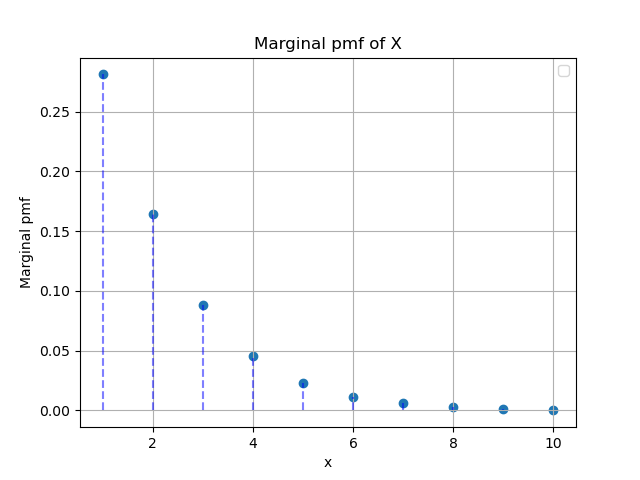
\includegraphics[width=\columnwidth]{/home/yogitha/47.2023/figs/pmfx.png}
\caption{Marginal pmf}
\label{fig:i_pmf}
\end{figure}
\end{enumerate}
Steps of simulation:
\begin{enumerate}
\item Define function p as $P\brak{x,y}=\frac{3}{2^{x+y+3}}$ in C and run a loop to sum the function p for all values of y except $x\neq y$, for each value of x.
\item Store values of marginal pmf for each value of x in a dat file 
\item Using plt.scatter function of python, plot the graph of Marginal pmf of X vs X.
The same can be used to plot marginal pmf of Y
\end{enumerate}

\item Let $X$ be a random variable with cumulative distribution function
\begin{align}
F_X(x) &= 
	\begin{cases}
		0 & \text{if $x < -1$}\\
		\frac{1}{4}\brak{x+1} & \text{if $-1 \leq x < 0$}\\
		\frac{1}{4}\brak{x+3} & \text{if $0 \leq x < 1$}\\
		1 & \text{if $ x \geq 1$}\\
	\end{cases}
\end{align}
Which one of the following statements is true?
\begin{enumerate}[label=(\Alph*)]
    \item\begin{align} \lim_{n \to \infty} \pr{-\frac{1}{2} + \frac{1}{n} < X < -\frac{1}{n}} = \frac{5}{8}\end{align}
    \item \begin{align}\lim_{n \to \infty} \pr{-\frac{1}{2} - \frac{1}{n} < X < \frac{1}{n}} = \frac{5}{8}\end{align}
    \item \begin{align}\lim_{n \to \infty} \pr{X = \frac{1}{n}} = \frac{1}{2}\end{align}
    \item \begin{align}\pr{X = 0} = \frac{1}{3}\end{align}
\end{enumerate}

\hfill(GATE ST 2023)\\
\iffalse
\let\negmedspace\undefined
\let\negthickspace\undefined
\documentclass[journal,12pt,twocolumn]{IEEEtran}
\usepackage{cite}
\usepackage{amsmath,amssymb,amsfonts,amsthm}
\usepackage{algorithmic}
\usepackage{graphicx}
\usepackage{textcomp}
\usepackage{xcolor}
\usepackage{txfonts}
\usepackage{listings}
\usepackage{enumitem}
\usepackage{mathtools}
\usepackage{gensymb}
\usepackage[breaklinks=true]{hyperref}
\usepackage{tkz-euclide} % loads  TikZ and tkz-base
\usepackage{listings}
\usepackage{gvv}
\usepackage{float}  % To use the [H] placement specifier

%
%\usepackage{setspace}
%\usepackage{gensymb}
%\doublespacing
%\singlespacing

%\usepackage{graphicx}
%\usepackage{amssymb}
%\usepackage{relsize}
%\usepackage[cmex10]{amsmath}
%\usepackage{amsthm}
%\interdisplaylinepenalty=2500
%\savesymbol{iint}
%\usepackage{txfonts}
%\restoresymbol{TXF}{iint}
%\usepackage{wasysym}
%\usepackage{amsthm}
%\usepackage{iithtlc}
%\usepackage{mathrsfs}
%\usepackage{txfonts}
%\usepackage{stfloats}
%\usepackage{bm}
%\usepackage{cite}
%\usepackage{cases}
%\usepackage{subfig}
%\usepackage{xtab}
%\usepackage{longtable}
%\usepackage{multirow}
%\usepackage{algorithm}
%\usepackage{algpseudocode}
%\usepackage{enumitem}
%\usepackage{mathtools}
%\usepackage{tikz}
%\usepackage{circuitikz}
%\usepackage{verbatim}
%\usepackage{tfrupee}
%\usepackage{stmaryrd}
%\usetkzobj{all}
%    \usepackage{color}                                            %%
%    \usepackage{array}                                            %%
%    \usepackage{longtable}                                        %%
%    \usepackage{calc}                                             %%
%    \usepackage{multirow}                                         %%
%    \usepackage{hhline}                                           %%
%    \usepackage{ifthen}                                           %%
  %optionally (for landscape tables embedded in another document): %%
%    \usepackage{lscape}     
%\usepackage{multicol}
%\usepackage{chngcntr}
%\usepackage{enumerate}

%\usepackage{wasysym}
%\documentclass[conference]{IEEEtran}
%\IEEEoverridecommandlockouts
% The preceding line is only needed to identify funding in the first footnote. If that is unneeded, please comment it out.

\newtheorem{theorem}{Theorem}[section]
\newtheorem{problem}{Problem}
\newtheorem{proposition}{Proposition}[section]
\newtheorem{lemma}{Lemma}[section]
\newtheorem{corollary}[theorem]{Corollary}
\newtheorem{example}{Example}[section]
\newtheorem{definition}[problem]{Definition}
%\newtheorem{thm}{Theorem}[section] 
%\newtheorem{defn}[thm]{Definition}
%\newtheorem{algorithm}{Algorithm}[section]
%\newtheorem{cor}{Corollary}
\newcommand{\BEQA}{\begin{eqnarray}}
\newcommand{\EEQA}{\end{eqnarray}}
%\newcommand{\define}{\stackrel{\triangle}{=}}
\theoremstyle{remark}
\newtheorem{rem}{Remark}

%\bibliographystyle{ieeetr}
\begin{document}
%

\bibliographystyle{IEEEtran}


\vspace{3cm}

\title{
%	\logo{
	47
%	}
}
\author{ EE22BTECH11059% <-this % stops a space
}	
%\title{
%	\logo{Matrix Analysis through Octave}{\begin{center}\includegraphics[scale=.24]{tlc}\end{center}}{}{HAMDSP}
%}


% paper title
% can use linebreaks \\ within to get better formatting as desired
%\title{Matrix Analysis through Octave}
%
%
% author names and IEEE memberships
% note positions of commas and nonbreaking spaces ( ~ ) LaTeX will not break
% a structure at a ~ so this keeps an author's name from being broken across
% two lines.
% use \thanks{} to gain access to the first footnote area
% a separate \thanks must be used for each paragraph as LaTeX2e's \thanks
% was not built to handle multiple paragraphs
%

%\author{<-this % stops a space
%\thanks{}}
%}
% note the % following the last \IEEEmembership and also \thanks - 
% these prevent an unwanted space from occurring between the last author name
% and the end of the author line. i.e., if you had this:
% 
% \author{....lastname \thanks{...} \thanks{...} }
%                     ^------------^------------^----Do not want these spaces!
%
% a space would be appended to the last name and could cause every name on that
% line to be shifted left slightly. This is one of those "LaTeX things". For
% instance, "\textbf{A} \textbf{B}" will typeset as "A B" not "AB". To get
% "AB" then you have to do: "\textbf{A}\textbf{B}"
% \thanks is no different in this regard, so shield the last } of each \thanks
% that ends a line with a % and do not let a space in before the next \thanks.
% Spaces after \IEEEmembership other than the last one are OK (and needed) as
% you are supposed to have spaces between the names. For what it is worth,
% this is a minor point as most people would not even notice if the said evil
% space somehow managed to creep in.



% The paper headers
%\markboth{Journal of \LaTeX\ Class Files,~Vol.~6, No.~1, January~2007}%
%{Shell \MakeLowercase{\textit{et al.}}: Bare Demo of IEEEtran.cls for Journals}
% The only time the second header will appear is for the odd numbered pages
% after the title page when using the twoside option.
% 
% *** Note that you probably will NOT want to include the author's ***
% *** name in the headers of peer review papers.                   ***
% You can use \ifCLASSOPTIONpeerreview for conditional compilation here if
% you desire.




% If you want to put a publisher's ID mark on the page you can do it like
% this:
%\IEEEpubid{0000--0000/00\$00.00~\copyright~2007 IEEE}
% Remember, if you use this you must call \IEEEpubidadjcol in the second
% column for its text to clear the IEEEpubid mark.



% make the title area
\maketitle

\newpage

%\tableofcontents

\bigskip

\renewcommand{\thefigure}{\theenumi}
\renewcommand{\thetable}{\theenumi}
%\renewcommand{\theequation}{\theenumi}

%\begin{abstract}
%%\boldmath
%In this letter, an algorithm for evaluating the exact analytical bit error rate  (BER)  for the piecewise linear (PL) combiner for  multiple relays is presented. Previous results were available only for upto three relays. The algorithm is unique in the sense that  the actual mathematical expressions, that are prohibitively large, need not be explicitly obtained. The diversity gain due to multiple relays is shown through plots of the analytical BER, well supported by simulations. 
%
%\end{abstract}
% IEEEtran.cls defaults to using nonbold math in the Abstract.
% This preserves the distinction between vectors and scalars. However,
% if the journal you are submitting to favors bold math in the abstract,
% then you can use LaTeX's standard command \boldmath at the very start
% of the abstract to achieve this. Many IEEE journals frown on math
% in the abstract anyway.

% Note that keywords are not normally used for peerreview papers.
%\begin{IEEEkeywords}
%Cooperative diversity, decode and forward, piecewise linear
%\end{IEEEkeywords}



% For peer review papers, you can put extra information on the cover
% page as needed:
% \ifCLASSOPTIONpeerreview
% \begin{center} \bfseries EDICS Category: 3-BBND \end{center}
% \fi
%
% For peerreview papers, this IEEEtran command inserts a page break and
% creates the second title. It will be ignored for other modes.
%\IEEEpeerreviewmaketitle

%\documentclass{article}
%\usepackage{amsmath}
%\section*{ASSIGNMENT 1}
Let \brak{X,Y} have joint probability mass function 
\begin{align}
p\brak{x,y}=  
	\begin{cases}
        \frac{c}{2^{x+y+2}} & if x=0,1,2,... \, y=0,1,2,...; x\neq y \\
        0 & otherwise
        \end{cases} 
\end{align} 
Then which of the following is true?\\
\hfill (GATE ST 2023) \\
\begin{enumerate}
\item $c = \frac{1}{2}$
\item $c = \frac{1}{4}$
\item $c > 1$
\item $X$ and $Y$ are independent
\end{enumerate}
\fi
\solution
For p\brak{x,y} to be joint probability mass function
\begin{align}
\sum\limits^{\infty}_{y=-\infty}\sum\limits^{\infty}_{x=-\infty}p(x,y)&=1 \, \vert x \neq y\\
\sum\limits^{\infty}_{y=0}\sum\limits^{\infty}_{x=0}\frac{c}{2^{x+y+2}}- \sum\limits_{x=y} \frac{c}{2^{x+y+2}}&=1\\
\sum\limits^{\infty}_{y=0}\frac{c}{2^{y+2}} \sum\limits^{\infty}_{x=0} 2^{-x}- \frac{c}{4}\sum\limits^{\infty}_{x=0}\frac{1}{4^x}&=1\\
\sum\limits^{\infty}_{y=0}\frac{2c}{2^{y+2}}- \frac{c}{3}&=1\\
\frac{2c}{4}\sum\limits^{\infty}_{y=0}2^{-y}-\frac{c}{3}&=1\\
c-\frac{c}{3}&=1\\
c&=\frac{3}{2}
\end{align}
\begin{enumerate}
\item Marginal probability mass function of X
\begin{align}
p_X\brak{x}&=\sum\limits^{\infty}_{y=0}p\brak{x,y} \vert x \neq y\\
&=\sum\limits^{\infty}_{y=0}\frac{3}{2^{x+y+3}}- p_{XY}\brak{x,x}\\
&=\frac{3}{2^{x+3}}\sum\limits^{\infty}_{y=0}2^{-y}-\frac{3}{2^{2x+3}}\\
&=\frac{3}{2^{x+2}}-\frac{3}{2^{2x+3}}
\end{align}
\item Marginal cdf of X
\begin{align}
F_X\brak{x}&=\sum\limits^{x}_{i=0} p_X\brak{X \leq x}\\
&=\sum\limits^{x}_{i=0}\brak{\frac{3}{2^{x+2}}-\frac{3}{2^{2x+3}}}\\
&=1+\frac{1}{2^{x+2}}-\frac{3}{2^{2x+3}}
\end{align}
\item Marginal probability mass function of Y
\begin{align}
p_Y\brak{y}&=\sum\limits^{\infty}_{x=0}p\brak{x,y} \vert x \neq y\\
&=\sum\limits^{\infty}_{x=0}\frac{3}{2^{x+y+3}}- p_{XY}\brak{y,y}\\
&=\frac{3}{2^{y+3}}\sum\limits^{\infty}_{x=0}2^{-x}-\frac{3}{2^{2y+3}}\\
&=\frac{3}{2^{y+2}}-\frac{3}{2^{2y+3}}\\
\end{align}
\item Marginal cdf of Y
\begin{align}
F_Y\brak{y}&=\sum\limits^{y}_{i=0} p_Y\brak{Y \leq y}\\
&=\sum\limits^{y}_{i=0}\brak{\frac{3}{2^{y+2}}-\frac{3}{2^{2y+3}}}\\
&=1+\frac{1}{2^{y+2}}-\frac{3}{2^{2y+3}}
\end{align}
\item For X and Y to be independent,
\begin{align}
p\brak{x,y}&=p_X\brak{x} p_Y\brak{y}\\
p_X\brak{x} p_Y\brak{y}&=\brak{\frac{3}{2^{x+2}}-\frac{3}{2^{2x+3}}}\brak{\frac{3}{2^{y+2}}-\frac{3}{2^{2y+3}}}\\
p\brak{x,y} &\neq p_X\brak{x} p_Y\brak{y}
\end{align}
\end{enumerate}
Option \brak{4} is incorrect.\\
$\therefore$ Only option \brak{3} is correct. \\
Simulations:
\begin{enumerate}
\item Marginal pmf of X
\begin{figure}[H]
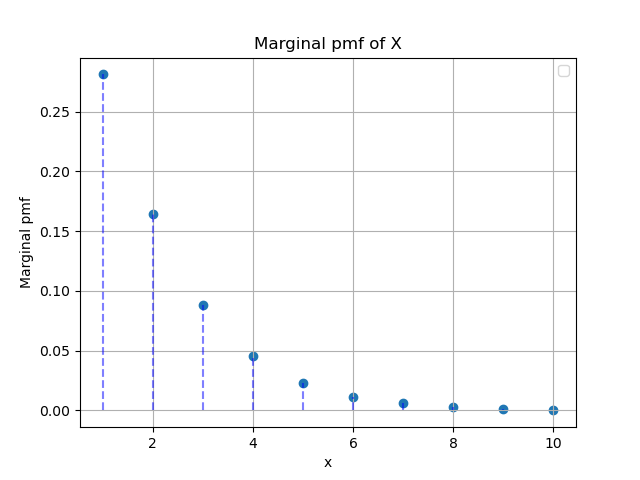
\includegraphics[width=\columnwidth]{/home/yogitha/47.2023/figs/pmfx.png}
\caption{Marginal pmf}
\label{fig:i_pmf}
\end{figure}
\end{enumerate}
Steps of simulation:
\begin{enumerate}
\item Define function p as $P\brak{x,y}=\frac{3}{2^{x+y+3}}$ in C and run a loop to sum the function p for all values of y except $x\neq y$, for each value of x.
\item Store values of marginal pmf for each value of x in a dat file 
\item Using plt.scatter function of python, plot the graph of Marginal pmf of X vs X.
The same can be used to plot marginal pmf of Y
\end{enumerate}

\item Three unbiased coins were tossed. Provided that at least two outcomes are tails,the probability of having all three outcomes as tails is\\
\hfill(GATE PI 2023)\\
\iffalse
\let\negmedspace\undefined
\let\negthickspace\undefined
\documentclass[journal,12pt,twocolumn]{IEEEtran}
\usepackage{cite}
\usepackage{amsmath,amssymb,amsfonts,amsthm}
\usepackage{algorithmic}
\usepackage{graphicx}
\usepackage{textcomp}
\usepackage{xcolor}
\usepackage{txfonts}
\usepackage{listings}
\usepackage{enumitem}
\usepackage{mathtools}
\usepackage{gensymb}
\usepackage[breaklinks=true]{hyperref}
\usepackage{tkz-euclide} % loads  TikZ and tkz-base
\usepackage{listings}
\usepackage{gvv}
\usepackage{float}  % To use the [H] placement specifier

%
%\usepackage{setspace}
%\usepackage{gensymb}
%\doublespacing
%\singlespacing

%\usepackage{graphicx}
%\usepackage{amssymb}
%\usepackage{relsize}
%\usepackage[cmex10]{amsmath}
%\usepackage{amsthm}
%\interdisplaylinepenalty=2500
%\savesymbol{iint}
%\usepackage{txfonts}
%\restoresymbol{TXF}{iint}
%\usepackage{wasysym}
%\usepackage{amsthm}
%\usepackage{iithtlc}
%\usepackage{mathrsfs}
%\usepackage{txfonts}
%\usepackage{stfloats}
%\usepackage{bm}
%\usepackage{cite}
%\usepackage{cases}
%\usepackage{subfig}
%\usepackage{xtab}
%\usepackage{longtable}
%\usepackage{multirow}
%\usepackage{algorithm}
%\usepackage{algpseudocode}
%\usepackage{enumitem}
%\usepackage{mathtools}
%\usepackage{tikz}
%\usepackage{circuitikz}
%\usepackage{verbatim}
%\usepackage{tfrupee}
%\usepackage{stmaryrd}
%\usetkzobj{all}
%    \usepackage{color}                                            %%
%    \usepackage{array}                                            %%
%    \usepackage{longtable}                                        %%
%    \usepackage{calc}                                             %%
%    \usepackage{multirow}                                         %%
%    \usepackage{hhline}                                           %%
%    \usepackage{ifthen}                                           %%
  %optionally (for landscape tables embedded in another document): %%
%    \usepackage{lscape}     
%\usepackage{multicol}
%\usepackage{chngcntr}
%\usepackage{enumerate}

%\usepackage{wasysym}
%\documentclass[conference]{IEEEtran}
%\IEEEoverridecommandlockouts
% The preceding line is only needed to identify funding in the first footnote. If that is unneeded, please comment it out.

\newtheorem{theorem}{Theorem}[section]
\newtheorem{problem}{Problem}
\newtheorem{proposition}{Proposition}[section]
\newtheorem{lemma}{Lemma}[section]
\newtheorem{corollary}[theorem]{Corollary}
\newtheorem{example}{Example}[section]
\newtheorem{definition}[problem]{Definition}
%\newtheorem{thm}{Theorem}[section] 
%\newtheorem{defn}[thm]{Definition}
%\newtheorem{algorithm}{Algorithm}[section]
%\newtheorem{cor}{Corollary}
\newcommand{\BEQA}{\begin{eqnarray}}
\newcommand{\EEQA}{\end{eqnarray}}
%\newcommand{\define}{\stackrel{\triangle}{=}}
\theoremstyle{remark}
\newtheorem{rem}{Remark}

%\bibliographystyle{ieeetr}
\begin{document}
%

\bibliographystyle{IEEEtran}


\vspace{3cm}

\title{
%	\logo{
	47
%	}
}
\author{ EE22BTECH11059% <-this % stops a space
}	
%\title{
%	\logo{Matrix Analysis through Octave}{\begin{center}\includegraphics[scale=.24]{tlc}\end{center}}{}{HAMDSP}
%}


% paper title
% can use linebreaks \\ within to get better formatting as desired
%\title{Matrix Analysis through Octave}
%
%
% author names and IEEE memberships
% note positions of commas and nonbreaking spaces ( ~ ) LaTeX will not break
% a structure at a ~ so this keeps an author's name from being broken across
% two lines.
% use \thanks{} to gain access to the first footnote area
% a separate \thanks must be used for each paragraph as LaTeX2e's \thanks
% was not built to handle multiple paragraphs
%

%\author{<-this % stops a space
%\thanks{}}
%}
% note the % following the last \IEEEmembership and also \thanks - 
% these prevent an unwanted space from occurring between the last author name
% and the end of the author line. i.e., if you had this:
% 
% \author{....lastname \thanks{...} \thanks{...} }
%                     ^------------^------------^----Do not want these spaces!
%
% a space would be appended to the last name and could cause every name on that
% line to be shifted left slightly. This is one of those "LaTeX things". For
% instance, "\textbf{A} \textbf{B}" will typeset as "A B" not "AB". To get
% "AB" then you have to do: "\textbf{A}\textbf{B}"
% \thanks is no different in this regard, so shield the last } of each \thanks
% that ends a line with a % and do not let a space in before the next \thanks.
% Spaces after \IEEEmembership other than the last one are OK (and needed) as
% you are supposed to have spaces between the names. For what it is worth,
% this is a minor point as most people would not even notice if the said evil
% space somehow managed to creep in.



% The paper headers
%\markboth{Journal of \LaTeX\ Class Files,~Vol.~6, No.~1, January~2007}%
%{Shell \MakeLowercase{\textit{et al.}}: Bare Demo of IEEEtran.cls for Journals}
% The only time the second header will appear is for the odd numbered pages
% after the title page when using the twoside option.
% 
% *** Note that you probably will NOT want to include the author's ***
% *** name in the headers of peer review papers.                   ***
% You can use \ifCLASSOPTIONpeerreview for conditional compilation here if
% you desire.




% If you want to put a publisher's ID mark on the page you can do it like
% this:
%\IEEEpubid{0000--0000/00\$00.00~\copyright~2007 IEEE}
% Remember, if you use this you must call \IEEEpubidadjcol in the second
% column for its text to clear the IEEEpubid mark.



% make the title area
\maketitle

\newpage

%\tableofcontents

\bigskip

\renewcommand{\thefigure}{\theenumi}
\renewcommand{\thetable}{\theenumi}
%\renewcommand{\theequation}{\theenumi}

%\begin{abstract}
%%\boldmath
%In this letter, an algorithm for evaluating the exact analytical bit error rate  (BER)  for the piecewise linear (PL) combiner for  multiple relays is presented. Previous results were available only for upto three relays. The algorithm is unique in the sense that  the actual mathematical expressions, that are prohibitively large, need not be explicitly obtained. The diversity gain due to multiple relays is shown through plots of the analytical BER, well supported by simulations. 
%
%\end{abstract}
% IEEEtran.cls defaults to using nonbold math in the Abstract.
% This preserves the distinction between vectors and scalars. However,
% if the journal you are submitting to favors bold math in the abstract,
% then you can use LaTeX's standard command \boldmath at the very start
% of the abstract to achieve this. Many IEEE journals frown on math
% in the abstract anyway.

% Note that keywords are not normally used for peerreview papers.
%\begin{IEEEkeywords}
%Cooperative diversity, decode and forward, piecewise linear
%\end{IEEEkeywords}



% For peer review papers, you can put extra information on the cover
% page as needed:
% \ifCLASSOPTIONpeerreview
% \begin{center} \bfseries EDICS Category: 3-BBND \end{center}
% \fi
%
% For peerreview papers, this IEEEtran command inserts a page break and
% creates the second title. It will be ignored for other modes.
%\IEEEpeerreviewmaketitle

%\documentclass{article}
%\usepackage{amsmath}
%\section*{ASSIGNMENT 1}
Let \brak{X,Y} have joint probability mass function 
\begin{align}
p\brak{x,y}=  
	\begin{cases}
        \frac{c}{2^{x+y+2}} & if x=0,1,2,... \, y=0,1,2,...; x\neq y \\
        0 & otherwise
        \end{cases} 
\end{align} 
Then which of the following is true?\\
\hfill (GATE ST 2023) \\
\begin{enumerate}
\item $c = \frac{1}{2}$
\item $c = \frac{1}{4}$
\item $c > 1$
\item $X$ and $Y$ are independent
\end{enumerate}
\fi
\solution
For p\brak{x,y} to be joint probability mass function
\begin{align}
\sum\limits^{\infty}_{y=-\infty}\sum\limits^{\infty}_{x=-\infty}p(x,y)&=1 \, \vert x \neq y\\
\sum\limits^{\infty}_{y=0}\sum\limits^{\infty}_{x=0}\frac{c}{2^{x+y+2}}- \sum\limits_{x=y} \frac{c}{2^{x+y+2}}&=1\\
\sum\limits^{\infty}_{y=0}\frac{c}{2^{y+2}} \sum\limits^{\infty}_{x=0} 2^{-x}- \frac{c}{4}\sum\limits^{\infty}_{x=0}\frac{1}{4^x}&=1\\
\sum\limits^{\infty}_{y=0}\frac{2c}{2^{y+2}}- \frac{c}{3}&=1\\
\frac{2c}{4}\sum\limits^{\infty}_{y=0}2^{-y}-\frac{c}{3}&=1\\
c-\frac{c}{3}&=1\\
c&=\frac{3}{2}
\end{align}
\begin{enumerate}
\item Marginal probability mass function of X
\begin{align}
p_X\brak{x}&=\sum\limits^{\infty}_{y=0}p\brak{x,y} \vert x \neq y\\
&=\sum\limits^{\infty}_{y=0}\frac{3}{2^{x+y+3}}- p_{XY}\brak{x,x}\\
&=\frac{3}{2^{x+3}}\sum\limits^{\infty}_{y=0}2^{-y}-\frac{3}{2^{2x+3}}\\
&=\frac{3}{2^{x+2}}-\frac{3}{2^{2x+3}}
\end{align}
\item Marginal cdf of X
\begin{align}
F_X\brak{x}&=\sum\limits^{x}_{i=0} p_X\brak{X \leq x}\\
&=\sum\limits^{x}_{i=0}\brak{\frac{3}{2^{x+2}}-\frac{3}{2^{2x+3}}}\\
&=1+\frac{1}{2^{x+2}}-\frac{3}{2^{2x+3}}
\end{align}
\item Marginal probability mass function of Y
\begin{align}
p_Y\brak{y}&=\sum\limits^{\infty}_{x=0}p\brak{x,y} \vert x \neq y\\
&=\sum\limits^{\infty}_{x=0}\frac{3}{2^{x+y+3}}- p_{XY}\brak{y,y}\\
&=\frac{3}{2^{y+3}}\sum\limits^{\infty}_{x=0}2^{-x}-\frac{3}{2^{2y+3}}\\
&=\frac{3}{2^{y+2}}-\frac{3}{2^{2y+3}}\\
\end{align}
\item Marginal cdf of Y
\begin{align}
F_Y\brak{y}&=\sum\limits^{y}_{i=0} p_Y\brak{Y \leq y}\\
&=\sum\limits^{y}_{i=0}\brak{\frac{3}{2^{y+2}}-\frac{3}{2^{2y+3}}}\\
&=1+\frac{1}{2^{y+2}}-\frac{3}{2^{2y+3}}
\end{align}
\item For X and Y to be independent,
\begin{align}
p\brak{x,y}&=p_X\brak{x} p_Y\brak{y}\\
p_X\brak{x} p_Y\brak{y}&=\brak{\frac{3}{2^{x+2}}-\frac{3}{2^{2x+3}}}\brak{\frac{3}{2^{y+2}}-\frac{3}{2^{2y+3}}}\\
p\brak{x,y} &\neq p_X\brak{x} p_Y\brak{y}
\end{align}
\end{enumerate}
Option \brak{4} is incorrect.\\
$\therefore$ Only option \brak{3} is correct. \\
Simulations:
\begin{enumerate}
\item Marginal pmf of X
\begin{figure}[H]
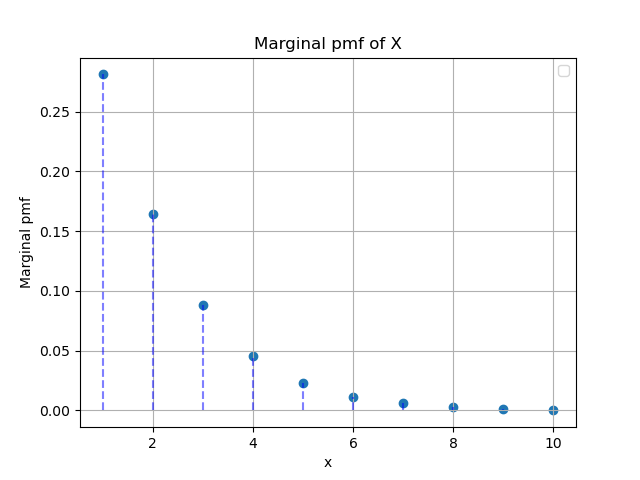
\includegraphics[width=\columnwidth]{/home/yogitha/47.2023/figs/pmfx.png}
\caption{Marginal pmf}
\label{fig:i_pmf}
\end{figure}
\end{enumerate}
Steps of simulation:
\begin{enumerate}
\item Define function p as $P\brak{x,y}=\frac{3}{2^{x+y+3}}$ in C and run a loop to sum the function p for all values of y except $x\neq y$, for each value of x.
\item Store values of marginal pmf for each value of x in a dat file 
\item Using plt.scatter function of python, plot the graph of Marginal pmf of X vs X.
The same can be used to plot marginal pmf of Y
\end{enumerate}

\item Let $X$ be a random variable with probability density function
\begin{align}
p_{X}\brak{x}=\begin{cases}
		e^{-x} & if x\ge 0\\ 
		0 & otherwise
	\end{cases}
\end{align}
For $a<b$, if $U\brak{a,b}$ denotes the uniform distribution over the interval $\brak{a,b}$,
then which of the following statements is/are true?
\begin{enumerate}[label=(\Alph*)]
\item $e^{-X}$ follows $U\brak{-1,0}$ distribution
\item $1-e^{-X}$follows $U\brak{0,2}$ distribution
\item $2e^{-X}-1$follows $U\brak{-1,1}$ distribution
\item The probability mass function of $Y=\sbrak{X}$ is
$\pr{Y=k}=e^{-k}\brak{1-e^{-1}}$ for k= 0, 1, 2, …,
where $\sbrak{X}$denotes the largest integer not exceeding $x$
\end{enumerate}
\hfill(GATE ST 2023)\\
\solution
\iffalse
\let\negmedspace\undefined
\let\negthickspace\undefined
\documentclass[journal,12pt,twocolumn]{IEEEtran}
\usepackage{cite}
\usepackage{amsmath,amssymb,amsfonts,amsthm}
\usepackage{algorithmic}
\usepackage{graphicx}
\usepackage{textcomp}
\usepackage{xcolor}
\usepackage{txfonts}
\usepackage{listings}
\usepackage{enumitem}
\usepackage{mathtools}
\usepackage{gensymb}
\usepackage[breaklinks=true]{hyperref}
\usepackage{tkz-euclide} % loads  TikZ and tkz-base
\usepackage{listings}
\usepackage{gvv}
\usepackage{float}  % To use the [H] placement specifier

%
%\usepackage{setspace}
%\usepackage{gensymb}
%\doublespacing
%\singlespacing

%\usepackage{graphicx}
%\usepackage{amssymb}
%\usepackage{relsize}
%\usepackage[cmex10]{amsmath}
%\usepackage{amsthm}
%\interdisplaylinepenalty=2500
%\savesymbol{iint}
%\usepackage{txfonts}
%\restoresymbol{TXF}{iint}
%\usepackage{wasysym}
%\usepackage{amsthm}
%\usepackage{iithtlc}
%\usepackage{mathrsfs}
%\usepackage{txfonts}
%\usepackage{stfloats}
%\usepackage{bm}
%\usepackage{cite}
%\usepackage{cases}
%\usepackage{subfig}
%\usepackage{xtab}
%\usepackage{longtable}
%\usepackage{multirow}
%\usepackage{algorithm}
%\usepackage{algpseudocode}
%\usepackage{enumitem}
%\usepackage{mathtools}
%\usepackage{tikz}
%\usepackage{circuitikz}
%\usepackage{verbatim}
%\usepackage{tfrupee}
%\usepackage{stmaryrd}
%\usetkzobj{all}
%    \usepackage{color}                                            %%
%    \usepackage{array}                                            %%
%    \usepackage{longtable}                                        %%
%    \usepackage{calc}                                             %%
%    \usepackage{multirow}                                         %%
%    \usepackage{hhline}                                           %%
%    \usepackage{ifthen}                                           %%
  %optionally (for landscape tables embedded in another document): %%
%    \usepackage{lscape}     
%\usepackage{multicol}
%\usepackage{chngcntr}
%\usepackage{enumerate}

%\usepackage{wasysym}
%\documentclass[conference]{IEEEtran}
%\IEEEoverridecommandlockouts
% The preceding line is only needed to identify funding in the first footnote. If that is unneeded, please comment it out.

\newtheorem{theorem}{Theorem}[section]
\newtheorem{problem}{Problem}
\newtheorem{proposition}{Proposition}[section]
\newtheorem{lemma}{Lemma}[section]
\newtheorem{corollary}[theorem]{Corollary}
\newtheorem{example}{Example}[section]
\newtheorem{definition}[problem]{Definition}
%\newtheorem{thm}{Theorem}[section] 
%\newtheorem{defn}[thm]{Definition}
%\newtheorem{algorithm}{Algorithm}[section]
%\newtheorem{cor}{Corollary}
\newcommand{\BEQA}{\begin{eqnarray}}
\newcommand{\EEQA}{\end{eqnarray}}
%\newcommand{\define}{\stackrel{\triangle}{=}}
\theoremstyle{remark}
\newtheorem{rem}{Remark}

%\bibliographystyle{ieeetr}
\begin{document}
%

\bibliographystyle{IEEEtran}


\vspace{3cm}

\title{
%	\logo{
	47
%	}
}
\author{ EE22BTECH11059% <-this % stops a space
}	
%\title{
%	\logo{Matrix Analysis through Octave}{\begin{center}\includegraphics[scale=.24]{tlc}\end{center}}{}{HAMDSP}
%}


% paper title
% can use linebreaks \\ within to get better formatting as desired
%\title{Matrix Analysis through Octave}
%
%
% author names and IEEE memberships
% note positions of commas and nonbreaking spaces ( ~ ) LaTeX will not break
% a structure at a ~ so this keeps an author's name from being broken across
% two lines.
% use \thanks{} to gain access to the first footnote area
% a separate \thanks must be used for each paragraph as LaTeX2e's \thanks
% was not built to handle multiple paragraphs
%

%\author{<-this % stops a space
%\thanks{}}
%}
% note the % following the last \IEEEmembership and also \thanks - 
% these prevent an unwanted space from occurring between the last author name
% and the end of the author line. i.e., if you had this:
% 
% \author{....lastname \thanks{...} \thanks{...} }
%                     ^------------^------------^----Do not want these spaces!
%
% a space would be appended to the last name and could cause every name on that
% line to be shifted left slightly. This is one of those "LaTeX things". For
% instance, "\textbf{A} \textbf{B}" will typeset as "A B" not "AB". To get
% "AB" then you have to do: "\textbf{A}\textbf{B}"
% \thanks is no different in this regard, so shield the last } of each \thanks
% that ends a line with a % and do not let a space in before the next \thanks.
% Spaces after \IEEEmembership other than the last one are OK (and needed) as
% you are supposed to have spaces between the names. For what it is worth,
% this is a minor point as most people would not even notice if the said evil
% space somehow managed to creep in.



% The paper headers
%\markboth{Journal of \LaTeX\ Class Files,~Vol.~6, No.~1, January~2007}%
%{Shell \MakeLowercase{\textit{et al.}}: Bare Demo of IEEEtran.cls for Journals}
% The only time the second header will appear is for the odd numbered pages
% after the title page when using the twoside option.
% 
% *** Note that you probably will NOT want to include the author's ***
% *** name in the headers of peer review papers.                   ***
% You can use \ifCLASSOPTIONpeerreview for conditional compilation here if
% you desire.




% If you want to put a publisher's ID mark on the page you can do it like
% this:
%\IEEEpubid{0000--0000/00\$00.00~\copyright~2007 IEEE}
% Remember, if you use this you must call \IEEEpubidadjcol in the second
% column for its text to clear the IEEEpubid mark.



% make the title area
\maketitle

\newpage

%\tableofcontents

\bigskip

\renewcommand{\thefigure}{\theenumi}
\renewcommand{\thetable}{\theenumi}
%\renewcommand{\theequation}{\theenumi}

%\begin{abstract}
%%\boldmath
%In this letter, an algorithm for evaluating the exact analytical bit error rate  (BER)  for the piecewise linear (PL) combiner for  multiple relays is presented. Previous results were available only for upto three relays. The algorithm is unique in the sense that  the actual mathematical expressions, that are prohibitively large, need not be explicitly obtained. The diversity gain due to multiple relays is shown through plots of the analytical BER, well supported by simulations. 
%
%\end{abstract}
% IEEEtran.cls defaults to using nonbold math in the Abstract.
% This preserves the distinction between vectors and scalars. However,
% if the journal you are submitting to favors bold math in the abstract,
% then you can use LaTeX's standard command \boldmath at the very start
% of the abstract to achieve this. Many IEEE journals frown on math
% in the abstract anyway.

% Note that keywords are not normally used for peerreview papers.
%\begin{IEEEkeywords}
%Cooperative diversity, decode and forward, piecewise linear
%\end{IEEEkeywords}



% For peer review papers, you can put extra information on the cover
% page as needed:
% \ifCLASSOPTIONpeerreview
% \begin{center} \bfseries EDICS Category: 3-BBND \end{center}
% \fi
%
% For peerreview papers, this IEEEtran command inserts a page break and
% creates the second title. It will be ignored for other modes.
%\IEEEpeerreviewmaketitle

%\documentclass{article}
%\usepackage{amsmath}
%\section*{ASSIGNMENT 1}
Let \brak{X,Y} have joint probability mass function 
\begin{align}
p\brak{x,y}=  
	\begin{cases}
        \frac{c}{2^{x+y+2}} & if x=0,1,2,... \, y=0,1,2,...; x\neq y \\
        0 & otherwise
        \end{cases} 
\end{align} 
Then which of the following is true?\\
\hfill (GATE ST 2023) \\
\begin{enumerate}
\item $c = \frac{1}{2}$
\item $c = \frac{1}{4}$
\item $c > 1$
\item $X$ and $Y$ are independent
\end{enumerate}
\fi
\solution
For p\brak{x,y} to be joint probability mass function
\begin{align}
\sum\limits^{\infty}_{y=-\infty}\sum\limits^{\infty}_{x=-\infty}p(x,y)&=1 \, \vert x \neq y\\
\sum\limits^{\infty}_{y=0}\sum\limits^{\infty}_{x=0}\frac{c}{2^{x+y+2}}- \sum\limits_{x=y} \frac{c}{2^{x+y+2}}&=1\\
\sum\limits^{\infty}_{y=0}\frac{c}{2^{y+2}} \sum\limits^{\infty}_{x=0} 2^{-x}- \frac{c}{4}\sum\limits^{\infty}_{x=0}\frac{1}{4^x}&=1\\
\sum\limits^{\infty}_{y=0}\frac{2c}{2^{y+2}}- \frac{c}{3}&=1\\
\frac{2c}{4}\sum\limits^{\infty}_{y=0}2^{-y}-\frac{c}{3}&=1\\
c-\frac{c}{3}&=1\\
c&=\frac{3}{2}
\end{align}
\begin{enumerate}
\item Marginal probability mass function of X
\begin{align}
p_X\brak{x}&=\sum\limits^{\infty}_{y=0}p\brak{x,y} \vert x \neq y\\
&=\sum\limits^{\infty}_{y=0}\frac{3}{2^{x+y+3}}- p_{XY}\brak{x,x}\\
&=\frac{3}{2^{x+3}}\sum\limits^{\infty}_{y=0}2^{-y}-\frac{3}{2^{2x+3}}\\
&=\frac{3}{2^{x+2}}-\frac{3}{2^{2x+3}}
\end{align}
\item Marginal cdf of X
\begin{align}
F_X\brak{x}&=\sum\limits^{x}_{i=0} p_X\brak{X \leq x}\\
&=\sum\limits^{x}_{i=0}\brak{\frac{3}{2^{x+2}}-\frac{3}{2^{2x+3}}}\\
&=1+\frac{1}{2^{x+2}}-\frac{3}{2^{2x+3}}
\end{align}
\item Marginal probability mass function of Y
\begin{align}
p_Y\brak{y}&=\sum\limits^{\infty}_{x=0}p\brak{x,y} \vert x \neq y\\
&=\sum\limits^{\infty}_{x=0}\frac{3}{2^{x+y+3}}- p_{XY}\brak{y,y}\\
&=\frac{3}{2^{y+3}}\sum\limits^{\infty}_{x=0}2^{-x}-\frac{3}{2^{2y+3}}\\
&=\frac{3}{2^{y+2}}-\frac{3}{2^{2y+3}}\\
\end{align}
\item Marginal cdf of Y
\begin{align}
F_Y\brak{y}&=\sum\limits^{y}_{i=0} p_Y\brak{Y \leq y}\\
&=\sum\limits^{y}_{i=0}\brak{\frac{3}{2^{y+2}}-\frac{3}{2^{2y+3}}}\\
&=1+\frac{1}{2^{y+2}}-\frac{3}{2^{2y+3}}
\end{align}
\item For X and Y to be independent,
\begin{align}
p\brak{x,y}&=p_X\brak{x} p_Y\brak{y}\\
p_X\brak{x} p_Y\brak{y}&=\brak{\frac{3}{2^{x+2}}-\frac{3}{2^{2x+3}}}\brak{\frac{3}{2^{y+2}}-\frac{3}{2^{2y+3}}}\\
p\brak{x,y} &\neq p_X\brak{x} p_Y\brak{y}
\end{align}
\end{enumerate}
Option \brak{4} is incorrect.\\
$\therefore$ Only option \brak{3} is correct. \\
Simulations:
\begin{enumerate}
\item Marginal pmf of X
\begin{figure}[H]
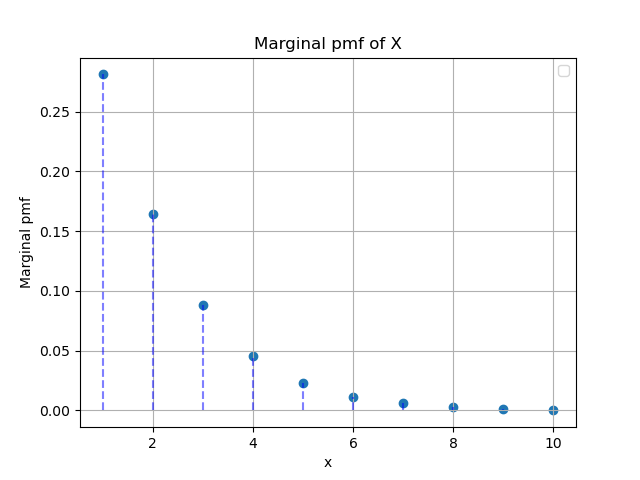
\includegraphics[width=\columnwidth]{/home/yogitha/47.2023/figs/pmfx.png}
\caption{Marginal pmf}
\label{fig:i_pmf}
\end{figure}
\end{enumerate}
Steps of simulation:
\begin{enumerate}
\item Define function p as $P\brak{x,y}=\frac{3}{2^{x+y+3}}$ in C and run a loop to sum the function p for all values of y except $x\neq y$, for each value of x.
\item Store values of marginal pmf for each value of x in a dat file 
\item Using plt.scatter function of python, plot the graph of Marginal pmf of X vs X.
The same can be used to plot marginal pmf of Y
\end{enumerate}

\item Question: Let $X$ be a positive valued continuous random variable with finite mean $\mu$.
If $Y=[X]$, the largest integer less than or equal to $X$, then which of the
following statements is/are true?
\begin{enumerate}[label=(\Alph*)]
\item $\pr{Y \leq \mu} \leq \pr{X \leq \mu}$ for all $\mu \geq 0$
\item $\pr{Y \geq \mu} \leq \pr{X \geq \mu}$ for all $\mu \geq 0$
\item E(X) $<$ E(Y)
\item E(X) $>$ E(Y)
\end{enumerate}
\hfill(GATE ST 2023)\\
\iffalse
\let\negmedspace\undefined
\let\negthickspace\undefined
\documentclass[journal,12pt,twocolumn]{IEEEtran}
\usepackage{cite}
\usepackage{amsmath,amssymb,amsfonts,amsthm}
\usepackage{algorithmic}
\usepackage{graphicx}
\usepackage{textcomp}
\usepackage{xcolor}
\usepackage{txfonts}
\usepackage{listings}
\usepackage{enumitem}
\usepackage{mathtools}
\usepackage{gensymb}
\usepackage[breaklinks=true]{hyperref}
\usepackage{tkz-euclide} % loads  TikZ and tkz-base
\usepackage{listings}
\usepackage{gvv}
\usepackage{float}  % To use the [H] placement specifier

%
%\usepackage{setspace}
%\usepackage{gensymb}
%\doublespacing
%\singlespacing

%\usepackage{graphicx}
%\usepackage{amssymb}
%\usepackage{relsize}
%\usepackage[cmex10]{amsmath}
%\usepackage{amsthm}
%\interdisplaylinepenalty=2500
%\savesymbol{iint}
%\usepackage{txfonts}
%\restoresymbol{TXF}{iint}
%\usepackage{wasysym}
%\usepackage{amsthm}
%\usepackage{iithtlc}
%\usepackage{mathrsfs}
%\usepackage{txfonts}
%\usepackage{stfloats}
%\usepackage{bm}
%\usepackage{cite}
%\usepackage{cases}
%\usepackage{subfig}
%\usepackage{xtab}
%\usepackage{longtable}
%\usepackage{multirow}
%\usepackage{algorithm}
%\usepackage{algpseudocode}
%\usepackage{enumitem}
%\usepackage{mathtools}
%\usepackage{tikz}
%\usepackage{circuitikz}
%\usepackage{verbatim}
%\usepackage{tfrupee}
%\usepackage{stmaryrd}
%\usetkzobj{all}
%    \usepackage{color}                                            %%
%    \usepackage{array}                                            %%
%    \usepackage{longtable}                                        %%
%    \usepackage{calc}                                             %%
%    \usepackage{multirow}                                         %%
%    \usepackage{hhline}                                           %%
%    \usepackage{ifthen}                                           %%
  %optionally (for landscape tables embedded in another document): %%
%    \usepackage{lscape}     
%\usepackage{multicol}
%\usepackage{chngcntr}
%\usepackage{enumerate}

%\usepackage{wasysym}
%\documentclass[conference]{IEEEtran}
%\IEEEoverridecommandlockouts
% The preceding line is only needed to identify funding in the first footnote. If that is unneeded, please comment it out.

\newtheorem{theorem}{Theorem}[section]
\newtheorem{problem}{Problem}
\newtheorem{proposition}{Proposition}[section]
\newtheorem{lemma}{Lemma}[section]
\newtheorem{corollary}[theorem]{Corollary}
\newtheorem{example}{Example}[section]
\newtheorem{definition}[problem]{Definition}
%\newtheorem{thm}{Theorem}[section] 
%\newtheorem{defn}[thm]{Definition}
%\newtheorem{algorithm}{Algorithm}[section]
%\newtheorem{cor}{Corollary}
\newcommand{\BEQA}{\begin{eqnarray}}
\newcommand{\EEQA}{\end{eqnarray}}
%\newcommand{\define}{\stackrel{\triangle}{=}}
\theoremstyle{remark}
\newtheorem{rem}{Remark}

%\bibliographystyle{ieeetr}
\begin{document}
%

\bibliographystyle{IEEEtran}


\vspace{3cm}

\title{
%	\logo{
	47
%	}
}
\author{ EE22BTECH11059% <-this % stops a space
}	
%\title{
%	\logo{Matrix Analysis through Octave}{\begin{center}\includegraphics[scale=.24]{tlc}\end{center}}{}{HAMDSP}
%}


% paper title
% can use linebreaks \\ within to get better formatting as desired
%\title{Matrix Analysis through Octave}
%
%
% author names and IEEE memberships
% note positions of commas and nonbreaking spaces ( ~ ) LaTeX will not break
% a structure at a ~ so this keeps an author's name from being broken across
% two lines.
% use \thanks{} to gain access to the first footnote area
% a separate \thanks must be used for each paragraph as LaTeX2e's \thanks
% was not built to handle multiple paragraphs
%

%\author{<-this % stops a space
%\thanks{}}
%}
% note the % following the last \IEEEmembership and also \thanks - 
% these prevent an unwanted space from occurring between the last author name
% and the end of the author line. i.e., if you had this:
% 
% \author{....lastname \thanks{...} \thanks{...} }
%                     ^------------^------------^----Do not want these spaces!
%
% a space would be appended to the last name and could cause every name on that
% line to be shifted left slightly. This is one of those "LaTeX things". For
% instance, "\textbf{A} \textbf{B}" will typeset as "A B" not "AB". To get
% "AB" then you have to do: "\textbf{A}\textbf{B}"
% \thanks is no different in this regard, so shield the last } of each \thanks
% that ends a line with a % and do not let a space in before the next \thanks.
% Spaces after \IEEEmembership other than the last one are OK (and needed) as
% you are supposed to have spaces between the names. For what it is worth,
% this is a minor point as most people would not even notice if the said evil
% space somehow managed to creep in.



% The paper headers
%\markboth{Journal of \LaTeX\ Class Files,~Vol.~6, No.~1, January~2007}%
%{Shell \MakeLowercase{\textit{et al.}}: Bare Demo of IEEEtran.cls for Journals}
% The only time the second header will appear is for the odd numbered pages
% after the title page when using the twoside option.
% 
% *** Note that you probably will NOT want to include the author's ***
% *** name in the headers of peer review papers.                   ***
% You can use \ifCLASSOPTIONpeerreview for conditional compilation here if
% you desire.




% If you want to put a publisher's ID mark on the page you can do it like
% this:
%\IEEEpubid{0000--0000/00\$00.00~\copyright~2007 IEEE}
% Remember, if you use this you must call \IEEEpubidadjcol in the second
% column for its text to clear the IEEEpubid mark.



% make the title area
\maketitle

\newpage

%\tableofcontents

\bigskip

\renewcommand{\thefigure}{\theenumi}
\renewcommand{\thetable}{\theenumi}
%\renewcommand{\theequation}{\theenumi}

%\begin{abstract}
%%\boldmath
%In this letter, an algorithm for evaluating the exact analytical bit error rate  (BER)  for the piecewise linear (PL) combiner for  multiple relays is presented. Previous results were available only for upto three relays. The algorithm is unique in the sense that  the actual mathematical expressions, that are prohibitively large, need not be explicitly obtained. The diversity gain due to multiple relays is shown through plots of the analytical BER, well supported by simulations. 
%
%\end{abstract}
% IEEEtran.cls defaults to using nonbold math in the Abstract.
% This preserves the distinction between vectors and scalars. However,
% if the journal you are submitting to favors bold math in the abstract,
% then you can use LaTeX's standard command \boldmath at the very start
% of the abstract to achieve this. Many IEEE journals frown on math
% in the abstract anyway.

% Note that keywords are not normally used for peerreview papers.
%\begin{IEEEkeywords}
%Cooperative diversity, decode and forward, piecewise linear
%\end{IEEEkeywords}



% For peer review papers, you can put extra information on the cover
% page as needed:
% \ifCLASSOPTIONpeerreview
% \begin{center} \bfseries EDICS Category: 3-BBND \end{center}
% \fi
%
% For peerreview papers, this IEEEtran command inserts a page break and
% creates the second title. It will be ignored for other modes.
%\IEEEpeerreviewmaketitle

%\documentclass{article}
%\usepackage{amsmath}
%\section*{ASSIGNMENT 1}
Let \brak{X,Y} have joint probability mass function 
\begin{align}
p\brak{x,y}=  
	\begin{cases}
        \frac{c}{2^{x+y+2}} & if x=0,1,2,... \, y=0,1,2,...; x\neq y \\
        0 & otherwise
        \end{cases} 
\end{align} 
Then which of the following is true?\\
\hfill (GATE ST 2023) \\
\begin{enumerate}
\item $c = \frac{1}{2}$
\item $c = \frac{1}{4}$
\item $c > 1$
\item $X$ and $Y$ are independent
\end{enumerate}
\fi
\solution
For p\brak{x,y} to be joint probability mass function
\begin{align}
\sum\limits^{\infty}_{y=-\infty}\sum\limits^{\infty}_{x=-\infty}p(x,y)&=1 \, \vert x \neq y\\
\sum\limits^{\infty}_{y=0}\sum\limits^{\infty}_{x=0}\frac{c}{2^{x+y+2}}- \sum\limits_{x=y} \frac{c}{2^{x+y+2}}&=1\\
\sum\limits^{\infty}_{y=0}\frac{c}{2^{y+2}} \sum\limits^{\infty}_{x=0} 2^{-x}- \frac{c}{4}\sum\limits^{\infty}_{x=0}\frac{1}{4^x}&=1\\
\sum\limits^{\infty}_{y=0}\frac{2c}{2^{y+2}}- \frac{c}{3}&=1\\
\frac{2c}{4}\sum\limits^{\infty}_{y=0}2^{-y}-\frac{c}{3}&=1\\
c-\frac{c}{3}&=1\\
c&=\frac{3}{2}
\end{align}
\begin{enumerate}
\item Marginal probability mass function of X
\begin{align}
p_X\brak{x}&=\sum\limits^{\infty}_{y=0}p\brak{x,y} \vert x \neq y\\
&=\sum\limits^{\infty}_{y=0}\frac{3}{2^{x+y+3}}- p_{XY}\brak{x,x}\\
&=\frac{3}{2^{x+3}}\sum\limits^{\infty}_{y=0}2^{-y}-\frac{3}{2^{2x+3}}\\
&=\frac{3}{2^{x+2}}-\frac{3}{2^{2x+3}}
\end{align}
\item Marginal cdf of X
\begin{align}
F_X\brak{x}&=\sum\limits^{x}_{i=0} p_X\brak{X \leq x}\\
&=\sum\limits^{x}_{i=0}\brak{\frac{3}{2^{x+2}}-\frac{3}{2^{2x+3}}}\\
&=1+\frac{1}{2^{x+2}}-\frac{3}{2^{2x+3}}
\end{align}
\item Marginal probability mass function of Y
\begin{align}
p_Y\brak{y}&=\sum\limits^{\infty}_{x=0}p\brak{x,y} \vert x \neq y\\
&=\sum\limits^{\infty}_{x=0}\frac{3}{2^{x+y+3}}- p_{XY}\brak{y,y}\\
&=\frac{3}{2^{y+3}}\sum\limits^{\infty}_{x=0}2^{-x}-\frac{3}{2^{2y+3}}\\
&=\frac{3}{2^{y+2}}-\frac{3}{2^{2y+3}}\\
\end{align}
\item Marginal cdf of Y
\begin{align}
F_Y\brak{y}&=\sum\limits^{y}_{i=0} p_Y\brak{Y \leq y}\\
&=\sum\limits^{y}_{i=0}\brak{\frac{3}{2^{y+2}}-\frac{3}{2^{2y+3}}}\\
&=1+\frac{1}{2^{y+2}}-\frac{3}{2^{2y+3}}
\end{align}
\item For X and Y to be independent,
\begin{align}
p\brak{x,y}&=p_X\brak{x} p_Y\brak{y}\\
p_X\brak{x} p_Y\brak{y}&=\brak{\frac{3}{2^{x+2}}-\frac{3}{2^{2x+3}}}\brak{\frac{3}{2^{y+2}}-\frac{3}{2^{2y+3}}}\\
p\brak{x,y} &\neq p_X\brak{x} p_Y\brak{y}
\end{align}
\end{enumerate}
Option \brak{4} is incorrect.\\
$\therefore$ Only option \brak{3} is correct. \\
Simulations:
\begin{enumerate}
\item Marginal pmf of X
\begin{figure}[H]
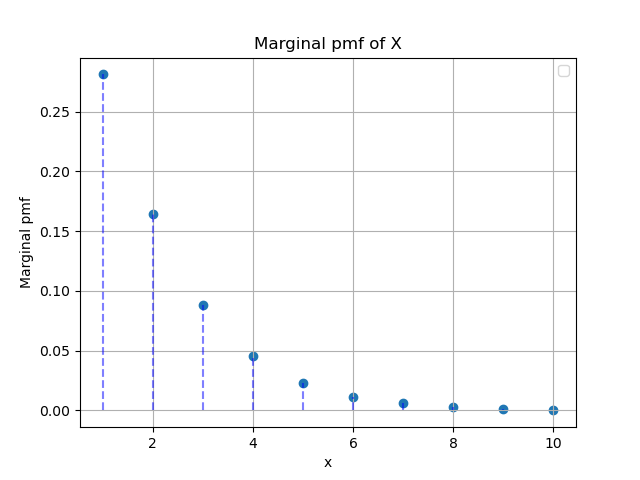
\includegraphics[width=\columnwidth]{/home/yogitha/47.2023/figs/pmfx.png}
\caption{Marginal pmf}
\label{fig:i_pmf}
\end{figure}
\end{enumerate}
Steps of simulation:
\begin{enumerate}
\item Define function p as $P\brak{x,y}=\frac{3}{2^{x+y+3}}$ in C and run a loop to sum the function p for all values of y except $x\neq y$, for each value of x.
\item Store values of marginal pmf for each value of x in a dat file 
\item Using plt.scatter function of python, plot the graph of Marginal pmf of X vs X.
The same can be used to plot marginal pmf of Y
\end{enumerate}

\item In a diploid angiosperm species, flower colour is regulated by the R gene.
RR and Rr genotypes produce red flowers, whereas the rr genotype produces
white flowers. If two individual plants are randomly selected from a large
segregating population of a genetic cross between RR and rr parents, the
probability of both the plants producing red flowers is\\
\hfill(GATE XL 2023)\\
\iffalse
\let\negmedspace\undefined
\let\negthickspace\undefined
\documentclass[journal,12pt,twocolumn]{IEEEtran}
\usepackage{cite}
\usepackage{amsmath,amssymb,amsfonts,amsthm}
\usepackage{algorithmic}
\usepackage{graphicx}
\usepackage{textcomp}
\usepackage{xcolor}
\usepackage{txfonts}
\usepackage{listings}
\usepackage{enumitem}
\usepackage{mathtools}
\usepackage{gensymb}
\usepackage[breaklinks=true]{hyperref}
\usepackage{tkz-euclide} % loads  TikZ and tkz-base
\usepackage{listings}
\usepackage{gvv}
\usepackage{float}  % To use the [H] placement specifier

%
%\usepackage{setspace}
%\usepackage{gensymb}
%\doublespacing
%\singlespacing

%\usepackage{graphicx}
%\usepackage{amssymb}
%\usepackage{relsize}
%\usepackage[cmex10]{amsmath}
%\usepackage{amsthm}
%\interdisplaylinepenalty=2500
%\savesymbol{iint}
%\usepackage{txfonts}
%\restoresymbol{TXF}{iint}
%\usepackage{wasysym}
%\usepackage{amsthm}
%\usepackage{iithtlc}
%\usepackage{mathrsfs}
%\usepackage{txfonts}
%\usepackage{stfloats}
%\usepackage{bm}
%\usepackage{cite}
%\usepackage{cases}
%\usepackage{subfig}
%\usepackage{xtab}
%\usepackage{longtable}
%\usepackage{multirow}
%\usepackage{algorithm}
%\usepackage{algpseudocode}
%\usepackage{enumitem}
%\usepackage{mathtools}
%\usepackage{tikz}
%\usepackage{circuitikz}
%\usepackage{verbatim}
%\usepackage{tfrupee}
%\usepackage{stmaryrd}
%\usetkzobj{all}
%    \usepackage{color}                                            %%
%    \usepackage{array}                                            %%
%    \usepackage{longtable}                                        %%
%    \usepackage{calc}                                             %%
%    \usepackage{multirow}                                         %%
%    \usepackage{hhline}                                           %%
%    \usepackage{ifthen}                                           %%
  %optionally (for landscape tables embedded in another document): %%
%    \usepackage{lscape}     
%\usepackage{multicol}
%\usepackage{chngcntr}
%\usepackage{enumerate}

%\usepackage{wasysym}
%\documentclass[conference]{IEEEtran}
%\IEEEoverridecommandlockouts
% The preceding line is only needed to identify funding in the first footnote. If that is unneeded, please comment it out.

\newtheorem{theorem}{Theorem}[section]
\newtheorem{problem}{Problem}
\newtheorem{proposition}{Proposition}[section]
\newtheorem{lemma}{Lemma}[section]
\newtheorem{corollary}[theorem]{Corollary}
\newtheorem{example}{Example}[section]
\newtheorem{definition}[problem]{Definition}
%\newtheorem{thm}{Theorem}[section] 
%\newtheorem{defn}[thm]{Definition}
%\newtheorem{algorithm}{Algorithm}[section]
%\newtheorem{cor}{Corollary}
\newcommand{\BEQA}{\begin{eqnarray}}
\newcommand{\EEQA}{\end{eqnarray}}
%\newcommand{\define}{\stackrel{\triangle}{=}}
\theoremstyle{remark}
\newtheorem{rem}{Remark}

%\bibliographystyle{ieeetr}
\begin{document}
%

\bibliographystyle{IEEEtran}


\vspace{3cm}

\title{
%	\logo{
	47
%	}
}
\author{ EE22BTECH11059% <-this % stops a space
}	
%\title{
%	\logo{Matrix Analysis through Octave}{\begin{center}\includegraphics[scale=.24]{tlc}\end{center}}{}{HAMDSP}
%}


% paper title
% can use linebreaks \\ within to get better formatting as desired
%\title{Matrix Analysis through Octave}
%
%
% author names and IEEE memberships
% note positions of commas and nonbreaking spaces ( ~ ) LaTeX will not break
% a structure at a ~ so this keeps an author's name from being broken across
% two lines.
% use \thanks{} to gain access to the first footnote area
% a separate \thanks must be used for each paragraph as LaTeX2e's \thanks
% was not built to handle multiple paragraphs
%

%\author{<-this % stops a space
%\thanks{}}
%}
% note the % following the last \IEEEmembership and also \thanks - 
% these prevent an unwanted space from occurring between the last author name
% and the end of the author line. i.e., if you had this:
% 
% \author{....lastname \thanks{...} \thanks{...} }
%                     ^------------^------------^----Do not want these spaces!
%
% a space would be appended to the last name and could cause every name on that
% line to be shifted left slightly. This is one of those "LaTeX things". For
% instance, "\textbf{A} \textbf{B}" will typeset as "A B" not "AB". To get
% "AB" then you have to do: "\textbf{A}\textbf{B}"
% \thanks is no different in this regard, so shield the last } of each \thanks
% that ends a line with a % and do not let a space in before the next \thanks.
% Spaces after \IEEEmembership other than the last one are OK (and needed) as
% you are supposed to have spaces between the names. For what it is worth,
% this is a minor point as most people would not even notice if the said evil
% space somehow managed to creep in.



% The paper headers
%\markboth{Journal of \LaTeX\ Class Files,~Vol.~6, No.~1, January~2007}%
%{Shell \MakeLowercase{\textit{et al.}}: Bare Demo of IEEEtran.cls for Journals}
% The only time the second header will appear is for the odd numbered pages
% after the title page when using the twoside option.
% 
% *** Note that you probably will NOT want to include the author's ***
% *** name in the headers of peer review papers.                   ***
% You can use \ifCLASSOPTIONpeerreview for conditional compilation here if
% you desire.




% If you want to put a publisher's ID mark on the page you can do it like
% this:
%\IEEEpubid{0000--0000/00\$00.00~\copyright~2007 IEEE}
% Remember, if you use this you must call \IEEEpubidadjcol in the second
% column for its text to clear the IEEEpubid mark.



% make the title area
\maketitle

\newpage

%\tableofcontents

\bigskip

\renewcommand{\thefigure}{\theenumi}
\renewcommand{\thetable}{\theenumi}
%\renewcommand{\theequation}{\theenumi}

%\begin{abstract}
%%\boldmath
%In this letter, an algorithm for evaluating the exact analytical bit error rate  (BER)  for the piecewise linear (PL) combiner for  multiple relays is presented. Previous results were available only for upto three relays. The algorithm is unique in the sense that  the actual mathematical expressions, that are prohibitively large, need not be explicitly obtained. The diversity gain due to multiple relays is shown through plots of the analytical BER, well supported by simulations. 
%
%\end{abstract}
% IEEEtran.cls defaults to using nonbold math in the Abstract.
% This preserves the distinction between vectors and scalars. However,
% if the journal you are submitting to favors bold math in the abstract,
% then you can use LaTeX's standard command \boldmath at the very start
% of the abstract to achieve this. Many IEEE journals frown on math
% in the abstract anyway.

% Note that keywords are not normally used for peerreview papers.
%\begin{IEEEkeywords}
%Cooperative diversity, decode and forward, piecewise linear
%\end{IEEEkeywords}



% For peer review papers, you can put extra information on the cover
% page as needed:
% \ifCLASSOPTIONpeerreview
% \begin{center} \bfseries EDICS Category: 3-BBND \end{center}
% \fi
%
% For peerreview papers, this IEEEtran command inserts a page break and
% creates the second title. It will be ignored for other modes.
%\IEEEpeerreviewmaketitle

%\documentclass{article}
%\usepackage{amsmath}
%\section*{ASSIGNMENT 1}
Let \brak{X,Y} have joint probability mass function 
\begin{align}
p\brak{x,y}=  
	\begin{cases}
        \frac{c}{2^{x+y+2}} & if x=0,1,2,... \, y=0,1,2,...; x\neq y \\
        0 & otherwise
        \end{cases} 
\end{align} 
Then which of the following is true?\\
\hfill (GATE ST 2023) \\
\begin{enumerate}
\item $c = \frac{1}{2}$
\item $c = \frac{1}{4}$
\item $c > 1$
\item $X$ and $Y$ are independent
\end{enumerate}
\fi
\solution
For p\brak{x,y} to be joint probability mass function
\begin{align}
\sum\limits^{\infty}_{y=-\infty}\sum\limits^{\infty}_{x=-\infty}p(x,y)&=1 \, \vert x \neq y\\
\sum\limits^{\infty}_{y=0}\sum\limits^{\infty}_{x=0}\frac{c}{2^{x+y+2}}- \sum\limits_{x=y} \frac{c}{2^{x+y+2}}&=1\\
\sum\limits^{\infty}_{y=0}\frac{c}{2^{y+2}} \sum\limits^{\infty}_{x=0} 2^{-x}- \frac{c}{4}\sum\limits^{\infty}_{x=0}\frac{1}{4^x}&=1\\
\sum\limits^{\infty}_{y=0}\frac{2c}{2^{y+2}}- \frac{c}{3}&=1\\
\frac{2c}{4}\sum\limits^{\infty}_{y=0}2^{-y}-\frac{c}{3}&=1\\
c-\frac{c}{3}&=1\\
c&=\frac{3}{2}
\end{align}
\begin{enumerate}
\item Marginal probability mass function of X
\begin{align}
p_X\brak{x}&=\sum\limits^{\infty}_{y=0}p\brak{x,y} \vert x \neq y\\
&=\sum\limits^{\infty}_{y=0}\frac{3}{2^{x+y+3}}- p_{XY}\brak{x,x}\\
&=\frac{3}{2^{x+3}}\sum\limits^{\infty}_{y=0}2^{-y}-\frac{3}{2^{2x+3}}\\
&=\frac{3}{2^{x+2}}-\frac{3}{2^{2x+3}}
\end{align}
\item Marginal cdf of X
\begin{align}
F_X\brak{x}&=\sum\limits^{x}_{i=0} p_X\brak{X \leq x}\\
&=\sum\limits^{x}_{i=0}\brak{\frac{3}{2^{x+2}}-\frac{3}{2^{2x+3}}}\\
&=1+\frac{1}{2^{x+2}}-\frac{3}{2^{2x+3}}
\end{align}
\item Marginal probability mass function of Y
\begin{align}
p_Y\brak{y}&=\sum\limits^{\infty}_{x=0}p\brak{x,y} \vert x \neq y\\
&=\sum\limits^{\infty}_{x=0}\frac{3}{2^{x+y+3}}- p_{XY}\brak{y,y}\\
&=\frac{3}{2^{y+3}}\sum\limits^{\infty}_{x=0}2^{-x}-\frac{3}{2^{2y+3}}\\
&=\frac{3}{2^{y+2}}-\frac{3}{2^{2y+3}}\\
\end{align}
\item Marginal cdf of Y
\begin{align}
F_Y\brak{y}&=\sum\limits^{y}_{i=0} p_Y\brak{Y \leq y}\\
&=\sum\limits^{y}_{i=0}\brak{\frac{3}{2^{y+2}}-\frac{3}{2^{2y+3}}}\\
&=1+\frac{1}{2^{y+2}}-\frac{3}{2^{2y+3}}
\end{align}
\item For X and Y to be independent,
\begin{align}
p\brak{x,y}&=p_X\brak{x} p_Y\brak{y}\\
p_X\brak{x} p_Y\brak{y}&=\brak{\frac{3}{2^{x+2}}-\frac{3}{2^{2x+3}}}\brak{\frac{3}{2^{y+2}}-\frac{3}{2^{2y+3}}}\\
p\brak{x,y} &\neq p_X\brak{x} p_Y\brak{y}
\end{align}
\end{enumerate}
Option \brak{4} is incorrect.\\
$\therefore$ Only option \brak{3} is correct. \\
Simulations:
\begin{enumerate}
\item Marginal pmf of X
\begin{figure}[H]
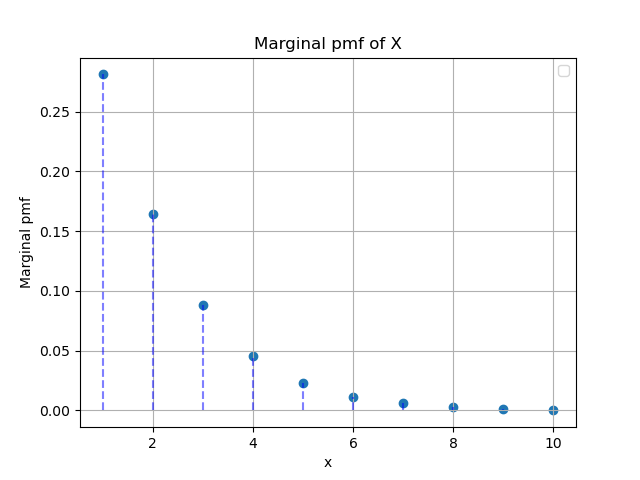
\includegraphics[width=\columnwidth]{/home/yogitha/47.2023/figs/pmfx.png}
\caption{Marginal pmf}
\label{fig:i_pmf}
\end{figure}
\end{enumerate}
Steps of simulation:
\begin{enumerate}
\item Define function p as $P\brak{x,y}=\frac{3}{2^{x+y+3}}$ in C and run a loop to sum the function p for all values of y except $x\neq y$, for each value of x.
\item Store values of marginal pmf for each value of x in a dat file 
\item Using plt.scatter function of python, plot the graph of Marginal pmf of X vs X.
The same can be used to plot marginal pmf of Y
\end{enumerate}

\item The frequencies for autosomal alleles $A$ and $a$ are $p = 0.5$ and $q = 0.5$,
respectively, where $A$ is dominant over $a$. Under the assumption of random
mating, the mating frequency among dominant parents is.\\
\hfill(GATE XL 2023)\\
\iffalse
\let\negmedspace\undefined
\let\negthickspace\undefined
\documentclass[journal,12pt,twocolumn]{IEEEtran}
\usepackage{cite}
\usepackage{amsmath,amssymb,amsfonts,amsthm}
\usepackage{algorithmic}
\usepackage{graphicx}
\usepackage{textcomp}
\usepackage{xcolor}
\usepackage{txfonts}
\usepackage{listings}
\usepackage{enumitem}
\usepackage{mathtools}
\usepackage{gensymb}
\usepackage[breaklinks=true]{hyperref}
\usepackage{tkz-euclide} % loads  TikZ and tkz-base
\usepackage{listings}
\usepackage{gvv}
\usepackage{float}  % To use the [H] placement specifier

%
%\usepackage{setspace}
%\usepackage{gensymb}
%\doublespacing
%\singlespacing

%\usepackage{graphicx}
%\usepackage{amssymb}
%\usepackage{relsize}
%\usepackage[cmex10]{amsmath}
%\usepackage{amsthm}
%\interdisplaylinepenalty=2500
%\savesymbol{iint}
%\usepackage{txfonts}
%\restoresymbol{TXF}{iint}
%\usepackage{wasysym}
%\usepackage{amsthm}
%\usepackage{iithtlc}
%\usepackage{mathrsfs}
%\usepackage{txfonts}
%\usepackage{stfloats}
%\usepackage{bm}
%\usepackage{cite}
%\usepackage{cases}
%\usepackage{subfig}
%\usepackage{xtab}
%\usepackage{longtable}
%\usepackage{multirow}
%\usepackage{algorithm}
%\usepackage{algpseudocode}
%\usepackage{enumitem}
%\usepackage{mathtools}
%\usepackage{tikz}
%\usepackage{circuitikz}
%\usepackage{verbatim}
%\usepackage{tfrupee}
%\usepackage{stmaryrd}
%\usetkzobj{all}
%    \usepackage{color}                                            %%
%    \usepackage{array}                                            %%
%    \usepackage{longtable}                                        %%
%    \usepackage{calc}                                             %%
%    \usepackage{multirow}                                         %%
%    \usepackage{hhline}                                           %%
%    \usepackage{ifthen}                                           %%
  %optionally (for landscape tables embedded in another document): %%
%    \usepackage{lscape}     
%\usepackage{multicol}
%\usepackage{chngcntr}
%\usepackage{enumerate}

%\usepackage{wasysym}
%\documentclass[conference]{IEEEtran}
%\IEEEoverridecommandlockouts
% The preceding line is only needed to identify funding in the first footnote. If that is unneeded, please comment it out.

\newtheorem{theorem}{Theorem}[section]
\newtheorem{problem}{Problem}
\newtheorem{proposition}{Proposition}[section]
\newtheorem{lemma}{Lemma}[section]
\newtheorem{corollary}[theorem]{Corollary}
\newtheorem{example}{Example}[section]
\newtheorem{definition}[problem]{Definition}
%\newtheorem{thm}{Theorem}[section] 
%\newtheorem{defn}[thm]{Definition}
%\newtheorem{algorithm}{Algorithm}[section]
%\newtheorem{cor}{Corollary}
\newcommand{\BEQA}{\begin{eqnarray}}
\newcommand{\EEQA}{\end{eqnarray}}
%\newcommand{\define}{\stackrel{\triangle}{=}}
\theoremstyle{remark}
\newtheorem{rem}{Remark}

%\bibliographystyle{ieeetr}
\begin{document}
%

\bibliographystyle{IEEEtran}


\vspace{3cm}

\title{
%	\logo{
	47
%	}
}
\author{ EE22BTECH11059% <-this % stops a space
}	
%\title{
%	\logo{Matrix Analysis through Octave}{\begin{center}\includegraphics[scale=.24]{tlc}\end{center}}{}{HAMDSP}
%}


% paper title
% can use linebreaks \\ within to get better formatting as desired
%\title{Matrix Analysis through Octave}
%
%
% author names and IEEE memberships
% note positions of commas and nonbreaking spaces ( ~ ) LaTeX will not break
% a structure at a ~ so this keeps an author's name from being broken across
% two lines.
% use \thanks{} to gain access to the first footnote area
% a separate \thanks must be used for each paragraph as LaTeX2e's \thanks
% was not built to handle multiple paragraphs
%

%\author{<-this % stops a space
%\thanks{}}
%}
% note the % following the last \IEEEmembership and also \thanks - 
% these prevent an unwanted space from occurring between the last author name
% and the end of the author line. i.e., if you had this:
% 
% \author{....lastname \thanks{...} \thanks{...} }
%                     ^------------^------------^----Do not want these spaces!
%
% a space would be appended to the last name and could cause every name on that
% line to be shifted left slightly. This is one of those "LaTeX things". For
% instance, "\textbf{A} \textbf{B}" will typeset as "A B" not "AB". To get
% "AB" then you have to do: "\textbf{A}\textbf{B}"
% \thanks is no different in this regard, so shield the last } of each \thanks
% that ends a line with a % and do not let a space in before the next \thanks.
% Spaces after \IEEEmembership other than the last one are OK (and needed) as
% you are supposed to have spaces between the names. For what it is worth,
% this is a minor point as most people would not even notice if the said evil
% space somehow managed to creep in.



% The paper headers
%\markboth{Journal of \LaTeX\ Class Files,~Vol.~6, No.~1, January~2007}%
%{Shell \MakeLowercase{\textit{et al.}}: Bare Demo of IEEEtran.cls for Journals}
% The only time the second header will appear is for the odd numbered pages
% after the title page when using the twoside option.
% 
% *** Note that you probably will NOT want to include the author's ***
% *** name in the headers of peer review papers.                   ***
% You can use \ifCLASSOPTIONpeerreview for conditional compilation here if
% you desire.




% If you want to put a publisher's ID mark on the page you can do it like
% this:
%\IEEEpubid{0000--0000/00\$00.00~\copyright~2007 IEEE}
% Remember, if you use this you must call \IEEEpubidadjcol in the second
% column for its text to clear the IEEEpubid mark.



% make the title area
\maketitle

\newpage

%\tableofcontents

\bigskip

\renewcommand{\thefigure}{\theenumi}
\renewcommand{\thetable}{\theenumi}
%\renewcommand{\theequation}{\theenumi}

%\begin{abstract}
%%\boldmath
%In this letter, an algorithm for evaluating the exact analytical bit error rate  (BER)  for the piecewise linear (PL) combiner for  multiple relays is presented. Previous results were available only for upto three relays. The algorithm is unique in the sense that  the actual mathematical expressions, that are prohibitively large, need not be explicitly obtained. The diversity gain due to multiple relays is shown through plots of the analytical BER, well supported by simulations. 
%
%\end{abstract}
% IEEEtran.cls defaults to using nonbold math in the Abstract.
% This preserves the distinction between vectors and scalars. However,
% if the journal you are submitting to favors bold math in the abstract,
% then you can use LaTeX's standard command \boldmath at the very start
% of the abstract to achieve this. Many IEEE journals frown on math
% in the abstract anyway.

% Note that keywords are not normally used for peerreview papers.
%\begin{IEEEkeywords}
%Cooperative diversity, decode and forward, piecewise linear
%\end{IEEEkeywords}



% For peer review papers, you can put extra information on the cover
% page as needed:
% \ifCLASSOPTIONpeerreview
% \begin{center} \bfseries EDICS Category: 3-BBND \end{center}
% \fi
%
% For peerreview papers, this IEEEtran command inserts a page break and
% creates the second title. It will be ignored for other modes.
%\IEEEpeerreviewmaketitle

%\documentclass{article}
%\usepackage{amsmath}
%\section*{ASSIGNMENT 1}
Let \brak{X,Y} have joint probability mass function 
\begin{align}
p\brak{x,y}=  
	\begin{cases}
        \frac{c}{2^{x+y+2}} & if x=0,1,2,... \, y=0,1,2,...; x\neq y \\
        0 & otherwise
        \end{cases} 
\end{align} 
Then which of the following is true?\\
\hfill (GATE ST 2023) \\
\begin{enumerate}
\item $c = \frac{1}{2}$
\item $c = \frac{1}{4}$
\item $c > 1$
\item $X$ and $Y$ are independent
\end{enumerate}
\fi
\solution
For p\brak{x,y} to be joint probability mass function
\begin{align}
\sum\limits^{\infty}_{y=-\infty}\sum\limits^{\infty}_{x=-\infty}p(x,y)&=1 \, \vert x \neq y\\
\sum\limits^{\infty}_{y=0}\sum\limits^{\infty}_{x=0}\frac{c}{2^{x+y+2}}- \sum\limits_{x=y} \frac{c}{2^{x+y+2}}&=1\\
\sum\limits^{\infty}_{y=0}\frac{c}{2^{y+2}} \sum\limits^{\infty}_{x=0} 2^{-x}- \frac{c}{4}\sum\limits^{\infty}_{x=0}\frac{1}{4^x}&=1\\
\sum\limits^{\infty}_{y=0}\frac{2c}{2^{y+2}}- \frac{c}{3}&=1\\
\frac{2c}{4}\sum\limits^{\infty}_{y=0}2^{-y}-\frac{c}{3}&=1\\
c-\frac{c}{3}&=1\\
c&=\frac{3}{2}
\end{align}
\begin{enumerate}
\item Marginal probability mass function of X
\begin{align}
p_X\brak{x}&=\sum\limits^{\infty}_{y=0}p\brak{x,y} \vert x \neq y\\
&=\sum\limits^{\infty}_{y=0}\frac{3}{2^{x+y+3}}- p_{XY}\brak{x,x}\\
&=\frac{3}{2^{x+3}}\sum\limits^{\infty}_{y=0}2^{-y}-\frac{3}{2^{2x+3}}\\
&=\frac{3}{2^{x+2}}-\frac{3}{2^{2x+3}}
\end{align}
\item Marginal cdf of X
\begin{align}
F_X\brak{x}&=\sum\limits^{x}_{i=0} p_X\brak{X \leq x}\\
&=\sum\limits^{x}_{i=0}\brak{\frac{3}{2^{x+2}}-\frac{3}{2^{2x+3}}}\\
&=1+\frac{1}{2^{x+2}}-\frac{3}{2^{2x+3}}
\end{align}
\item Marginal probability mass function of Y
\begin{align}
p_Y\brak{y}&=\sum\limits^{\infty}_{x=0}p\brak{x,y} \vert x \neq y\\
&=\sum\limits^{\infty}_{x=0}\frac{3}{2^{x+y+3}}- p_{XY}\brak{y,y}\\
&=\frac{3}{2^{y+3}}\sum\limits^{\infty}_{x=0}2^{-x}-\frac{3}{2^{2y+3}}\\
&=\frac{3}{2^{y+2}}-\frac{3}{2^{2y+3}}\\
\end{align}
\item Marginal cdf of Y
\begin{align}
F_Y\brak{y}&=\sum\limits^{y}_{i=0} p_Y\brak{Y \leq y}\\
&=\sum\limits^{y}_{i=0}\brak{\frac{3}{2^{y+2}}-\frac{3}{2^{2y+3}}}\\
&=1+\frac{1}{2^{y+2}}-\frac{3}{2^{2y+3}}
\end{align}
\item For X and Y to be independent,
\begin{align}
p\brak{x,y}&=p_X\brak{x} p_Y\brak{y}\\
p_X\brak{x} p_Y\brak{y}&=\brak{\frac{3}{2^{x+2}}-\frac{3}{2^{2x+3}}}\brak{\frac{3}{2^{y+2}}-\frac{3}{2^{2y+3}}}\\
p\brak{x,y} &\neq p_X\brak{x} p_Y\brak{y}
\end{align}
\end{enumerate}
Option \brak{4} is incorrect.\\
$\therefore$ Only option \brak{3} is correct. \\
Simulations:
\begin{enumerate}
\item Marginal pmf of X
\begin{figure}[H]
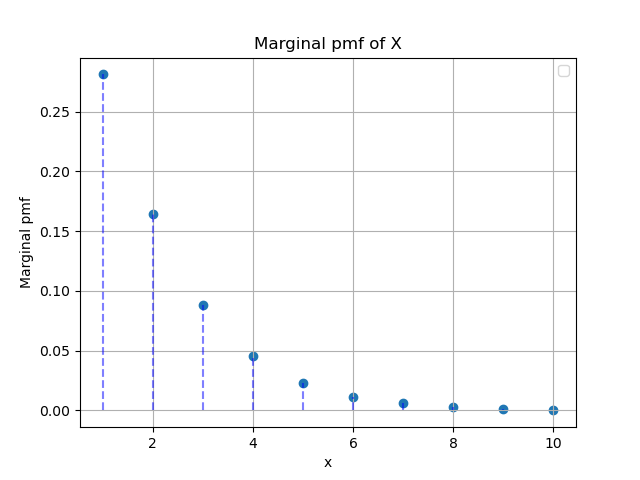
\includegraphics[width=\columnwidth]{/home/yogitha/47.2023/figs/pmfx.png}
\caption{Marginal pmf}
\label{fig:i_pmf}
\end{figure}
\end{enumerate}
Steps of simulation:
\begin{enumerate}
\item Define function p as $P\brak{x,y}=\frac{3}{2^{x+y+3}}$ in C and run a loop to sum the function p for all values of y except $x\neq y$, for each value of x.
\item Store values of marginal pmf for each value of x in a dat file 
\item Using plt.scatter function of python, plot the graph of Marginal pmf of X vs X.
The same can be used to plot marginal pmf of Y
\end{enumerate}

\item Let $X$ be a random variable having poisson distribution with mean $\lambda>0$. Then E\brak{\cond{\frac{1}{1+X}}{X>0}} equals
\begin{enumerate}
	\item $\frac{1-e^{-\lambda}-\lambda e^{-\lambda}}{\lambda\brak{1-e^{-\lambda}}}$
	\item $\frac{1-e^{-\lambda}}{\lambda}$
	\item $\frac{1-e^{-\lambda}-\lambda e^{-\lambda}}{\lambda}$
	\item $\frac{1-e^{-\lambda}}{\lambda +1}$
\end{enumerate}
\hfill(GATE ST 2023)\\
\solution\\
\iffalse
\let\negmedspace\undefined
\let\negthickspace\undefined
\documentclass[journal,12pt,twocolumn]{IEEEtran}
\usepackage{cite}
\usepackage{amsmath,amssymb,amsfonts,amsthm}
\usepackage{algorithmic}
\usepackage{graphicx}
\usepackage{textcomp}
\usepackage{xcolor}
\usepackage{txfonts}
\usepackage{listings}
\usepackage{enumitem}
\usepackage{mathtools}
\usepackage{gensymb}
\usepackage[breaklinks=true]{hyperref}
\usepackage{tkz-euclide} % loads  TikZ and tkz-base
\usepackage{listings}
\usepackage{gvv}
\usepackage{float}  % To use the [H] placement specifier

%
%\usepackage{setspace}
%\usepackage{gensymb}
%\doublespacing
%\singlespacing

%\usepackage{graphicx}
%\usepackage{amssymb}
%\usepackage{relsize}
%\usepackage[cmex10]{amsmath}
%\usepackage{amsthm}
%\interdisplaylinepenalty=2500
%\savesymbol{iint}
%\usepackage{txfonts}
%\restoresymbol{TXF}{iint}
%\usepackage{wasysym}
%\usepackage{amsthm}
%\usepackage{iithtlc}
%\usepackage{mathrsfs}
%\usepackage{txfonts}
%\usepackage{stfloats}
%\usepackage{bm}
%\usepackage{cite}
%\usepackage{cases}
%\usepackage{subfig}
%\usepackage{xtab}
%\usepackage{longtable}
%\usepackage{multirow}
%\usepackage{algorithm}
%\usepackage{algpseudocode}
%\usepackage{enumitem}
%\usepackage{mathtools}
%\usepackage{tikz}
%\usepackage{circuitikz}
%\usepackage{verbatim}
%\usepackage{tfrupee}
%\usepackage{stmaryrd}
%\usetkzobj{all}
%    \usepackage{color}                                            %%
%    \usepackage{array}                                            %%
%    \usepackage{longtable}                                        %%
%    \usepackage{calc}                                             %%
%    \usepackage{multirow}                                         %%
%    \usepackage{hhline}                                           %%
%    \usepackage{ifthen}                                           %%
  %optionally (for landscape tables embedded in another document): %%
%    \usepackage{lscape}     
%\usepackage{multicol}
%\usepackage{chngcntr}
%\usepackage{enumerate}

%\usepackage{wasysym}
%\documentclass[conference]{IEEEtran}
%\IEEEoverridecommandlockouts
% The preceding line is only needed to identify funding in the first footnote. If that is unneeded, please comment it out.

\newtheorem{theorem}{Theorem}[section]
\newtheorem{problem}{Problem}
\newtheorem{proposition}{Proposition}[section]
\newtheorem{lemma}{Lemma}[section]
\newtheorem{corollary}[theorem]{Corollary}
\newtheorem{example}{Example}[section]
\newtheorem{definition}[problem]{Definition}
%\newtheorem{thm}{Theorem}[section] 
%\newtheorem{defn}[thm]{Definition}
%\newtheorem{algorithm}{Algorithm}[section]
%\newtheorem{cor}{Corollary}
\newcommand{\BEQA}{\begin{eqnarray}}
\newcommand{\EEQA}{\end{eqnarray}}
%\newcommand{\define}{\stackrel{\triangle}{=}}
\theoremstyle{remark}
\newtheorem{rem}{Remark}

%\bibliographystyle{ieeetr}
\begin{document}
%

\bibliographystyle{IEEEtran}


\vspace{3cm}

\title{
%	\logo{
	47
%	}
}
\author{ EE22BTECH11059% <-this % stops a space
}	
%\title{
%	\logo{Matrix Analysis through Octave}{\begin{center}\includegraphics[scale=.24]{tlc}\end{center}}{}{HAMDSP}
%}


% paper title
% can use linebreaks \\ within to get better formatting as desired
%\title{Matrix Analysis through Octave}
%
%
% author names and IEEE memberships
% note positions of commas and nonbreaking spaces ( ~ ) LaTeX will not break
% a structure at a ~ so this keeps an author's name from being broken across
% two lines.
% use \thanks{} to gain access to the first footnote area
% a separate \thanks must be used for each paragraph as LaTeX2e's \thanks
% was not built to handle multiple paragraphs
%

%\author{<-this % stops a space
%\thanks{}}
%}
% note the % following the last \IEEEmembership and also \thanks - 
% these prevent an unwanted space from occurring between the last author name
% and the end of the author line. i.e., if you had this:
% 
% \author{....lastname \thanks{...} \thanks{...} }
%                     ^------------^------------^----Do not want these spaces!
%
% a space would be appended to the last name and could cause every name on that
% line to be shifted left slightly. This is one of those "LaTeX things". For
% instance, "\textbf{A} \textbf{B}" will typeset as "A B" not "AB". To get
% "AB" then you have to do: "\textbf{A}\textbf{B}"
% \thanks is no different in this regard, so shield the last } of each \thanks
% that ends a line with a % and do not let a space in before the next \thanks.
% Spaces after \IEEEmembership other than the last one are OK (and needed) as
% you are supposed to have spaces between the names. For what it is worth,
% this is a minor point as most people would not even notice if the said evil
% space somehow managed to creep in.



% The paper headers
%\markboth{Journal of \LaTeX\ Class Files,~Vol.~6, No.~1, January~2007}%
%{Shell \MakeLowercase{\textit{et al.}}: Bare Demo of IEEEtran.cls for Journals}
% The only time the second header will appear is for the odd numbered pages
% after the title page when using the twoside option.
% 
% *** Note that you probably will NOT want to include the author's ***
% *** name in the headers of peer review papers.                   ***
% You can use \ifCLASSOPTIONpeerreview for conditional compilation here if
% you desire.




% If you want to put a publisher's ID mark on the page you can do it like
% this:
%\IEEEpubid{0000--0000/00\$00.00~\copyright~2007 IEEE}
% Remember, if you use this you must call \IEEEpubidadjcol in the second
% column for its text to clear the IEEEpubid mark.



% make the title area
\maketitle

\newpage

%\tableofcontents

\bigskip

\renewcommand{\thefigure}{\theenumi}
\renewcommand{\thetable}{\theenumi}
%\renewcommand{\theequation}{\theenumi}

%\begin{abstract}
%%\boldmath
%In this letter, an algorithm for evaluating the exact analytical bit error rate  (BER)  for the piecewise linear (PL) combiner for  multiple relays is presented. Previous results were available only for upto three relays. The algorithm is unique in the sense that  the actual mathematical expressions, that are prohibitively large, need not be explicitly obtained. The diversity gain due to multiple relays is shown through plots of the analytical BER, well supported by simulations. 
%
%\end{abstract}
% IEEEtran.cls defaults to using nonbold math in the Abstract.
% This preserves the distinction between vectors and scalars. However,
% if the journal you are submitting to favors bold math in the abstract,
% then you can use LaTeX's standard command \boldmath at the very start
% of the abstract to achieve this. Many IEEE journals frown on math
% in the abstract anyway.

% Note that keywords are not normally used for peerreview papers.
%\begin{IEEEkeywords}
%Cooperative diversity, decode and forward, piecewise linear
%\end{IEEEkeywords}



% For peer review papers, you can put extra information on the cover
% page as needed:
% \ifCLASSOPTIONpeerreview
% \begin{center} \bfseries EDICS Category: 3-BBND \end{center}
% \fi
%
% For peerreview papers, this IEEEtran command inserts a page break and
% creates the second title. It will be ignored for other modes.
%\IEEEpeerreviewmaketitle

%\documentclass{article}
%\usepackage{amsmath}
%\section*{ASSIGNMENT 1}
Let \brak{X,Y} have joint probability mass function 
\begin{align}
p\brak{x,y}=  
	\begin{cases}
        \frac{c}{2^{x+y+2}} & if x=0,1,2,... \, y=0,1,2,...; x\neq y \\
        0 & otherwise
        \end{cases} 
\end{align} 
Then which of the following is true?\\
\hfill (GATE ST 2023) \\
\begin{enumerate}
\item $c = \frac{1}{2}$
\item $c = \frac{1}{4}$
\item $c > 1$
\item $X$ and $Y$ are independent
\end{enumerate}
\fi
\solution
For p\brak{x,y} to be joint probability mass function
\begin{align}
\sum\limits^{\infty}_{y=-\infty}\sum\limits^{\infty}_{x=-\infty}p(x,y)&=1 \, \vert x \neq y\\
\sum\limits^{\infty}_{y=0}\sum\limits^{\infty}_{x=0}\frac{c}{2^{x+y+2}}- \sum\limits_{x=y} \frac{c}{2^{x+y+2}}&=1\\
\sum\limits^{\infty}_{y=0}\frac{c}{2^{y+2}} \sum\limits^{\infty}_{x=0} 2^{-x}- \frac{c}{4}\sum\limits^{\infty}_{x=0}\frac{1}{4^x}&=1\\
\sum\limits^{\infty}_{y=0}\frac{2c}{2^{y+2}}- \frac{c}{3}&=1\\
\frac{2c}{4}\sum\limits^{\infty}_{y=0}2^{-y}-\frac{c}{3}&=1\\
c-\frac{c}{3}&=1\\
c&=\frac{3}{2}
\end{align}
\begin{enumerate}
\item Marginal probability mass function of X
\begin{align}
p_X\brak{x}&=\sum\limits^{\infty}_{y=0}p\brak{x,y} \vert x \neq y\\
&=\sum\limits^{\infty}_{y=0}\frac{3}{2^{x+y+3}}- p_{XY}\brak{x,x}\\
&=\frac{3}{2^{x+3}}\sum\limits^{\infty}_{y=0}2^{-y}-\frac{3}{2^{2x+3}}\\
&=\frac{3}{2^{x+2}}-\frac{3}{2^{2x+3}}
\end{align}
\item Marginal cdf of X
\begin{align}
F_X\brak{x}&=\sum\limits^{x}_{i=0} p_X\brak{X \leq x}\\
&=\sum\limits^{x}_{i=0}\brak{\frac{3}{2^{x+2}}-\frac{3}{2^{2x+3}}}\\
&=1+\frac{1}{2^{x+2}}-\frac{3}{2^{2x+3}}
\end{align}
\item Marginal probability mass function of Y
\begin{align}
p_Y\brak{y}&=\sum\limits^{\infty}_{x=0}p\brak{x,y} \vert x \neq y\\
&=\sum\limits^{\infty}_{x=0}\frac{3}{2^{x+y+3}}- p_{XY}\brak{y,y}\\
&=\frac{3}{2^{y+3}}\sum\limits^{\infty}_{x=0}2^{-x}-\frac{3}{2^{2y+3}}\\
&=\frac{3}{2^{y+2}}-\frac{3}{2^{2y+3}}\\
\end{align}
\item Marginal cdf of Y
\begin{align}
F_Y\brak{y}&=\sum\limits^{y}_{i=0} p_Y\brak{Y \leq y}\\
&=\sum\limits^{y}_{i=0}\brak{\frac{3}{2^{y+2}}-\frac{3}{2^{2y+3}}}\\
&=1+\frac{1}{2^{y+2}}-\frac{3}{2^{2y+3}}
\end{align}
\item For X and Y to be independent,
\begin{align}
p\brak{x,y}&=p_X\brak{x} p_Y\brak{y}\\
p_X\brak{x} p_Y\brak{y}&=\brak{\frac{3}{2^{x+2}}-\frac{3}{2^{2x+3}}}\brak{\frac{3}{2^{y+2}}-\frac{3}{2^{2y+3}}}\\
p\brak{x,y} &\neq p_X\brak{x} p_Y\brak{y}
\end{align}
\end{enumerate}
Option \brak{4} is incorrect.\\
$\therefore$ Only option \brak{3} is correct. \\
Simulations:
\begin{enumerate}
\item Marginal pmf of X
\begin{figure}[H]
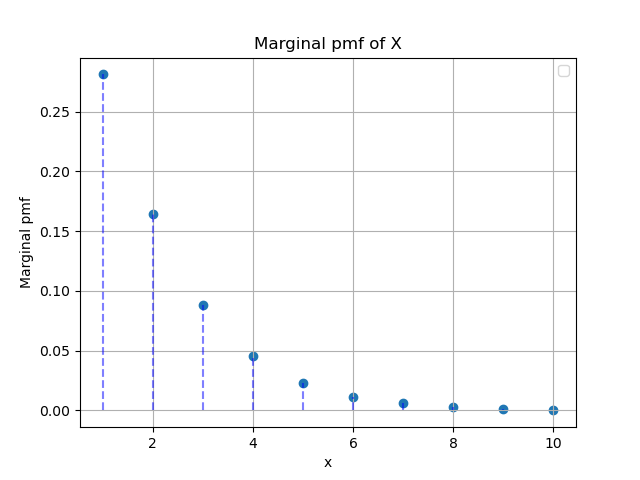
\includegraphics[width=\columnwidth]{/home/yogitha/47.2023/figs/pmfx.png}
\caption{Marginal pmf}
\label{fig:i_pmf}
\end{figure}
\end{enumerate}
Steps of simulation:
\begin{enumerate}
\item Define function p as $P\brak{x,y}=\frac{3}{2^{x+y+3}}$ in C and run a loop to sum the function p for all values of y except $x\neq y$, for each value of x.
\item Store values of marginal pmf for each value of x in a dat file 
\item Using plt.scatter function of python, plot the graph of Marginal pmf of X vs X.
The same can be used to plot marginal pmf of Y
\end{enumerate}

\item Consider the probability space $(\Omega, \mathcal{G}, P)$, where 
   $ \Omega = \{1, 2, 3, 4\}$, 
    $\mathcal{G} = \{\emptyset, \Omega, \{1\}, \{4\}, \{2, 3\}, \{1, 4\}, \{1, 2, 3\}, \{2, 3, 4\}\}$, 
    $P(\{1\}) = \frac{1}{4}$.
\item Let $X$ be the random variable defined on the above probability space as
   $ X(1) = 1$, 
    $X(2) = X(3) = 2$, 
    $X(4) = 3$.
If $P(X \leq 2) = \frac{3}{4}$, then find $P(\{1, 4\})$ (rounded off to two decimal places).\\\hfill (GATE ST 2023)\\
\iffalse
\documentclass[journal,11pt,onecolumn]{IEEEtran}
\usepackage{setspace}
\usepackage{gensymb}
\singlespacing
\usepackage[cmex10]{amsmath}
\usepackage{amsthm}
\usepackage{mathrsfs}
\usepackage{txfonts}
\usepackage{stfloats}
\usepackage{bm}
\usepackage{cite}
\usepackage{cases}
\usepackage{subfig}
\usepackage{longtable}
\usepackage{multirow}
\usepackage{enumitem}
\usepackage{mathtools}
\usepackage{tikz}
\usepackage{circuitikz}
\usepackage{verbatim}
\usepackage[breaklinks=true]{hyperref}
\usepackage{tkz-euclide} % loads  TikZ and tkz-base
\usepackage{listings}
\usepackage{color}    
\usepackage{array}    
\usepackage{longtable}
\usepackage{calc}     
\usepackage{multirow} 
\usepackage{hhline}   
\usepackage{ifthen}   
\usepackage{lscape}     
\usepackage{chngcntr}
\usepackage{float}
\DeclareMathOperator*{\Res}{Res}
\renewcommand\thesection{\arabic{section}}
\renewcommand\thesubsection{\thesection.\arabic{subsection}}
\renewcommand\thesubsubsection{\thesubsection.\arabic{subsubsection}}

\renewcommand\thesectiondis{\arabic{section}}
\renewcommand\thesubsectiondis{\thesectiondis.\arabic{subsection}}
\renewcommand\thesubsubsectiondis{\thesubsectiondis.\arabic{subsubsection}}
\renewcommand\thetable{\arabic{table}}
% correct bad hyphenation here
\hyphenation{op-tical net-works semi-conduc-tor}
\def\inputGnumericTable{}                                 %%

\lstset{
%language=C,
frame=single, 
breaklines=true,
columns=fullflexible
}
%\lstset{
%language=tex,
%frame=single, 
%breaklines=true
%}
\providecommand{\pr}[1]{\ensuremath{\Pr\left(#1\right)}}
\providecommand{\prt}[2]{\ensuremath{p_{#1}^{\left(#2\right)} }}        % own macro for this question
\providecommand{\qfunc}[1]{\ensuremath{Q\left(#1\right)}}
\providecommand{\sbrak}[1]{\ensuremath{{}\left[#1\right]}}
\providecommand{\lsbrak}[1]{\ensuremath{{}\left[#1\right.}}
\providecommand{\rsbrak}[1]{\ensuremath{{}\left.#1\right]}}
\providecommand{\brak}[1]{\ensuremath{\left(#1\right)}}
\providecommand{\lbrak}[1]{\ensuremath{\left(#1\right.}}
\providecommand{\rbrak}[1]{\ensuremath{\left.#1\right)}}
\providecommand{\cbrak}[1]{\ensuremath{\left\{#1\right\}}}
\providecommand{\lcbrak}[1]{\ensuremath{\left\{#1\right.}}
\providecommand{\rcbrak}[1]{\ensuremath{\left.#1\right\}}}
\newcommand{\sgn}{\mathop{\mathrm{sgn}}}
\providecommand{\abs}[1]{\left\vert#1\right\vert}
\providecommand{\res}[1]{\Res\displaylimits_{#1}} 
\providecommand{\norm}[1]{\left\lVert#1\right\rVert}
%\providecommand{\norm}[1]{\lVert#1\rVert}
\providecommand{\mtx}[1]{\mathbf{#1}}
\providecommand{\mean}[1]{E\left[ #1 \right]}
\providecommand{\cond}[2]{#1\middle|#2}
\providecommand{\fourier}{\overset{\mathcal{F}}{ \rightleftharpoons}}
%\providecommand{\hilbert}{\overset{\mathcal{H}}{ \rightleftharpoons}}
%\providecommand{\system}{\overset{\mathcal{H}}{ \longleftrightarrow}}
	%\newcommand{\solution}[2]{\textbf{Solution:}{#1}}
\newcommand{\solution}{\noindent \textbf{Solution: }}
\newcommand{\cosec}{\,\text{cosec}\,}
\providecommand{\dec}[2]{\ensuremath{\overset{#1}{\underset{#2}{\gtrless}}}}
\newcommand{\myvec}[1]{\ensuremath{\begin{pmatrix}#1\end{pmatrix}}}
\newcommand{\mydet}[1]{\ensuremath{\begin{vmatrix}#1\end{vmatrix}}}
\providecommand{\rank}{\text{rank}}
\providecommand{\pr}[1]{\ensuremath{\Pr\left(#1\right)}}
\providecommand{\qfunc}[1]{\ensuremath{Q\left(#1\right)}}
	\newcommand*{\permcomb}[4][0mu]{{{}^{#3}\mkern#1#2_{#4}}}
\newcommand*{\perm}[1][-3mu]{\permcomb[#1]{P}}
\newcommand*{\comb}[1][-1mu]{\permcomb[#1]{C}}
\providecommand{\qfunc}[1]{\ensuremath{Q\left(#1\right)}}
\providecommand{\gauss}[2]{\mathcal{N}\ensuremath{\left(#1,#2\right)}}
\providecommand{\diff}[2]{\ensuremath{\frac{d{#1}}{d{#2}}}}
\providecommand{\myceil}[1]{\left \lceil #1 \right \rceil }
\newcommand\figref{Fig.~\ref}
\newcommand\tabref{Table~\ref}
\newcommand{\sinc}{\,\text{sinc}\,}
\newcommand{\rect}{\,\text{rect}\,}
\title{Assignment}
\author{dushyant | EE22BTECH11031}
\begin{document}
\newtheorem{theorem}{Theorem}[section]
\newtheorem{problem}{Problem}
\newtheorem{proposition}{Proposition}[section]
\newtheorem{lemma}{Lemma}[section]
\newtheorem{corollary}[theorem]{Corollary}
\newtheorem{example}{Example}[section]
\newtheorem{definition}[problem]{Definition}
\newcommand{\BEQA}{\begin{eqnarray}}
\newcommand{\EEQA}{\end{eqnarray}}
\newcommand{\define}{\stackrel{\triangle}{=}}
\bibliographystyle{IEEEtran}
\providecommand{\mbf}{\mathbf}
\providecommand{\pr}[1]{\ensuremath{\Pr\left(#1\right)}}
\providecommand{\qfunc}[1]{\ensuremath{Q\left(#1\right)}}
\providecommand{\sbrak}[1]{\ensuremath{{}\left[#1\right]}}
\providecommand{\lsbrak}[1]{\ensuremath{{}\left[#1\right.}}
\providecommand{\rsbrak}[1]{\ensuremath{{}\left.#1\right]}}
\providecommand{\brak}[1]{\ensuremath{\left(#1\right)}}
\providecommand{\lbrak}[1]{\ensuremath{\left(#1\right.}}
\providecommand{\rbrak}[1]{\ensuremath{\left.#1\right)}}
\providecommand{\cbrak}[1]{\ensuremath{\left\{#1\right\}}}
\providecommand{\lcbrak}[1]{\ensuremath{\left\{#1\right.}}
\providecommand{\rcbrak}[1]{\ensuremath{\left.#1\right\}}}
\theoremstyle{remark}
\newtheorem{rem}{Remark}
\providecommand{\abs}[1]{\left\vert#1\right\vert}
\providecommand{\res}[1]{\Res\displaylimits_{#1}} 
\providecommand{\norm}[1]{\left\lVert#1\right\rVert}
\providecommand{\mtx}[1]{\mathbf{#1}}
\providecommand{\mean}[1]{E\left[ #1 \right]}
\providecommand{\fourier}{\overset{\mathcal{F}}{ \rightleftharpoons}}
\providecommand{\system}[1]{\overset{\mathcal{#1}}{ \longleftrightarrow}}
\providecommand{\dec}[2]{\ensuremath{\overset{#1}{\underset{#2}{\gtrless}}}}
\let\vec\mathbf
\def\putbox#1#2#3{\makebox[0in][l]{\makebox[#1][l]{}\raisebox{\baselineskip}[0in][0in]{\raisebox{#2}[0in][0in]{#3}}}}
     \def\rightbox#1{\makebox[0in][r]{#1}}
     \def\centbox#1{\makebox[0in]{#1}}
     \def\topbox#1{\raisebox{-\baselineskip}[0in][0in]{#1}}
     \def\midbox#1{\raisebox{-0.5\baselineskip}[0in][0in]{#1}}
\maketitle
\textbf{Question:}Consider the probability space $(\Omega, \mathcal{G}, P)$, where 
   $ \Omega = \{1, 2, 3, 4\}$, 
    $\mathcal{G} = \{\emptyset, \Omega, \{1\}, \{4\}, \{2, 3\}, \{1, 4\}, \{1, 2, 3\}, \{2, 3, 4\}\}$, 
    $P(\{1\}) = \frac{1}{4}$.
Let $X$ be the random variable defined on the above probability space as
   $ X(1) = 1$, 
    $X(2) = X(3) = 2$, 
    $X(4) = 3$.
If $P(X \leq 2) = \frac{3}{4}$, then find $P(\{1, 4\})$ (rounded off to two decimal places).\\\hfill (GATE ST 2023)\\
\fi
\solution
\begin{table}[ht]
\centering
\caption{Probablity space}
\label{tab:GATE ST 60-1}
\begin{tabular}{|c|c|c}
\hline
Probablity space &Value \\ \hline
$\Omega$ & $\{1, 2, 3, 4\}$\\\hline
$\mathcal{G}$ &$\{\emptyset, \Omega, \{1\}, \{4\}, \{2, 3\}, \{1, 4\}, \{1, 2, 3\}, \{2, 3, 4\}\}$\\\hline
$P(\{1\})$ &$\frac{1}{4}$\\\hline
$P(X \leq 2)$ & $\frac{3}{4}$\\\hline
\end{tabular}
\label{tab:gate/st/60-1}
\end{table}
\\
\begin{table}[ht]
\centering
\caption{Random variable}
    \label{tab:GATE ST 60-2}
\begin{tabular}{|c|c|c}
\hline
$X\brak{\Omega}$ & $\Omega$\\\hline
$\{1\}$ & 1\\\hline
$\{2,3\}$ &2\\\hline
$\{4\}$ & 3\\\hline
\end{tabular}
\label{tab:gate/st/60}
\end{table}
\\
Pmf is defined as\\
\begin{align}
p_x\brak{k} &= \begin{cases}
P(\{1\}) & ,k=1\\
P(\{2,3\}) &, k=2\\
P(\{4\}) &, k=3\\
\end{cases}
\end{align}
Values of P(\{2,3\}), P(\{4\}) are unknown, so let p, q be their respective values
\begin{align}
p_X\brak{k} &= \begin{cases}
\frac{1}{4} & ,k=1\\
p &, k=2\\
q &, k=3\\
\end{cases}
\end{align}
\begin{align}
\Pr{(\{1, 4\})} = p_X(1) +p_X(3)
\end{align}
We know\\
\begin{align}
p_X(1) +  p + q  &= 1
\end{align}
We can express Pr($X \leq 2$)as:
\begin{align}
\Pr{(X \leq 2)} &= p_X(1) + p\\
\end{align}
We can expres above equations as:
\begin{align}
\myvec{1 & 1
        \\1 & 0}\myvec{p \\q} = \myvec{\frac{3}{4}\\ \frac{1}{2}}
\end{align}
\begin{align}
p &= \frac{1}{2}, q =\frac{1}{4}
\end{align}
Finally
\begin{align}
\Pr{(\{1, 4\})} &= P(\{1\}) +q\\
\Pr{(\{1, 4\})} &= \frac{1}{4} + \frac{1}{4}\\
\Pr{(\{1, 4\})} &= 0.5
\end{align}
\begin{figure}[h]
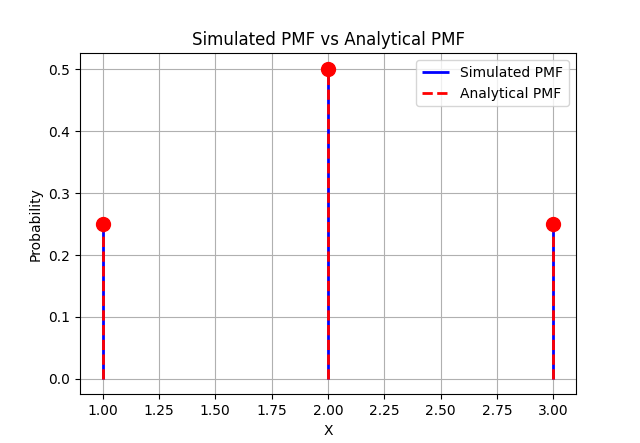
\includegraphics[width=\columnwidth]{figs/main2.png}
\caption{Analytical vs simulated}
\label{fig:GATE ST 60}
\end{figure}\\
Steps for simulating random variable.\\
\begin{enumerate}
\item Define the simulation size for datast (samples).
\item Assign calculated probablity for each probablity space p1, p2, p3, p4.
\item Define Random to generate a random number between 0 and 1.
\item Define the loop such that it generated number 1, 2, 3 for defined probablity space.
\item Store the simulated data in a .dat file.
\item Using matplotlib lib of python generate a V-line graph from the data in .dat file by counting the number of 1, 2, 3 .
\end{enumerate}

 

\item Let ${N(t)}_{t\ge 0}$ be a Poisson process with rate 1. Consider the following statements. 
\begin{enumerate}[label=(\alph*)]
\item $\pr{N(3)=3|N(5)=5}=\comb{5}{3}\left(\frac{3}{5}\right)^3 \left(\frac{2}{5}\right)^2$
\item If $S_5$ denotes the time of occurrence of the $5^{th}$ event for the above Poisson process,then $E(S_5|N(5)=3)=7$ \\
Which of the above statements is/are true?\\
\end{enumerate}
\begin{enumerate}[label=(\roman*)]
\item only (a)
\item only (b)
\item Both (a) and (b)
\item Neither (a) and (b)
\end{enumerate}
\hfill ( GATE ST 2023)\\
\solution \\
\iffalse
\let\negmedspace\undefined
\let\negthickspace\undefined
\documentclass[journal,12pt,twocolumn]{IEEEtran}
\usepackage{cite}
\usepackage{amsmath,amssymb,amsfonts,amsthm}
\usepackage{algorithmic}
\usepackage{graphicx}
\usepackage{textcomp}
\usepackage{xcolor}
\usepackage{txfonts}
\usepackage{listings}
\usepackage{enumitem}
\usepackage{mathtools}
\usepackage{gensymb}
\usepackage[breaklinks=true]{hyperref}
\usepackage{tkz-euclide} % loads  TikZ and tkz-base
\usepackage{listings}
\usepackage{gvv}
\usepackage{float}  % To use the [H] placement specifier

%
%\usepackage{setspace}
%\usepackage{gensymb}
%\doublespacing
%\singlespacing

%\usepackage{graphicx}
%\usepackage{amssymb}
%\usepackage{relsize}
%\usepackage[cmex10]{amsmath}
%\usepackage{amsthm}
%\interdisplaylinepenalty=2500
%\savesymbol{iint}
%\usepackage{txfonts}
%\restoresymbol{TXF}{iint}
%\usepackage{wasysym}
%\usepackage{amsthm}
%\usepackage{iithtlc}
%\usepackage{mathrsfs}
%\usepackage{txfonts}
%\usepackage{stfloats}
%\usepackage{bm}
%\usepackage{cite}
%\usepackage{cases}
%\usepackage{subfig}
%\usepackage{xtab}
%\usepackage{longtable}
%\usepackage{multirow}
%\usepackage{algorithm}
%\usepackage{algpseudocode}
%\usepackage{enumitem}
%\usepackage{mathtools}
%\usepackage{tikz}
%\usepackage{circuitikz}
%\usepackage{verbatim}
%\usepackage{tfrupee}
%\usepackage{stmaryrd}
%\usetkzobj{all}
%    \usepackage{color}                                            %%
%    \usepackage{array}                                            %%
%    \usepackage{longtable}                                        %%
%    \usepackage{calc}                                             %%
%    \usepackage{multirow}                                         %%
%    \usepackage{hhline}                                           %%
%    \usepackage{ifthen}                                           %%
  %optionally (for landscape tables embedded in another document): %%
%    \usepackage{lscape}     
%\usepackage{multicol}
%\usepackage{chngcntr}
%\usepackage{enumerate}

%\usepackage{wasysym}
%\documentclass[conference]{IEEEtran}
%\IEEEoverridecommandlockouts
% The preceding line is only needed to identify funding in the first footnote. If that is unneeded, please comment it out.

\newtheorem{theorem}{Theorem}[section]
\newtheorem{problem}{Problem}
\newtheorem{proposition}{Proposition}[section]
\newtheorem{lemma}{Lemma}[section]
\newtheorem{corollary}[theorem]{Corollary}
\newtheorem{example}{Example}[section]
\newtheorem{definition}[problem]{Definition}
%\newtheorem{thm}{Theorem}[section] 
%\newtheorem{defn}[thm]{Definition}
%\newtheorem{algorithm}{Algorithm}[section]
%\newtheorem{cor}{Corollary}
\newcommand{\BEQA}{\begin{eqnarray}}
\newcommand{\EEQA}{\end{eqnarray}}
%\newcommand{\define}{\stackrel{\triangle}{=}}
\theoremstyle{remark}
\newtheorem{rem}{Remark}

%\bibliographystyle{ieeetr}
\begin{document}
%

\bibliographystyle{IEEEtran}


\vspace{3cm}

\title{
%	\logo{
	47
%	}
}
\author{ EE22BTECH11059% <-this % stops a space
}	
%\title{
%	\logo{Matrix Analysis through Octave}{\begin{center}\includegraphics[scale=.24]{tlc}\end{center}}{}{HAMDSP}
%}


% paper title
% can use linebreaks \\ within to get better formatting as desired
%\title{Matrix Analysis through Octave}
%
%
% author names and IEEE memberships
% note positions of commas and nonbreaking spaces ( ~ ) LaTeX will not break
% a structure at a ~ so this keeps an author's name from being broken across
% two lines.
% use \thanks{} to gain access to the first footnote area
% a separate \thanks must be used for each paragraph as LaTeX2e's \thanks
% was not built to handle multiple paragraphs
%

%\author{<-this % stops a space
%\thanks{}}
%}
% note the % following the last \IEEEmembership and also \thanks - 
% these prevent an unwanted space from occurring between the last author name
% and the end of the author line. i.e., if you had this:
% 
% \author{....lastname \thanks{...} \thanks{...} }
%                     ^------------^------------^----Do not want these spaces!
%
% a space would be appended to the last name and could cause every name on that
% line to be shifted left slightly. This is one of those "LaTeX things". For
% instance, "\textbf{A} \textbf{B}" will typeset as "A B" not "AB". To get
% "AB" then you have to do: "\textbf{A}\textbf{B}"
% \thanks is no different in this regard, so shield the last } of each \thanks
% that ends a line with a % and do not let a space in before the next \thanks.
% Spaces after \IEEEmembership other than the last one are OK (and needed) as
% you are supposed to have spaces between the names. For what it is worth,
% this is a minor point as most people would not even notice if the said evil
% space somehow managed to creep in.



% The paper headers
%\markboth{Journal of \LaTeX\ Class Files,~Vol.~6, No.~1, January~2007}%
%{Shell \MakeLowercase{\textit{et al.}}: Bare Demo of IEEEtran.cls for Journals}
% The only time the second header will appear is for the odd numbered pages
% after the title page when using the twoside option.
% 
% *** Note that you probably will NOT want to include the author's ***
% *** name in the headers of peer review papers.                   ***
% You can use \ifCLASSOPTIONpeerreview for conditional compilation here if
% you desire.




% If you want to put a publisher's ID mark on the page you can do it like
% this:
%\IEEEpubid{0000--0000/00\$00.00~\copyright~2007 IEEE}
% Remember, if you use this you must call \IEEEpubidadjcol in the second
% column for its text to clear the IEEEpubid mark.



% make the title area
\maketitle

\newpage

%\tableofcontents

\bigskip

\renewcommand{\thefigure}{\theenumi}
\renewcommand{\thetable}{\theenumi}
%\renewcommand{\theequation}{\theenumi}

%\begin{abstract}
%%\boldmath
%In this letter, an algorithm for evaluating the exact analytical bit error rate  (BER)  for the piecewise linear (PL) combiner for  multiple relays is presented. Previous results were available only for upto three relays. The algorithm is unique in the sense that  the actual mathematical expressions, that are prohibitively large, need not be explicitly obtained. The diversity gain due to multiple relays is shown through plots of the analytical BER, well supported by simulations. 
%
%\end{abstract}
% IEEEtran.cls defaults to using nonbold math in the Abstract.
% This preserves the distinction between vectors and scalars. However,
% if the journal you are submitting to favors bold math in the abstract,
% then you can use LaTeX's standard command \boldmath at the very start
% of the abstract to achieve this. Many IEEE journals frown on math
% in the abstract anyway.

% Note that keywords are not normally used for peerreview papers.
%\begin{IEEEkeywords}
%Cooperative diversity, decode and forward, piecewise linear
%\end{IEEEkeywords}



% For peer review papers, you can put extra information on the cover
% page as needed:
% \ifCLASSOPTIONpeerreview
% \begin{center} \bfseries EDICS Category: 3-BBND \end{center}
% \fi
%
% For peerreview papers, this IEEEtran command inserts a page break and
% creates the second title. It will be ignored for other modes.
%\IEEEpeerreviewmaketitle

%\documentclass{article}
%\usepackage{amsmath}
%\section*{ASSIGNMENT 1}
Let \brak{X,Y} have joint probability mass function 
\begin{align}
p\brak{x,y}=  
	\begin{cases}
        \frac{c}{2^{x+y+2}} & if x=0,1,2,... \, y=0,1,2,...; x\neq y \\
        0 & otherwise
        \end{cases} 
\end{align} 
Then which of the following is true?\\
\hfill (GATE ST 2023) \\
\begin{enumerate}
\item $c = \frac{1}{2}$
\item $c = \frac{1}{4}$
\item $c > 1$
\item $X$ and $Y$ are independent
\end{enumerate}
\fi
\solution
For p\brak{x,y} to be joint probability mass function
\begin{align}
\sum\limits^{\infty}_{y=-\infty}\sum\limits^{\infty}_{x=-\infty}p(x,y)&=1 \, \vert x \neq y\\
\sum\limits^{\infty}_{y=0}\sum\limits^{\infty}_{x=0}\frac{c}{2^{x+y+2}}- \sum\limits_{x=y} \frac{c}{2^{x+y+2}}&=1\\
\sum\limits^{\infty}_{y=0}\frac{c}{2^{y+2}} \sum\limits^{\infty}_{x=0} 2^{-x}- \frac{c}{4}\sum\limits^{\infty}_{x=0}\frac{1}{4^x}&=1\\
\sum\limits^{\infty}_{y=0}\frac{2c}{2^{y+2}}- \frac{c}{3}&=1\\
\frac{2c}{4}\sum\limits^{\infty}_{y=0}2^{-y}-\frac{c}{3}&=1\\
c-\frac{c}{3}&=1\\
c&=\frac{3}{2}
\end{align}
\begin{enumerate}
\item Marginal probability mass function of X
\begin{align}
p_X\brak{x}&=\sum\limits^{\infty}_{y=0}p\brak{x,y} \vert x \neq y\\
&=\sum\limits^{\infty}_{y=0}\frac{3}{2^{x+y+3}}- p_{XY}\brak{x,x}\\
&=\frac{3}{2^{x+3}}\sum\limits^{\infty}_{y=0}2^{-y}-\frac{3}{2^{2x+3}}\\
&=\frac{3}{2^{x+2}}-\frac{3}{2^{2x+3}}
\end{align}
\item Marginal cdf of X
\begin{align}
F_X\brak{x}&=\sum\limits^{x}_{i=0} p_X\brak{X \leq x}\\
&=\sum\limits^{x}_{i=0}\brak{\frac{3}{2^{x+2}}-\frac{3}{2^{2x+3}}}\\
&=1+\frac{1}{2^{x+2}}-\frac{3}{2^{2x+3}}
\end{align}
\item Marginal probability mass function of Y
\begin{align}
p_Y\brak{y}&=\sum\limits^{\infty}_{x=0}p\brak{x,y} \vert x \neq y\\
&=\sum\limits^{\infty}_{x=0}\frac{3}{2^{x+y+3}}- p_{XY}\brak{y,y}\\
&=\frac{3}{2^{y+3}}\sum\limits^{\infty}_{x=0}2^{-x}-\frac{3}{2^{2y+3}}\\
&=\frac{3}{2^{y+2}}-\frac{3}{2^{2y+3}}\\
\end{align}
\item Marginal cdf of Y
\begin{align}
F_Y\brak{y}&=\sum\limits^{y}_{i=0} p_Y\brak{Y \leq y}\\
&=\sum\limits^{y}_{i=0}\brak{\frac{3}{2^{y+2}}-\frac{3}{2^{2y+3}}}\\
&=1+\frac{1}{2^{y+2}}-\frac{3}{2^{2y+3}}
\end{align}
\item For X and Y to be independent,
\begin{align}
p\brak{x,y}&=p_X\brak{x} p_Y\brak{y}\\
p_X\brak{x} p_Y\brak{y}&=\brak{\frac{3}{2^{x+2}}-\frac{3}{2^{2x+3}}}\brak{\frac{3}{2^{y+2}}-\frac{3}{2^{2y+3}}}\\
p\brak{x,y} &\neq p_X\brak{x} p_Y\brak{y}
\end{align}
\end{enumerate}
Option \brak{4} is incorrect.\\
$\therefore$ Only option \brak{3} is correct. \\
Simulations:
\begin{enumerate}
\item Marginal pmf of X
\begin{figure}[H]
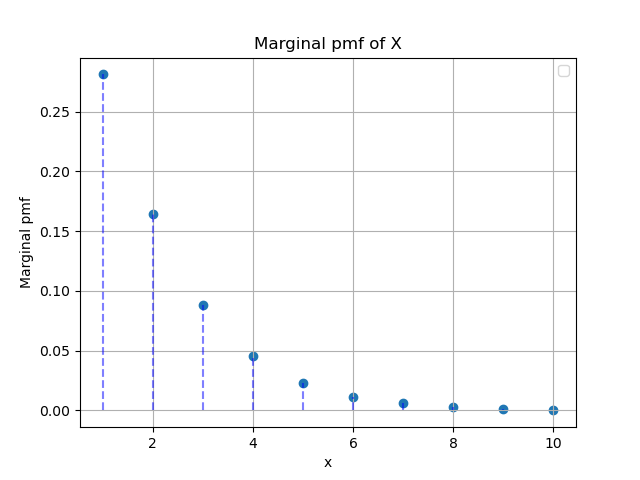
\includegraphics[width=\columnwidth]{/home/yogitha/47.2023/figs/pmfx.png}
\caption{Marginal pmf}
\label{fig:i_pmf}
\end{figure}
\end{enumerate}
Steps of simulation:
\begin{enumerate}
\item Define function p as $P\brak{x,y}=\frac{3}{2^{x+y+3}}$ in C and run a loop to sum the function p for all values of y except $x\neq y$, for each value of x.
\item Store values of marginal pmf for each value of x in a dat file 
\item Using plt.scatter function of python, plot the graph of Marginal pmf of X vs X.
The same can be used to plot marginal pmf of Y
\end{enumerate}

\item Suppose that $\vec{X_1}, \vec{X_2},\ldots, \vec{X_n}, \vec{Y_1}, \vec{Y_2},\ldots, \vec{Y_n}$ are independent and identically distributed random vectors each having $N_p\brak{\bm{\mu},\Sigma}$ distributions, where $\Sigma$ is non-singular, $p>1$ and $n>1$. If $\vec{X} = \frac{1}{n}\sum_{i=1}^{n}\vec{X_i}$ and $\vec{Y} = \frac{1}{n}\sum_{i=1}^{n}\vec{Y_i}$, then which one of the following statements is true?
\begin{enumerate}[label=(\alph*)]
\item There exists $c>0$ such that $c{\brak{\vec{X}-\bm{\mu}}}^T{\Sigma}^{-1}\brak{\vec{X}-\bm{\mu}}$ has ${\chi}^2$-distribution with $p$ degrees of freedom.
\item There exists $c>0$ such that $c{\brak{\vec{X}-\vec{Y}}^T}{\Sigma}^{-1}\brak{\vec{X}-\vec{Y}}$ has ${\chi}^2$-distribution with $\brak{p-1}$ degrees of freedom.
\item There exists $c>0$ such that $c\sum_{i=1}^n{\brak{\vec{X_i}-\vec{X}}}^T{\Sigma}^{-1}\brak{\vec{X_i}-\vec{X}}$ has ${\chi}^2$-distribution with $p$ degrees of freedom.
\item There exists $c>0$ such that $c\sum_{i=1}^n{\brak{\vec{X_i}-\vec{Y_i}-\vec{X}+\vec{Y}}}^T{\Sigma}^{-1}\brak{\vec{X_i}-\vec{Y_i}-\vec{X}+\vec{Y}}$ has ${\chi}^2$-distribution with $p$ degrees of freedom.   \hfill{GATE ST Paper 2023} 
\end{enumerate} 
\input{2023/ST/25/assignment11.tex}
\item In a locality 'A', the probability of a convective storm event is $0.7$ with a density function,
\begin{align}
f_{X_1}\brak{x_1} = e^{-x_1},\quad x_1>0
\end{align} 
The probability of tropical cyclone-induced storm in the same location is given by the density function,
\begin{align}
f_{X_2}\brak{x_2} = 2e^{-2x_2},\quad x_2>0
\end{align}
The probability of occuring more than 1 unit of storm event is\\
\hfill(GATE AG 2023)\\
\iffalse
\let\negmedspace\undefined
\let\negthickspace\undefined
\documentclass[journal,12pt,twocolumn]{IEEEtran}
\usepackage{cite}
\usepackage{amsmath,amssymb,amsfonts,amsthm}
\usepackage{algorithmic}
\usepackage{graphicx}
\usepackage{textcomp}
\usepackage{xcolor}
\usepackage{txfonts}
\usepackage{listings}
\usepackage{enumitem}
\usepackage{mathtools}
\usepackage{gensymb}
\usepackage[breaklinks=true]{hyperref}
\usepackage{tkz-euclide} % loads  TikZ and tkz-base
\usepackage{listings}
\usepackage{gvv}
\usepackage{float}  % To use the [H] placement specifier

%
%\usepackage{setspace}
%\usepackage{gensymb}
%\doublespacing
%\singlespacing

%\usepackage{graphicx}
%\usepackage{amssymb}
%\usepackage{relsize}
%\usepackage[cmex10]{amsmath}
%\usepackage{amsthm}
%\interdisplaylinepenalty=2500
%\savesymbol{iint}
%\usepackage{txfonts}
%\restoresymbol{TXF}{iint}
%\usepackage{wasysym}
%\usepackage{amsthm}
%\usepackage{iithtlc}
%\usepackage{mathrsfs}
%\usepackage{txfonts}
%\usepackage{stfloats}
%\usepackage{bm}
%\usepackage{cite}
%\usepackage{cases}
%\usepackage{subfig}
%\usepackage{xtab}
%\usepackage{longtable}
%\usepackage{multirow}
%\usepackage{algorithm}
%\usepackage{algpseudocode}
%\usepackage{enumitem}
%\usepackage{mathtools}
%\usepackage{tikz}
%\usepackage{circuitikz}
%\usepackage{verbatim}
%\usepackage{tfrupee}
%\usepackage{stmaryrd}
%\usetkzobj{all}
%    \usepackage{color}                                            %%
%    \usepackage{array}                                            %%
%    \usepackage{longtable}                                        %%
%    \usepackage{calc}                                             %%
%    \usepackage{multirow}                                         %%
%    \usepackage{hhline}                                           %%
%    \usepackage{ifthen}                                           %%
  %optionally (for landscape tables embedded in another document): %%
%    \usepackage{lscape}     
%\usepackage{multicol}
%\usepackage{chngcntr}
%\usepackage{enumerate}

%\usepackage{wasysym}
%\documentclass[conference]{IEEEtran}
%\IEEEoverridecommandlockouts
% The preceding line is only needed to identify funding in the first footnote. If that is unneeded, please comment it out.

\newtheorem{theorem}{Theorem}[section]
\newtheorem{problem}{Problem}
\newtheorem{proposition}{Proposition}[section]
\newtheorem{lemma}{Lemma}[section]
\newtheorem{corollary}[theorem]{Corollary}
\newtheorem{example}{Example}[section]
\newtheorem{definition}[problem]{Definition}
%\newtheorem{thm}{Theorem}[section] 
%\newtheorem{defn}[thm]{Definition}
%\newtheorem{algorithm}{Algorithm}[section]
%\newtheorem{cor}{Corollary}
\newcommand{\BEQA}{\begin{eqnarray}}
\newcommand{\EEQA}{\end{eqnarray}}
%\newcommand{\define}{\stackrel{\triangle}{=}}
\theoremstyle{remark}
\newtheorem{rem}{Remark}

%\bibliographystyle{ieeetr}
\begin{document}
%

\bibliographystyle{IEEEtran}


\vspace{3cm}

\title{
%	\logo{
	47
%	}
}
\author{ EE22BTECH11059% <-this % stops a space
}	
%\title{
%	\logo{Matrix Analysis through Octave}{\begin{center}\includegraphics[scale=.24]{tlc}\end{center}}{}{HAMDSP}
%}


% paper title
% can use linebreaks \\ within to get better formatting as desired
%\title{Matrix Analysis through Octave}
%
%
% author names and IEEE memberships
% note positions of commas and nonbreaking spaces ( ~ ) LaTeX will not break
% a structure at a ~ so this keeps an author's name from being broken across
% two lines.
% use \thanks{} to gain access to the first footnote area
% a separate \thanks must be used for each paragraph as LaTeX2e's \thanks
% was not built to handle multiple paragraphs
%

%\author{<-this % stops a space
%\thanks{}}
%}
% note the % following the last \IEEEmembership and also \thanks - 
% these prevent an unwanted space from occurring between the last author name
% and the end of the author line. i.e., if you had this:
% 
% \author{....lastname \thanks{...} \thanks{...} }
%                     ^------------^------------^----Do not want these spaces!
%
% a space would be appended to the last name and could cause every name on that
% line to be shifted left slightly. This is one of those "LaTeX things". For
% instance, "\textbf{A} \textbf{B}" will typeset as "A B" not "AB". To get
% "AB" then you have to do: "\textbf{A}\textbf{B}"
% \thanks is no different in this regard, so shield the last } of each \thanks
% that ends a line with a % and do not let a space in before the next \thanks.
% Spaces after \IEEEmembership other than the last one are OK (and needed) as
% you are supposed to have spaces between the names. For what it is worth,
% this is a minor point as most people would not even notice if the said evil
% space somehow managed to creep in.



% The paper headers
%\markboth{Journal of \LaTeX\ Class Files,~Vol.~6, No.~1, January~2007}%
%{Shell \MakeLowercase{\textit{et al.}}: Bare Demo of IEEEtran.cls for Journals}
% The only time the second header will appear is for the odd numbered pages
% after the title page when using the twoside option.
% 
% *** Note that you probably will NOT want to include the author's ***
% *** name in the headers of peer review papers.                   ***
% You can use \ifCLASSOPTIONpeerreview for conditional compilation here if
% you desire.




% If you want to put a publisher's ID mark on the page you can do it like
% this:
%\IEEEpubid{0000--0000/00\$00.00~\copyright~2007 IEEE}
% Remember, if you use this you must call \IEEEpubidadjcol in the second
% column for its text to clear the IEEEpubid mark.



% make the title area
\maketitle

\newpage

%\tableofcontents

\bigskip

\renewcommand{\thefigure}{\theenumi}
\renewcommand{\thetable}{\theenumi}
%\renewcommand{\theequation}{\theenumi}

%\begin{abstract}
%%\boldmath
%In this letter, an algorithm for evaluating the exact analytical bit error rate  (BER)  for the piecewise linear (PL) combiner for  multiple relays is presented. Previous results were available only for upto three relays. The algorithm is unique in the sense that  the actual mathematical expressions, that are prohibitively large, need not be explicitly obtained. The diversity gain due to multiple relays is shown through plots of the analytical BER, well supported by simulations. 
%
%\end{abstract}
% IEEEtran.cls defaults to using nonbold math in the Abstract.
% This preserves the distinction between vectors and scalars. However,
% if the journal you are submitting to favors bold math in the abstract,
% then you can use LaTeX's standard command \boldmath at the very start
% of the abstract to achieve this. Many IEEE journals frown on math
% in the abstract anyway.

% Note that keywords are not normally used for peerreview papers.
%\begin{IEEEkeywords}
%Cooperative diversity, decode and forward, piecewise linear
%\end{IEEEkeywords}



% For peer review papers, you can put extra information on the cover
% page as needed:
% \ifCLASSOPTIONpeerreview
% \begin{center} \bfseries EDICS Category: 3-BBND \end{center}
% \fi
%
% For peerreview papers, this IEEEtran command inserts a page break and
% creates the second title. It will be ignored for other modes.
%\IEEEpeerreviewmaketitle

%\documentclass{article}
%\usepackage{amsmath}
%\section*{ASSIGNMENT 1}
Let \brak{X,Y} have joint probability mass function 
\begin{align}
p\brak{x,y}=  
	\begin{cases}
        \frac{c}{2^{x+y+2}} & if x=0,1,2,... \, y=0,1,2,...; x\neq y \\
        0 & otherwise
        \end{cases} 
\end{align} 
Then which of the following is true?\\
\hfill (GATE ST 2023) \\
\begin{enumerate}
\item $c = \frac{1}{2}$
\item $c = \frac{1}{4}$
\item $c > 1$
\item $X$ and $Y$ are independent
\end{enumerate}
\fi
\solution
For p\brak{x,y} to be joint probability mass function
\begin{align}
\sum\limits^{\infty}_{y=-\infty}\sum\limits^{\infty}_{x=-\infty}p(x,y)&=1 \, \vert x \neq y\\
\sum\limits^{\infty}_{y=0}\sum\limits^{\infty}_{x=0}\frac{c}{2^{x+y+2}}- \sum\limits_{x=y} \frac{c}{2^{x+y+2}}&=1\\
\sum\limits^{\infty}_{y=0}\frac{c}{2^{y+2}} \sum\limits^{\infty}_{x=0} 2^{-x}- \frac{c}{4}\sum\limits^{\infty}_{x=0}\frac{1}{4^x}&=1\\
\sum\limits^{\infty}_{y=0}\frac{2c}{2^{y+2}}- \frac{c}{3}&=1\\
\frac{2c}{4}\sum\limits^{\infty}_{y=0}2^{-y}-\frac{c}{3}&=1\\
c-\frac{c}{3}&=1\\
c&=\frac{3}{2}
\end{align}
\begin{enumerate}
\item Marginal probability mass function of X
\begin{align}
p_X\brak{x}&=\sum\limits^{\infty}_{y=0}p\brak{x,y} \vert x \neq y\\
&=\sum\limits^{\infty}_{y=0}\frac{3}{2^{x+y+3}}- p_{XY}\brak{x,x}\\
&=\frac{3}{2^{x+3}}\sum\limits^{\infty}_{y=0}2^{-y}-\frac{3}{2^{2x+3}}\\
&=\frac{3}{2^{x+2}}-\frac{3}{2^{2x+3}}
\end{align}
\item Marginal cdf of X
\begin{align}
F_X\brak{x}&=\sum\limits^{x}_{i=0} p_X\brak{X \leq x}\\
&=\sum\limits^{x}_{i=0}\brak{\frac{3}{2^{x+2}}-\frac{3}{2^{2x+3}}}\\
&=1+\frac{1}{2^{x+2}}-\frac{3}{2^{2x+3}}
\end{align}
\item Marginal probability mass function of Y
\begin{align}
p_Y\brak{y}&=\sum\limits^{\infty}_{x=0}p\brak{x,y} \vert x \neq y\\
&=\sum\limits^{\infty}_{x=0}\frac{3}{2^{x+y+3}}- p_{XY}\brak{y,y}\\
&=\frac{3}{2^{y+3}}\sum\limits^{\infty}_{x=0}2^{-x}-\frac{3}{2^{2y+3}}\\
&=\frac{3}{2^{y+2}}-\frac{3}{2^{2y+3}}\\
\end{align}
\item Marginal cdf of Y
\begin{align}
F_Y\brak{y}&=\sum\limits^{y}_{i=0} p_Y\brak{Y \leq y}\\
&=\sum\limits^{y}_{i=0}\brak{\frac{3}{2^{y+2}}-\frac{3}{2^{2y+3}}}\\
&=1+\frac{1}{2^{y+2}}-\frac{3}{2^{2y+3}}
\end{align}
\item For X and Y to be independent,
\begin{align}
p\brak{x,y}&=p_X\brak{x} p_Y\brak{y}\\
p_X\brak{x} p_Y\brak{y}&=\brak{\frac{3}{2^{x+2}}-\frac{3}{2^{2x+3}}}\brak{\frac{3}{2^{y+2}}-\frac{3}{2^{2y+3}}}\\
p\brak{x,y} &\neq p_X\brak{x} p_Y\brak{y}
\end{align}
\end{enumerate}
Option \brak{4} is incorrect.\\
$\therefore$ Only option \brak{3} is correct. \\
Simulations:
\begin{enumerate}
\item Marginal pmf of X
\begin{figure}[H]
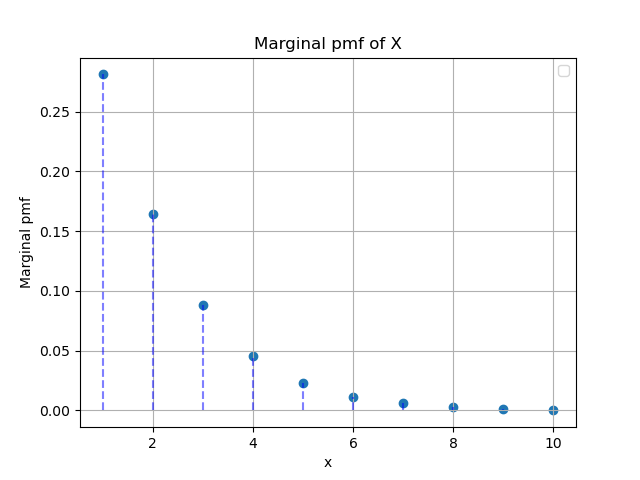
\includegraphics[width=\columnwidth]{/home/yogitha/47.2023/figs/pmfx.png}
\caption{Marginal pmf}
\label{fig:i_pmf}
\end{figure}
\end{enumerate}
Steps of simulation:
\begin{enumerate}
\item Define function p as $P\brak{x,y}=\frac{3}{2^{x+y+3}}$ in C and run a loop to sum the function p for all values of y except $x\neq y$, for each value of x.
\item Store values of marginal pmf for each value of x in a dat file 
\item Using plt.scatter function of python, plot the graph of Marginal pmf of X vs X.
The same can be used to plot marginal pmf of Y
\end{enumerate}

\item Suppose that $X$ is a discrete random variable with the following probability mass
\begin{align}
	P(X=0)&=\frac{1}{2}\brak{1+e^{-1}}\\
	P(X=k)&=\frac{e^{-1}}{2k!} \; for \; k=1,2,3,... \, .
\end{align}
Which of the following is/are true?
\begin{enumerate}
	\item $E(X)=1$
	\item $E(X)<1$
	\item $E(X|X>0)<\frac{1}{2}$
	\item $E(X|X>0)>\frac{1}{2}$
\end{enumerate}
\hfill (GATE ST 2023)\\
\iffalse
\let\negmedspace\undefined
\let\negthickspace\undefined
\documentclass[journal,12pt,twocolumn]{IEEEtran}
\usepackage{cite}
\usepackage{amsmath,amssymb,amsfonts,amsthm}
\usepackage{algorithmic}
\usepackage{graphicx}
\usepackage{textcomp}
\usepackage{xcolor}
\usepackage{txfonts}
\usepackage{listings}
\usepackage{enumitem}
\usepackage{mathtools}
\usepackage{gensymb}
\usepackage[breaklinks=true]{hyperref}
\usepackage{tkz-euclide} % loads  TikZ and tkz-base
\usepackage{listings}
\usepackage{gvv}
\usepackage{float}  % To use the [H] placement specifier

%
%\usepackage{setspace}
%\usepackage{gensymb}
%\doublespacing
%\singlespacing

%\usepackage{graphicx}
%\usepackage{amssymb}
%\usepackage{relsize}
%\usepackage[cmex10]{amsmath}
%\usepackage{amsthm}
%\interdisplaylinepenalty=2500
%\savesymbol{iint}
%\usepackage{txfonts}
%\restoresymbol{TXF}{iint}
%\usepackage{wasysym}
%\usepackage{amsthm}
%\usepackage{iithtlc}
%\usepackage{mathrsfs}
%\usepackage{txfonts}
%\usepackage{stfloats}
%\usepackage{bm}
%\usepackage{cite}
%\usepackage{cases}
%\usepackage{subfig}
%\usepackage{xtab}
%\usepackage{longtable}
%\usepackage{multirow}
%\usepackage{algorithm}
%\usepackage{algpseudocode}
%\usepackage{enumitem}
%\usepackage{mathtools}
%\usepackage{tikz}
%\usepackage{circuitikz}
%\usepackage{verbatim}
%\usepackage{tfrupee}
%\usepackage{stmaryrd}
%\usetkzobj{all}
%    \usepackage{color}                                            %%
%    \usepackage{array}                                            %%
%    \usepackage{longtable}                                        %%
%    \usepackage{calc}                                             %%
%    \usepackage{multirow}                                         %%
%    \usepackage{hhline}                                           %%
%    \usepackage{ifthen}                                           %%
  %optionally (for landscape tables embedded in another document): %%
%    \usepackage{lscape}     
%\usepackage{multicol}
%\usepackage{chngcntr}
%\usepackage{enumerate}

%\usepackage{wasysym}
%\documentclass[conference]{IEEEtran}
%\IEEEoverridecommandlockouts
% The preceding line is only needed to identify funding in the first footnote. If that is unneeded, please comment it out.

\newtheorem{theorem}{Theorem}[section]
\newtheorem{problem}{Problem}
\newtheorem{proposition}{Proposition}[section]
\newtheorem{lemma}{Lemma}[section]
\newtheorem{corollary}[theorem]{Corollary}
\newtheorem{example}{Example}[section]
\newtheorem{definition}[problem]{Definition}
%\newtheorem{thm}{Theorem}[section] 
%\newtheorem{defn}[thm]{Definition}
%\newtheorem{algorithm}{Algorithm}[section]
%\newtheorem{cor}{Corollary}
\newcommand{\BEQA}{\begin{eqnarray}}
\newcommand{\EEQA}{\end{eqnarray}}
%\newcommand{\define}{\stackrel{\triangle}{=}}
\theoremstyle{remark}
\newtheorem{rem}{Remark}

%\bibliographystyle{ieeetr}
\begin{document}
%

\bibliographystyle{IEEEtran}


\vspace{3cm}

\title{
%	\logo{
	47
%	}
}
\author{ EE22BTECH11059% <-this % stops a space
}	
%\title{
%	\logo{Matrix Analysis through Octave}{\begin{center}\includegraphics[scale=.24]{tlc}\end{center}}{}{HAMDSP}
%}


% paper title
% can use linebreaks \\ within to get better formatting as desired
%\title{Matrix Analysis through Octave}
%
%
% author names and IEEE memberships
% note positions of commas and nonbreaking spaces ( ~ ) LaTeX will not break
% a structure at a ~ so this keeps an author's name from being broken across
% two lines.
% use \thanks{} to gain access to the first footnote area
% a separate \thanks must be used for each paragraph as LaTeX2e's \thanks
% was not built to handle multiple paragraphs
%

%\author{<-this % stops a space
%\thanks{}}
%}
% note the % following the last \IEEEmembership and also \thanks - 
% these prevent an unwanted space from occurring between the last author name
% and the end of the author line. i.e., if you had this:
% 
% \author{....lastname \thanks{...} \thanks{...} }
%                     ^------------^------------^----Do not want these spaces!
%
% a space would be appended to the last name and could cause every name on that
% line to be shifted left slightly. This is one of those "LaTeX things". For
% instance, "\textbf{A} \textbf{B}" will typeset as "A B" not "AB". To get
% "AB" then you have to do: "\textbf{A}\textbf{B}"
% \thanks is no different in this regard, so shield the last } of each \thanks
% that ends a line with a % and do not let a space in before the next \thanks.
% Spaces after \IEEEmembership other than the last one are OK (and needed) as
% you are supposed to have spaces between the names. For what it is worth,
% this is a minor point as most people would not even notice if the said evil
% space somehow managed to creep in.



% The paper headers
%\markboth{Journal of \LaTeX\ Class Files,~Vol.~6, No.~1, January~2007}%
%{Shell \MakeLowercase{\textit{et al.}}: Bare Demo of IEEEtran.cls for Journals}
% The only time the second header will appear is for the odd numbered pages
% after the title page when using the twoside option.
% 
% *** Note that you probably will NOT want to include the author's ***
% *** name in the headers of peer review papers.                   ***
% You can use \ifCLASSOPTIONpeerreview for conditional compilation here if
% you desire.




% If you want to put a publisher's ID mark on the page you can do it like
% this:
%\IEEEpubid{0000--0000/00\$00.00~\copyright~2007 IEEE}
% Remember, if you use this you must call \IEEEpubidadjcol in the second
% column for its text to clear the IEEEpubid mark.



% make the title area
\maketitle

\newpage

%\tableofcontents

\bigskip

\renewcommand{\thefigure}{\theenumi}
\renewcommand{\thetable}{\theenumi}
%\renewcommand{\theequation}{\theenumi}

%\begin{abstract}
%%\boldmath
%In this letter, an algorithm for evaluating the exact analytical bit error rate  (BER)  for the piecewise linear (PL) combiner for  multiple relays is presented. Previous results were available only for upto three relays. The algorithm is unique in the sense that  the actual mathematical expressions, that are prohibitively large, need not be explicitly obtained. The diversity gain due to multiple relays is shown through plots of the analytical BER, well supported by simulations. 
%
%\end{abstract}
% IEEEtran.cls defaults to using nonbold math in the Abstract.
% This preserves the distinction between vectors and scalars. However,
% if the journal you are submitting to favors bold math in the abstract,
% then you can use LaTeX's standard command \boldmath at the very start
% of the abstract to achieve this. Many IEEE journals frown on math
% in the abstract anyway.

% Note that keywords are not normally used for peerreview papers.
%\begin{IEEEkeywords}
%Cooperative diversity, decode and forward, piecewise linear
%\end{IEEEkeywords}



% For peer review papers, you can put extra information on the cover
% page as needed:
% \ifCLASSOPTIONpeerreview
% \begin{center} \bfseries EDICS Category: 3-BBND \end{center}
% \fi
%
% For peerreview papers, this IEEEtran command inserts a page break and
% creates the second title. It will be ignored for other modes.
%\IEEEpeerreviewmaketitle

%\documentclass{article}
%\usepackage{amsmath}
%\section*{ASSIGNMENT 1}
Let \brak{X,Y} have joint probability mass function 
\begin{align}
p\brak{x,y}=  
	\begin{cases}
        \frac{c}{2^{x+y+2}} & if x=0,1,2,... \, y=0,1,2,...; x\neq y \\
        0 & otherwise
        \end{cases} 
\end{align} 
Then which of the following is true?\\
\hfill (GATE ST 2023) \\
\begin{enumerate}
\item $c = \frac{1}{2}$
\item $c = \frac{1}{4}$
\item $c > 1$
\item $X$ and $Y$ are independent
\end{enumerate}
\fi
\solution
For p\brak{x,y} to be joint probability mass function
\begin{align}
\sum\limits^{\infty}_{y=-\infty}\sum\limits^{\infty}_{x=-\infty}p(x,y)&=1 \, \vert x \neq y\\
\sum\limits^{\infty}_{y=0}\sum\limits^{\infty}_{x=0}\frac{c}{2^{x+y+2}}- \sum\limits_{x=y} \frac{c}{2^{x+y+2}}&=1\\
\sum\limits^{\infty}_{y=0}\frac{c}{2^{y+2}} \sum\limits^{\infty}_{x=0} 2^{-x}- \frac{c}{4}\sum\limits^{\infty}_{x=0}\frac{1}{4^x}&=1\\
\sum\limits^{\infty}_{y=0}\frac{2c}{2^{y+2}}- \frac{c}{3}&=1\\
\frac{2c}{4}\sum\limits^{\infty}_{y=0}2^{-y}-\frac{c}{3}&=1\\
c-\frac{c}{3}&=1\\
c&=\frac{3}{2}
\end{align}
\begin{enumerate}
\item Marginal probability mass function of X
\begin{align}
p_X\brak{x}&=\sum\limits^{\infty}_{y=0}p\brak{x,y} \vert x \neq y\\
&=\sum\limits^{\infty}_{y=0}\frac{3}{2^{x+y+3}}- p_{XY}\brak{x,x}\\
&=\frac{3}{2^{x+3}}\sum\limits^{\infty}_{y=0}2^{-y}-\frac{3}{2^{2x+3}}\\
&=\frac{3}{2^{x+2}}-\frac{3}{2^{2x+3}}
\end{align}
\item Marginal cdf of X
\begin{align}
F_X\brak{x}&=\sum\limits^{x}_{i=0} p_X\brak{X \leq x}\\
&=\sum\limits^{x}_{i=0}\brak{\frac{3}{2^{x+2}}-\frac{3}{2^{2x+3}}}\\
&=1+\frac{1}{2^{x+2}}-\frac{3}{2^{2x+3}}
\end{align}
\item Marginal probability mass function of Y
\begin{align}
p_Y\brak{y}&=\sum\limits^{\infty}_{x=0}p\brak{x,y} \vert x \neq y\\
&=\sum\limits^{\infty}_{x=0}\frac{3}{2^{x+y+3}}- p_{XY}\brak{y,y}\\
&=\frac{3}{2^{y+3}}\sum\limits^{\infty}_{x=0}2^{-x}-\frac{3}{2^{2y+3}}\\
&=\frac{3}{2^{y+2}}-\frac{3}{2^{2y+3}}\\
\end{align}
\item Marginal cdf of Y
\begin{align}
F_Y\brak{y}&=\sum\limits^{y}_{i=0} p_Y\brak{Y \leq y}\\
&=\sum\limits^{y}_{i=0}\brak{\frac{3}{2^{y+2}}-\frac{3}{2^{2y+3}}}\\
&=1+\frac{1}{2^{y+2}}-\frac{3}{2^{2y+3}}
\end{align}
\item For X and Y to be independent,
\begin{align}
p\brak{x,y}&=p_X\brak{x} p_Y\brak{y}\\
p_X\brak{x} p_Y\brak{y}&=\brak{\frac{3}{2^{x+2}}-\frac{3}{2^{2x+3}}}\brak{\frac{3}{2^{y+2}}-\frac{3}{2^{2y+3}}}\\
p\brak{x,y} &\neq p_X\brak{x} p_Y\brak{y}
\end{align}
\end{enumerate}
Option \brak{4} is incorrect.\\
$\therefore$ Only option \brak{3} is correct. \\
Simulations:
\begin{enumerate}
\item Marginal pmf of X
\begin{figure}[H]
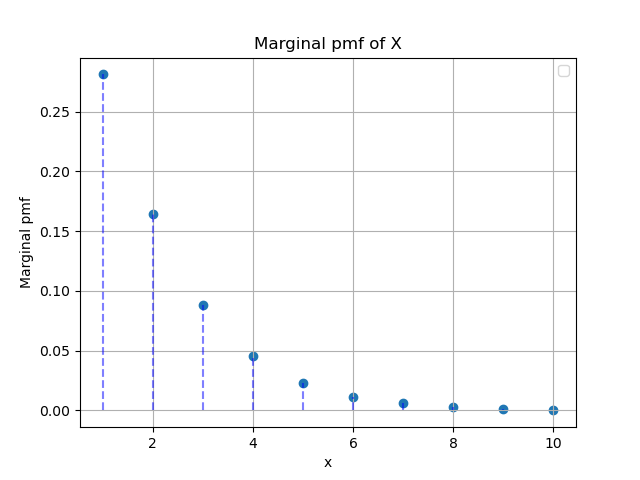
\includegraphics[width=\columnwidth]{/home/yogitha/47.2023/figs/pmfx.png}
\caption{Marginal pmf}
\label{fig:i_pmf}
\end{figure}
\end{enumerate}
Steps of simulation:
\begin{enumerate}
\item Define function p as $P\brak{x,y}=\frac{3}{2^{x+y+3}}$ in C and run a loop to sum the function p for all values of y except $x\neq y$, for each value of x.
\item Store values of marginal pmf for each value of x in a dat file 
\item Using plt.scatter function of python, plot the graph of Marginal pmf of X vs X.
The same can be used to plot marginal pmf of Y
\end{enumerate}

\item Let $(X,Y)$ have joint probability mass function
\begin{align}
p_{XY}\brak{x,y}&=
\begin{cases}
\frac{e^{-2}}{x!(y - x)!} & if x = 0,1,....,y; y = 0,1,2,....\\
0 & otherwise.\\
\end{cases}
\end{align}
Then which of the following statements is/are true?
\begin{enumerate}
\item ${E(X|Y = 4) = 2}$
\item The moment generating function of $Y$ is $e^{2(e^v - 1)}$ for all $v \in R$
\item ${E(X) = 2}$
\item The joint moment generating function of $(X,Y)$ is $e^{-2+(1 + e^u)e^v}$ for all $(u,v) \in {R^2}$
\end{enumerate}
\hfill(GATE ST 2023)\\
\iffalse
\let\negmedspace\undefined
\let\negthickspace\undefined
\documentclass[journal,12pt,twocolumn]{IEEEtran}
\usepackage{cite}
\usepackage{amsmath,amssymb,amsfonts,amsthm}
\usepackage{algorithmic}
\usepackage{graphicx}
\usepackage{textcomp}
\usepackage{xcolor}
\usepackage{txfonts}
\usepackage{listings}
\usepackage{enumitem}
\usepackage{mathtools}
\usepackage{gensymb}
\usepackage[breaklinks=true]{hyperref}
\usepackage{tkz-euclide} % loads  TikZ and tkz-base
\usepackage{listings}
\usepackage{gvv}
\usepackage{float}  % To use the [H] placement specifier

%
%\usepackage{setspace}
%\usepackage{gensymb}
%\doublespacing
%\singlespacing

%\usepackage{graphicx}
%\usepackage{amssymb}
%\usepackage{relsize}
%\usepackage[cmex10]{amsmath}
%\usepackage{amsthm}
%\interdisplaylinepenalty=2500
%\savesymbol{iint}
%\usepackage{txfonts}
%\restoresymbol{TXF}{iint}
%\usepackage{wasysym}
%\usepackage{amsthm}
%\usepackage{iithtlc}
%\usepackage{mathrsfs}
%\usepackage{txfonts}
%\usepackage{stfloats}
%\usepackage{bm}
%\usepackage{cite}
%\usepackage{cases}
%\usepackage{subfig}
%\usepackage{xtab}
%\usepackage{longtable}
%\usepackage{multirow}
%\usepackage{algorithm}
%\usepackage{algpseudocode}
%\usepackage{enumitem}
%\usepackage{mathtools}
%\usepackage{tikz}
%\usepackage{circuitikz}
%\usepackage{verbatim}
%\usepackage{tfrupee}
%\usepackage{stmaryrd}
%\usetkzobj{all}
%    \usepackage{color}                                            %%
%    \usepackage{array}                                            %%
%    \usepackage{longtable}                                        %%
%    \usepackage{calc}                                             %%
%    \usepackage{multirow}                                         %%
%    \usepackage{hhline}                                           %%
%    \usepackage{ifthen}                                           %%
  %optionally (for landscape tables embedded in another document): %%
%    \usepackage{lscape}     
%\usepackage{multicol}
%\usepackage{chngcntr}
%\usepackage{enumerate}

%\usepackage{wasysym}
%\documentclass[conference]{IEEEtran}
%\IEEEoverridecommandlockouts
% The preceding line is only needed to identify funding in the first footnote. If that is unneeded, please comment it out.

\newtheorem{theorem}{Theorem}[section]
\newtheorem{problem}{Problem}
\newtheorem{proposition}{Proposition}[section]
\newtheorem{lemma}{Lemma}[section]
\newtheorem{corollary}[theorem]{Corollary}
\newtheorem{example}{Example}[section]
\newtheorem{definition}[problem]{Definition}
%\newtheorem{thm}{Theorem}[section] 
%\newtheorem{defn}[thm]{Definition}
%\newtheorem{algorithm}{Algorithm}[section]
%\newtheorem{cor}{Corollary}
\newcommand{\BEQA}{\begin{eqnarray}}
\newcommand{\EEQA}{\end{eqnarray}}
%\newcommand{\define}{\stackrel{\triangle}{=}}
\theoremstyle{remark}
\newtheorem{rem}{Remark}

%\bibliographystyle{ieeetr}
\begin{document}
%

\bibliographystyle{IEEEtran}


\vspace{3cm}

\title{
%	\logo{
	47
%	}
}
\author{ EE22BTECH11059% <-this % stops a space
}	
%\title{
%	\logo{Matrix Analysis through Octave}{\begin{center}\includegraphics[scale=.24]{tlc}\end{center}}{}{HAMDSP}
%}


% paper title
% can use linebreaks \\ within to get better formatting as desired
%\title{Matrix Analysis through Octave}
%
%
% author names and IEEE memberships
% note positions of commas and nonbreaking spaces ( ~ ) LaTeX will not break
% a structure at a ~ so this keeps an author's name from being broken across
% two lines.
% use \thanks{} to gain access to the first footnote area
% a separate \thanks must be used for each paragraph as LaTeX2e's \thanks
% was not built to handle multiple paragraphs
%

%\author{<-this % stops a space
%\thanks{}}
%}
% note the % following the last \IEEEmembership and also \thanks - 
% these prevent an unwanted space from occurring between the last author name
% and the end of the author line. i.e., if you had this:
% 
% \author{....lastname \thanks{...} \thanks{...} }
%                     ^------------^------------^----Do not want these spaces!
%
% a space would be appended to the last name and could cause every name on that
% line to be shifted left slightly. This is one of those "LaTeX things". For
% instance, "\textbf{A} \textbf{B}" will typeset as "A B" not "AB". To get
% "AB" then you have to do: "\textbf{A}\textbf{B}"
% \thanks is no different in this regard, so shield the last } of each \thanks
% that ends a line with a % and do not let a space in before the next \thanks.
% Spaces after \IEEEmembership other than the last one are OK (and needed) as
% you are supposed to have spaces between the names. For what it is worth,
% this is a minor point as most people would not even notice if the said evil
% space somehow managed to creep in.



% The paper headers
%\markboth{Journal of \LaTeX\ Class Files,~Vol.~6, No.~1, January~2007}%
%{Shell \MakeLowercase{\textit{et al.}}: Bare Demo of IEEEtran.cls for Journals}
% The only time the second header will appear is for the odd numbered pages
% after the title page when using the twoside option.
% 
% *** Note that you probably will NOT want to include the author's ***
% *** name in the headers of peer review papers.                   ***
% You can use \ifCLASSOPTIONpeerreview for conditional compilation here if
% you desire.




% If you want to put a publisher's ID mark on the page you can do it like
% this:
%\IEEEpubid{0000--0000/00\$00.00~\copyright~2007 IEEE}
% Remember, if you use this you must call \IEEEpubidadjcol in the second
% column for its text to clear the IEEEpubid mark.



% make the title area
\maketitle

\newpage

%\tableofcontents

\bigskip

\renewcommand{\thefigure}{\theenumi}
\renewcommand{\thetable}{\theenumi}
%\renewcommand{\theequation}{\theenumi}

%\begin{abstract}
%%\boldmath
%In this letter, an algorithm for evaluating the exact analytical bit error rate  (BER)  for the piecewise linear (PL) combiner for  multiple relays is presented. Previous results were available only for upto three relays. The algorithm is unique in the sense that  the actual mathematical expressions, that are prohibitively large, need not be explicitly obtained. The diversity gain due to multiple relays is shown through plots of the analytical BER, well supported by simulations. 
%
%\end{abstract}
% IEEEtran.cls defaults to using nonbold math in the Abstract.
% This preserves the distinction between vectors and scalars. However,
% if the journal you are submitting to favors bold math in the abstract,
% then you can use LaTeX's standard command \boldmath at the very start
% of the abstract to achieve this. Many IEEE journals frown on math
% in the abstract anyway.

% Note that keywords are not normally used for peerreview papers.
%\begin{IEEEkeywords}
%Cooperative diversity, decode and forward, piecewise linear
%\end{IEEEkeywords}



% For peer review papers, you can put extra information on the cover
% page as needed:
% \ifCLASSOPTIONpeerreview
% \begin{center} \bfseries EDICS Category: 3-BBND \end{center}
% \fi
%
% For peerreview papers, this IEEEtran command inserts a page break and
% creates the second title. It will be ignored for other modes.
%\IEEEpeerreviewmaketitle

%\documentclass{article}
%\usepackage{amsmath}
%\section*{ASSIGNMENT 1}
Let \brak{X,Y} have joint probability mass function 
\begin{align}
p\brak{x,y}=  
	\begin{cases}
        \frac{c}{2^{x+y+2}} & if x=0,1,2,... \, y=0,1,2,...; x\neq y \\
        0 & otherwise
        \end{cases} 
\end{align} 
Then which of the following is true?\\
\hfill (GATE ST 2023) \\
\begin{enumerate}
\item $c = \frac{1}{2}$
\item $c = \frac{1}{4}$
\item $c > 1$
\item $X$ and $Y$ are independent
\end{enumerate}
\fi
\solution
For p\brak{x,y} to be joint probability mass function
\begin{align}
\sum\limits^{\infty}_{y=-\infty}\sum\limits^{\infty}_{x=-\infty}p(x,y)&=1 \, \vert x \neq y\\
\sum\limits^{\infty}_{y=0}\sum\limits^{\infty}_{x=0}\frac{c}{2^{x+y+2}}- \sum\limits_{x=y} \frac{c}{2^{x+y+2}}&=1\\
\sum\limits^{\infty}_{y=0}\frac{c}{2^{y+2}} \sum\limits^{\infty}_{x=0} 2^{-x}- \frac{c}{4}\sum\limits^{\infty}_{x=0}\frac{1}{4^x}&=1\\
\sum\limits^{\infty}_{y=0}\frac{2c}{2^{y+2}}- \frac{c}{3}&=1\\
\frac{2c}{4}\sum\limits^{\infty}_{y=0}2^{-y}-\frac{c}{3}&=1\\
c-\frac{c}{3}&=1\\
c&=\frac{3}{2}
\end{align}
\begin{enumerate}
\item Marginal probability mass function of X
\begin{align}
p_X\brak{x}&=\sum\limits^{\infty}_{y=0}p\brak{x,y} \vert x \neq y\\
&=\sum\limits^{\infty}_{y=0}\frac{3}{2^{x+y+3}}- p_{XY}\brak{x,x}\\
&=\frac{3}{2^{x+3}}\sum\limits^{\infty}_{y=0}2^{-y}-\frac{3}{2^{2x+3}}\\
&=\frac{3}{2^{x+2}}-\frac{3}{2^{2x+3}}
\end{align}
\item Marginal cdf of X
\begin{align}
F_X\brak{x}&=\sum\limits^{x}_{i=0} p_X\brak{X \leq x}\\
&=\sum\limits^{x}_{i=0}\brak{\frac{3}{2^{x+2}}-\frac{3}{2^{2x+3}}}\\
&=1+\frac{1}{2^{x+2}}-\frac{3}{2^{2x+3}}
\end{align}
\item Marginal probability mass function of Y
\begin{align}
p_Y\brak{y}&=\sum\limits^{\infty}_{x=0}p\brak{x,y} \vert x \neq y\\
&=\sum\limits^{\infty}_{x=0}\frac{3}{2^{x+y+3}}- p_{XY}\brak{y,y}\\
&=\frac{3}{2^{y+3}}\sum\limits^{\infty}_{x=0}2^{-x}-\frac{3}{2^{2y+3}}\\
&=\frac{3}{2^{y+2}}-\frac{3}{2^{2y+3}}\\
\end{align}
\item Marginal cdf of Y
\begin{align}
F_Y\brak{y}&=\sum\limits^{y}_{i=0} p_Y\brak{Y \leq y}\\
&=\sum\limits^{y}_{i=0}\brak{\frac{3}{2^{y+2}}-\frac{3}{2^{2y+3}}}\\
&=1+\frac{1}{2^{y+2}}-\frac{3}{2^{2y+3}}
\end{align}
\item For X and Y to be independent,
\begin{align}
p\brak{x,y}&=p_X\brak{x} p_Y\brak{y}\\
p_X\brak{x} p_Y\brak{y}&=\brak{\frac{3}{2^{x+2}}-\frac{3}{2^{2x+3}}}\brak{\frac{3}{2^{y+2}}-\frac{3}{2^{2y+3}}}\\
p\brak{x,y} &\neq p_X\brak{x} p_Y\brak{y}
\end{align}
\end{enumerate}
Option \brak{4} is incorrect.\\
$\therefore$ Only option \brak{3} is correct. \\
Simulations:
\begin{enumerate}
\item Marginal pmf of X
\begin{figure}[H]
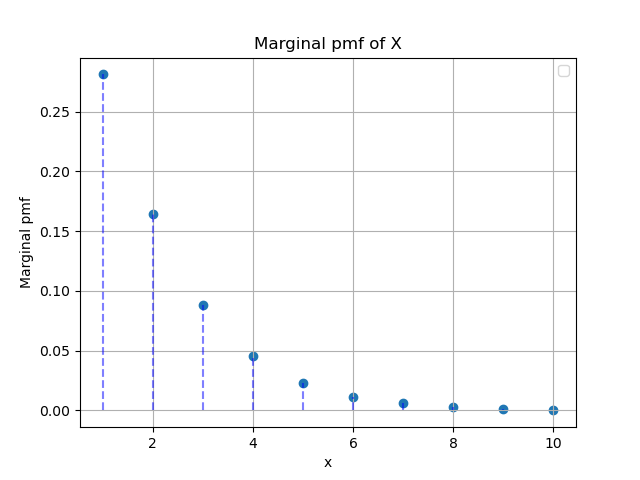
\includegraphics[width=\columnwidth]{/home/yogitha/47.2023/figs/pmfx.png}
\caption{Marginal pmf}
\label{fig:i_pmf}
\end{figure}
\end{enumerate}
Steps of simulation:
\begin{enumerate}
\item Define function p as $P\brak{x,y}=\frac{3}{2^{x+y+3}}$ in C and run a loop to sum the function p for all values of y except $x\neq y$, for each value of x.
\item Store values of marginal pmf for each value of x in a dat file 
\item Using plt.scatter function of python, plot the graph of Marginal pmf of X vs X.
The same can be used to plot marginal pmf of Y
\end{enumerate}

\item Let \brak{X,Y} have joint probability mass function 
\begin{align}
p\brak{x,y}=  
	\begin{cases}
        \frac{c}{2^{x+y+2}} & if x=0,1,2,... \, y=0,1,2,...; x\neq y \\
        0 & otherwise
        \end{cases} 
\end{align} 
Then which of the following is true?
\begin{enumerate}
\item $c = \frac{1}{2}$
\item $c = \frac{1}{4}$
\item $c > 1$
\item $X$ and $Y$ are independent
\end{enumerate}
\hfill(GATE ST 2023)\\
\iffalse
\let\negmedspace\undefined
\let\negthickspace\undefined
\documentclass[journal,12pt,twocolumn]{IEEEtran}
\usepackage{cite}
\usepackage{amsmath,amssymb,amsfonts,amsthm}
\usepackage{algorithmic}
\usepackage{graphicx}
\usepackage{textcomp}
\usepackage{xcolor}
\usepackage{txfonts}
\usepackage{listings}
\usepackage{enumitem}
\usepackage{mathtools}
\usepackage{gensymb}
\usepackage[breaklinks=true]{hyperref}
\usepackage{tkz-euclide} % loads  TikZ and tkz-base
\usepackage{listings}
\usepackage{gvv}
\usepackage{float}  % To use the [H] placement specifier

%
%\usepackage{setspace}
%\usepackage{gensymb}
%\doublespacing
%\singlespacing

%\usepackage{graphicx}
%\usepackage{amssymb}
%\usepackage{relsize}
%\usepackage[cmex10]{amsmath}
%\usepackage{amsthm}
%\interdisplaylinepenalty=2500
%\savesymbol{iint}
%\usepackage{txfonts}
%\restoresymbol{TXF}{iint}
%\usepackage{wasysym}
%\usepackage{amsthm}
%\usepackage{iithtlc}
%\usepackage{mathrsfs}
%\usepackage{txfonts}
%\usepackage{stfloats}
%\usepackage{bm}
%\usepackage{cite}
%\usepackage{cases}
%\usepackage{subfig}
%\usepackage{xtab}
%\usepackage{longtable}
%\usepackage{multirow}
%\usepackage{algorithm}
%\usepackage{algpseudocode}
%\usepackage{enumitem}
%\usepackage{mathtools}
%\usepackage{tikz}
%\usepackage{circuitikz}
%\usepackage{verbatim}
%\usepackage{tfrupee}
%\usepackage{stmaryrd}
%\usetkzobj{all}
%    \usepackage{color}                                            %%
%    \usepackage{array}                                            %%
%    \usepackage{longtable}                                        %%
%    \usepackage{calc}                                             %%
%    \usepackage{multirow}                                         %%
%    \usepackage{hhline}                                           %%
%    \usepackage{ifthen}                                           %%
  %optionally (for landscape tables embedded in another document): %%
%    \usepackage{lscape}     
%\usepackage{multicol}
%\usepackage{chngcntr}
%\usepackage{enumerate}

%\usepackage{wasysym}
%\documentclass[conference]{IEEEtran}
%\IEEEoverridecommandlockouts
% The preceding line is only needed to identify funding in the first footnote. If that is unneeded, please comment it out.

\newtheorem{theorem}{Theorem}[section]
\newtheorem{problem}{Problem}
\newtheorem{proposition}{Proposition}[section]
\newtheorem{lemma}{Lemma}[section]
\newtheorem{corollary}[theorem]{Corollary}
\newtheorem{example}{Example}[section]
\newtheorem{definition}[problem]{Definition}
%\newtheorem{thm}{Theorem}[section] 
%\newtheorem{defn}[thm]{Definition}
%\newtheorem{algorithm}{Algorithm}[section]
%\newtheorem{cor}{Corollary}
\newcommand{\BEQA}{\begin{eqnarray}}
\newcommand{\EEQA}{\end{eqnarray}}
%\newcommand{\define}{\stackrel{\triangle}{=}}
\theoremstyle{remark}
\newtheorem{rem}{Remark}

%\bibliographystyle{ieeetr}
\begin{document}
%

\bibliographystyle{IEEEtran}


\vspace{3cm}

\title{
%	\logo{
	47
%	}
}
\author{ EE22BTECH11059% <-this % stops a space
}	
%\title{
%	\logo{Matrix Analysis through Octave}{\begin{center}\includegraphics[scale=.24]{tlc}\end{center}}{}{HAMDSP}
%}


% paper title
% can use linebreaks \\ within to get better formatting as desired
%\title{Matrix Analysis through Octave}
%
%
% author names and IEEE memberships
% note positions of commas and nonbreaking spaces ( ~ ) LaTeX will not break
% a structure at a ~ so this keeps an author's name from being broken across
% two lines.
% use \thanks{} to gain access to the first footnote area
% a separate \thanks must be used for each paragraph as LaTeX2e's \thanks
% was not built to handle multiple paragraphs
%

%\author{<-this % stops a space
%\thanks{}}
%}
% note the % following the last \IEEEmembership and also \thanks - 
% these prevent an unwanted space from occurring between the last author name
% and the end of the author line. i.e., if you had this:
% 
% \author{....lastname \thanks{...} \thanks{...} }
%                     ^------------^------------^----Do not want these spaces!
%
% a space would be appended to the last name and could cause every name on that
% line to be shifted left slightly. This is one of those "LaTeX things". For
% instance, "\textbf{A} \textbf{B}" will typeset as "A B" not "AB". To get
% "AB" then you have to do: "\textbf{A}\textbf{B}"
% \thanks is no different in this regard, so shield the last } of each \thanks
% that ends a line with a % and do not let a space in before the next \thanks.
% Spaces after \IEEEmembership other than the last one are OK (and needed) as
% you are supposed to have spaces between the names. For what it is worth,
% this is a minor point as most people would not even notice if the said evil
% space somehow managed to creep in.



% The paper headers
%\markboth{Journal of \LaTeX\ Class Files,~Vol.~6, No.~1, January~2007}%
%{Shell \MakeLowercase{\textit{et al.}}: Bare Demo of IEEEtran.cls for Journals}
% The only time the second header will appear is for the odd numbered pages
% after the title page when using the twoside option.
% 
% *** Note that you probably will NOT want to include the author's ***
% *** name in the headers of peer review papers.                   ***
% You can use \ifCLASSOPTIONpeerreview for conditional compilation here if
% you desire.




% If you want to put a publisher's ID mark on the page you can do it like
% this:
%\IEEEpubid{0000--0000/00\$00.00~\copyright~2007 IEEE}
% Remember, if you use this you must call \IEEEpubidadjcol in the second
% column for its text to clear the IEEEpubid mark.



% make the title area
\maketitle

\newpage

%\tableofcontents

\bigskip

\renewcommand{\thefigure}{\theenumi}
\renewcommand{\thetable}{\theenumi}
%\renewcommand{\theequation}{\theenumi}

%\begin{abstract}
%%\boldmath
%In this letter, an algorithm for evaluating the exact analytical bit error rate  (BER)  for the piecewise linear (PL) combiner for  multiple relays is presented. Previous results were available only for upto three relays. The algorithm is unique in the sense that  the actual mathematical expressions, that are prohibitively large, need not be explicitly obtained. The diversity gain due to multiple relays is shown through plots of the analytical BER, well supported by simulations. 
%
%\end{abstract}
% IEEEtran.cls defaults to using nonbold math in the Abstract.
% This preserves the distinction between vectors and scalars. However,
% if the journal you are submitting to favors bold math in the abstract,
% then you can use LaTeX's standard command \boldmath at the very start
% of the abstract to achieve this. Many IEEE journals frown on math
% in the abstract anyway.

% Note that keywords are not normally used for peerreview papers.
%\begin{IEEEkeywords}
%Cooperative diversity, decode and forward, piecewise linear
%\end{IEEEkeywords}



% For peer review papers, you can put extra information on the cover
% page as needed:
% \ifCLASSOPTIONpeerreview
% \begin{center} \bfseries EDICS Category: 3-BBND \end{center}
% \fi
%
% For peerreview papers, this IEEEtran command inserts a page break and
% creates the second title. It will be ignored for other modes.
%\IEEEpeerreviewmaketitle

%\documentclass{article}
%\usepackage{amsmath}
%\section*{ASSIGNMENT 1}
Let \brak{X,Y} have joint probability mass function 
\begin{align}
p\brak{x,y}=  
	\begin{cases}
        \frac{c}{2^{x+y+2}} & if x=0,1,2,... \, y=0,1,2,...; x\neq y \\
        0 & otherwise
        \end{cases} 
\end{align} 
Then which of the following is true?\\
\hfill (GATE ST 2023) \\
\begin{enumerate}
\item $c = \frac{1}{2}$
\item $c = \frac{1}{4}$
\item $c > 1$
\item $X$ and $Y$ are independent
\end{enumerate}
\fi
\solution
For p\brak{x,y} to be joint probability mass function
\begin{align}
\sum\limits^{\infty}_{y=-\infty}\sum\limits^{\infty}_{x=-\infty}p(x,y)&=1 \, \vert x \neq y\\
\sum\limits^{\infty}_{y=0}\sum\limits^{\infty}_{x=0}\frac{c}{2^{x+y+2}}- \sum\limits_{x=y} \frac{c}{2^{x+y+2}}&=1\\
\sum\limits^{\infty}_{y=0}\frac{c}{2^{y+2}} \sum\limits^{\infty}_{x=0} 2^{-x}- \frac{c}{4}\sum\limits^{\infty}_{x=0}\frac{1}{4^x}&=1\\
\sum\limits^{\infty}_{y=0}\frac{2c}{2^{y+2}}- \frac{c}{3}&=1\\
\frac{2c}{4}\sum\limits^{\infty}_{y=0}2^{-y}-\frac{c}{3}&=1\\
c-\frac{c}{3}&=1\\
c&=\frac{3}{2}
\end{align}
\begin{enumerate}
\item Marginal probability mass function of X
\begin{align}
p_X\brak{x}&=\sum\limits^{\infty}_{y=0}p\brak{x,y} \vert x \neq y\\
&=\sum\limits^{\infty}_{y=0}\frac{3}{2^{x+y+3}}- p_{XY}\brak{x,x}\\
&=\frac{3}{2^{x+3}}\sum\limits^{\infty}_{y=0}2^{-y}-\frac{3}{2^{2x+3}}\\
&=\frac{3}{2^{x+2}}-\frac{3}{2^{2x+3}}
\end{align}
\item Marginal cdf of X
\begin{align}
F_X\brak{x}&=\sum\limits^{x}_{i=0} p_X\brak{X \leq x}\\
&=\sum\limits^{x}_{i=0}\brak{\frac{3}{2^{x+2}}-\frac{3}{2^{2x+3}}}\\
&=1+\frac{1}{2^{x+2}}-\frac{3}{2^{2x+3}}
\end{align}
\item Marginal probability mass function of Y
\begin{align}
p_Y\brak{y}&=\sum\limits^{\infty}_{x=0}p\brak{x,y} \vert x \neq y\\
&=\sum\limits^{\infty}_{x=0}\frac{3}{2^{x+y+3}}- p_{XY}\brak{y,y}\\
&=\frac{3}{2^{y+3}}\sum\limits^{\infty}_{x=0}2^{-x}-\frac{3}{2^{2y+3}}\\
&=\frac{3}{2^{y+2}}-\frac{3}{2^{2y+3}}\\
\end{align}
\item Marginal cdf of Y
\begin{align}
F_Y\brak{y}&=\sum\limits^{y}_{i=0} p_Y\brak{Y \leq y}\\
&=\sum\limits^{y}_{i=0}\brak{\frac{3}{2^{y+2}}-\frac{3}{2^{2y+3}}}\\
&=1+\frac{1}{2^{y+2}}-\frac{3}{2^{2y+3}}
\end{align}
\item For X and Y to be independent,
\begin{align}
p\brak{x,y}&=p_X\brak{x} p_Y\brak{y}\\
p_X\brak{x} p_Y\brak{y}&=\brak{\frac{3}{2^{x+2}}-\frac{3}{2^{2x+3}}}\brak{\frac{3}{2^{y+2}}-\frac{3}{2^{2y+3}}}\\
p\brak{x,y} &\neq p_X\brak{x} p_Y\brak{y}
\end{align}
\end{enumerate}
Option \brak{4} is incorrect.\\
$\therefore$ Only option \brak{3} is correct. \\
Simulations:
\begin{enumerate}
\item Marginal pmf of X
\begin{figure}[H]
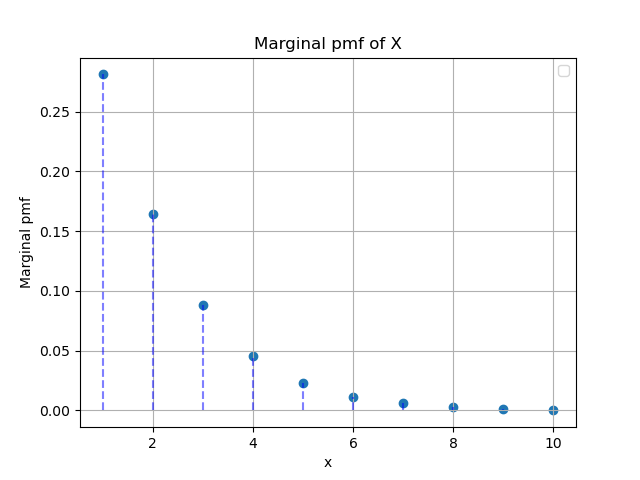
\includegraphics[width=\columnwidth]{/home/yogitha/47.2023/figs/pmfx.png}
\caption{Marginal pmf}
\label{fig:i_pmf}
\end{figure}
\end{enumerate}
Steps of simulation:
\begin{enumerate}
\item Define function p as $P\brak{x,y}=\frac{3}{2^{x+y+3}}$ in C and run a loop to sum the function p for all values of y except $x\neq y$, for each value of x.
\item Store values of marginal pmf for each value of x in a dat file 
\item Using plt.scatter function of python, plot the graph of Marginal pmf of X vs X.
The same can be used to plot marginal pmf of Y
\end{enumerate}

\end{enumerate}
